% !TeX program = xelatex
% !TeX TXS-program:compile = txs:///xelatex/[--shell-escape]
%%%%%%%%%%%%%%%%%%%%%%%%%%%%%%%%%%%%%%%%%%%%%%%%%%%%%%%%%%%%%%%%%%%%%%%%
% Plantilla TFG/TFM
% Escuela Politécnica Superior de la Universidad de Alicante
% Realizado por: Jose Manuel Requena Plens
% Contacto: info@jmrplens.com / Telegram:@jmrplens
%%%%%%%%%%%%%%%%%%%%%%%%%%%%%%%%%%%%%%%%%%%%%%%%%%%%%%%%%%%%%%%%%%%%%%%%

% Elige si deseas optimizar la ejecución del proyecto almacenando las figuras generadas con TikZ y PGF en una carpeta (archivos/figuras-procesadas).
% 1 - Si, 2 - No
\def\OptimizaTikZ{1}

% Archivo .TEX que incluye todas las configuraciones del documento y los paquetes. Añade todo aquello que necesites utilizar en el documento en este archivo.
% En él se encuentra la configuración de los márgenes, establecidos según las directrices de estilo de la EPS.
%%%%%%%%%%%%%%%%%%%%%%%%%%%%%%%%%%%%%%%%%%%%%%%%%%%%%%%%%%%%%%%%%%%%%%%%
% Plantilla TFG/TFM
% Escuela Politécnica Superior de la Universidad de Alicante
% Realizado por: Jose Manuel Requena Plens
% Contacto: info@jmrplens.com / Telegram:@jmrplens
%%%%%%%%%%%%%%%%%%%%%%%%%%%%%%%%%%%%%%%%%%%%%%%%%%%%%%%%%%%%%%%%%%%%%%%%

%%%%%%%%%%%%%%%%%%%%%%%%
% FORMATO DEL DOCUMENTO
%%%%%%%%%%%%%%%%%%%%%%%%
% scrbook es la clase de documento
% Si se desea que no haya página en blanco entre capítulos añadir "openany" en los parámetros de la clase. Sino siempre los capítulos empezarán en página impar.
\documentclass[a4paper,11pt,titlepage]{scrbook}
\KOMAoption{toc}{bib,chapterentryfill} % Opciones del índice
\usepackage{scrhack} % Previene algunos errores
% Paquete de formato para scrbook. Con marcas, linea-separador superior e inferior
\usepackage[automark,headsepline,footsepline]{scrlayer-scrpage}
\clearpairofpagestyles		% Borra los estilos por defecto
%%
% Formato y contenido de la información de cabecera y pie de página
%%
% Información de capítulo en cabecera e interno
\ihead{{\color{gray30}\scshape\small\headmark}}	
% Número de página en cabecera y externo
\ohead{\normalfont\pagemark} 
% Número de página en pie de página y externo. Sólo en páginas sin cabecera
\ofoot[\normalfont\pagemark]{}
%% 		
% Edición del contenido de las distintas partes de la cabecera
%%
\renewcommand{\chaptermark}[1]{\markboth{#1}{}} % Capítulo (Solo texto)
\renewcommand{\sectionmark}[1]{\markright{\thesection. #1}} % Sección (Número y texto)
\setkomafont{pagenumber}{} % Número de página (Sin nada añadido)

% Añade al índice y numera hasta la profundidad 4.
% 1:section,2:subsection,3:subsubsection,4:paragraph
\setcounter{tocdepth}{4}
\setcounter{secnumdepth}{4}
% Muestra una regla para comprobar el formato de las páginas
%\usepackage[type=upperleft,showframe,marklength=8mm]{fgruler}
% MÁRGENES DE LAS PÁGINAS
\usepackage[
  inner	=	3.0cm, % Margen interior
  outer	=	2.5cm, % Margen exterior
  top	=	2.5cm, % Margen superior
  bottom=	2.5cm, % Margen inferior
  includeheadfoot, % Incluye cabecera y pie de página en los márgenes
]{geometry}
% Valor de interlineado
\renewcommand{\baselinestretch}{1.0} % 1 línea de interlineado
% Para poder generar páginas horizontales
\usepackage{lscape}
% Ancho de la zona para comentarios en el margen. (modificado para todonotes)
\setlength{\marginparwidth}{1.9cm}

%%%%%%%%%%%%%%%%%%%%%%%%
% BIBLIOGRAFÍA
%%%%%%%%%%%%%%%%%%%%%%%%
\usepackage{apacite} % NORMA APA
\usepackage{natbib}
\usepackage{breakcites}

%%%%%%%%%%%%%%%%%%%%%%%%
% DOCUMENTO EN ESPAÑOL
%%%%%%%%%%%%%%%%%%%%%%%%
\usepackage[base]{babel}
\usepackage{polyglossia}
\setdefaultlanguage{spanish}

\addto\captionsspanish{%
	\renewcommand{\listtablename}{Índice de tablas} 
	\renewcommand{\tablename}{Tabla}
	\renewcommand{\lstlistingname}{Código}
	\renewcommand{\lstlistlistingname}{Índice de \lstlistingname s}
	\renewcommand{\glossaryname}{Glosario}
	\renewcommand{\acronymname}{Acrónimos}
	\renewcommand{\bibname}{Bibliografía}%
}

%%%%%%%%%%%%%%%%%%%%%%%% 
% COLORES
%%%%%%%%%%%%%%%%%%%%%%%% 
% Biblioteca de colores
\usepackage{color}
\usepackage[dvipsnames]{xcolor}
% Otros colores definidos por el usuario
\definecolor{gray97}{gray}{.97}
\definecolor{gray75}{gray}{.75}
\definecolor{gray45}{gray}{.45}
\definecolor{gray30}{gray}{.30}
\definecolor{negro}{RGB}{0,0,0}
\definecolor{blanco}{RGB}{255,255,255}
\definecolor{dkgreen}{rgb}{0,.6,0}
\definecolor{dkblue}{rgb}{0,0,.6}
\definecolor{dkyellow}{cmyk}{0,0,.8,.3}
\definecolor{gray}{rgb}{0.5,0.5,0.5}
\definecolor{mauve}{rgb}{0.58,0,0.82}
\definecolor{deepblue}{rgb}{0,0,0.5}
\definecolor{deepred}{rgb}{0.6,0,0}
\definecolor{deepgreen}{rgb}{0,0.5,0}
\definecolor{MyDarkGreen}{rgb}{0.0,0.4,0.0}
\definecolor{bluekeywords}{rgb}{0.13,0.13,1}
\definecolor{greencomments}{rgb}{0,0.5,0}
\definecolor{redstrings}{rgb}{0.9,0,0}

%%%%%%%%%%%%%%%%%%%%%%%%
% TABLAS
%%%%%%%%%%%%%%%%%%%%%%%%
% Paquetes para tablas
\usepackage{longtable,booktabs,array,multirow,multicol,tabularx,ragged2e,array}
% Nuevos tipos de columna para tabla, se pueden utilizar como por ejemplo C{3cm} en la definición de columnas de la función tabular
\newcolumntype{L}[1]{>{\raggedright\let\newline\\\arraybackslash\hspace{0pt}}m{#1}}
\newcolumntype{C}[1]{>{\centering\let\newline\\\arraybackslash\hspace{0pt}}m{#1}}
\newcolumntype{R}[1]{>{\raggedleft\let\newline\\\arraybackslash\hspace{0pt}}m{#1}}

%%%%%%%%%%%%%%%%%%%%%%%% 
% GRAFICAS y DIAGRAMAS 
%%%%%%%%%%%%%%%%%%%%%%%% 
% Paquete para todo tipo de gráficas, diagramas, modificación de imágenes, etc
\usepackage{tikz,tikzpagenodes}
\usetikzlibrary{tikzmark,calc,shapes.geometric,arrows,backgrounds,shadings,shapes.arrows,shapes.symbols,shadows,positioning,fit,automata,patterns,intersections}
\usepackage{pgfplots}
\pgfplotsset{colormap/jet}
\pgfplotsset{compat=newest} % Compatibilidad
\usepgfplotslibrary{patchplots,groupplots,fillbetween,polar}
\usepackage{pgfplotstable}
% Guardar las figuras realizadas con Tikz y Pgf en una carpeta externa
% para agilizar el procesado y tenerlas para utilizarlas en otros
% documentos
\if\OptimizaTikZ 1
\usepgfplotslibrary{external}
\tikzexternalize[prefix=archivos/figuras-procesadas/] % Ruta
\tikzset{%
    external/system call ={xelatex -enable-write18 -halt-on-error -interaction=batchmode -jobname "\image" "\texsource"},
}
\fi

% Estilos para elementos graficos
% Cajas y cajas de texto
\tikzstyle{Caja1} = [green,very thick,rounded corners,fill=white, fill opacity=0.5]
\tikzstyle{Texto1} = [fill=white,thick,shape=circle,draw=black,inner sep=2pt,font=\sffamily,text=black]
\tikzstyle{Texto2} = [fill=white,thick,shape=rectangle,draw=black,inner sep=2pt,font=\sffamily,text=black]
\tikzstyle{Texto3} = [fill=white,thick,shape=circle,draw=black,inner sep=2pt,font=\sffamily,text=black]
% Cuadros de diagrama
\tikzstyle{rectvioleta} = [rectangle, rounded corners, text centered, draw=black, fill=blue!10]
\tikzstyle{rectnaranja} = [rectangle, minimum width=2cm, minimum height=1cm, text centered, draw=black, fill=orange!10]
\tikzstyle{romborosa} = [diamond, aspect=3, minimum width=3cm, minimum height=1cm, text centered, draw=black, fill=red!10]
\tikzstyle{rectverde} = [rectangle, minimum width=2cm, minimum height=1cm, text centered, draw=black, fill=green!10]
\tikzstyle{rectamarillo} = [rectangle, rounded corners, minimum width=2cm, minimum height=1cm, text centered, draw=black, fill=yellow!10]
% Flechas
\tikzstyle{arrow} = [thick,->,>=stealth]

%%%%%%%%%%%%%%%%%%%%%%%% 
% FIGURAS, TABLAS, ETC 
%%%%%%%%%%%%%%%%%%%%%%%% 
\usepackage{subcaption} % Para poder realizar subfiguras
\usepackage{caption} % Para aumentar las opciones de diseño
% Nombres de figuras, tablas, etc, en negrita la numeración, todo con letra small
\captionsetup{labelfont={bf,small},textfont=small}
% Paquete para modificar los espacios arriba y abajo de una figura o tabla
\usepackage{setspace}
% Define el espacio tanto arriba como abajo de las figuras, tablas
\setlength{\intextsep}{5mm}
% Para ajustar tamaños de texto de toda una tabla o grafica
% Uso: {\scalefont{0.8} \begin{...} \end{...} }
\usepackage{scalefnt}
% Redefine las tablas y figuras para eliminar el '.' entre la numeración y el texto
\renewcommand*{\figureformat}{\figurename~\thefigure}
\renewcommand*{\tableformat}{\tablename~\thetable}

%%%%%%%%%%%%%%%%%%%%%%%% 
% TEXTO
%%%%%%%%%%%%%%%%%%%%%%%%
% Paquete para poder modificar las fuente de texto
\usepackage{xltxtra}
% Cualquier tamaño de texto. Uso: {\fontsize{100pt}{120pt}\selectfont tutexto}
\usepackage{anyfontsize}
% Para modificar parametros del texto.
\usepackage{setspace}
% Paquete para posicionar bloques de texto
\usepackage{textpos}
% Paquete para realizar cajas de texto. 
% Uso: \begin{mdframed}[linecolor=red!100!black] tutexto \end{mdframed}
\usepackage{framed,mdframed}
% Para subrayar. Uso: \hlc[tucolor]{tutexto}
\newcommand{\hlc}[2][yellow]{ {\sethlcolor{#1} \hl{#2}} }

%%%%%%%%%%%%%%%%%%%%%%%% 
% OTROS
%%%%%%%%%%%%%%%%%%%%%%%%
% Para hacer una pagina horizontal. Uso: \begin{landscape} xxxx \end{lanscape}
\usepackage{lscape} 
% Para incluir paginas PDF. Uso:
% \includepdf[pages={1}]{tuarchivo.pdf}
\usepackage{pdfpages}
% Para introducir url's con formato. Uso: \url{http://www.google.es}
\usepackage{url}
% Amplia muchas funciones graficas de latex
\usepackage{graphicx}
% Paquete que añade el hipervinculo en referencias dentro del documento, indice, etc
% Se define sin bordes alrededor. Uso: \ref{tulabel}
\usepackage[pdfborder={000}]{hyperref}
\usepackage{float}
\usepackage{placeins}
\usepackage{afterpage}
\usepackage{verbatim}
% Paquete para condicionales avanzados
\usepackage{xstring,xifthen}
% Paquete para realizar calculos en el código
\usepackage{calc}
% Para rotar tablas o figuras o su contenido
\usepackage{rotating} 
% Para incluir comentarios en el texto. El parámetro 'disable' oculta todas las notas.
% USO: \todo{tutexto}
\usepackage[textsize=tiny,spanish,shadow,textwidth=2cm]{todonotes}
%\reversemarginpar % Descomentar si se quiere todos los comentarios en el mismo lado
% Desactiva la exportación de los ToDo y Missingfigures como figuras
\if\OptimizaTikZ 1
\makeatletter
\renewcommand{\todo}[2][]{\tikzexternaldisable\@todo[#1]{#2}\tikzexternalenable}
\makeatother
\usepackage{letltxmacro}
\LetLtxMacro{\oldmissingfigure}{\missingfigure}
\makeatletter
\renewcommand{\missingfigure}[2][]{\tikzexternaldisable\oldmissingfigure[{#1}]{#2}\tikzexternalenable}
\makeatother
\fi

%%%%%%%%%%%%%%%%%%%%%%%% 
% GLOSARIOS
%%%%%%%%%%%%%%%%%%%%%%%%
\usepackage[acronym,nonumberlist,toc]{glossaries}
\usepackage{glossary-superragged}
\newglossarystyle{modsuper}{%
  \setglossarystyle{super}%
  \renewcommand{\glsgroupskip}{}
}
\renewcommand{\glsnamefont}[1]{\textbf{#1}}


%%%%%%%%%%%%%%%%%%%%%%%% 
% COMANDOS AÑADIDOS
%%%%%%%%%%%%%%%%%%%%%%%%
% Para mostrar la fecha actual (mes año) con \Hoy
\newcommand{\MES}{%
  \ifcase\month% 0
    \or Enero% 1
    \or Febrero% 2
    \or Marzo% 3
    \or Abril% 4
    \or Mayo% 5
    \or Junio% 6
    \or Julio% 7
    \or Agosto% 8
    \or Septiembre% 9
    \or Octubre% 10
    \or Noviembre% 11
    \or Diciembre% 12
  \fi}
\newcommand{\ANYO}{\number\year}
\newcommand{\Hoy}{\MES\ \ANYO}

%%%%%%%%%%%%%%%%%%%%%%%% 
% MATEMÁTICAS
%%%%%%%%%%%%%%%%%%%%%%%%
\usepackage{mathtools,amsthm,amsfonts,amssymb,bm,mathrsfs,nicefrac,upgreek,bigints} 
% Comando para añadir información de variables a las ecuaciones
% Uso: \begin{condiciones}[donde:] ....... \end{condiciones}
\newenvironment{condiciones}[1][2]
  {%
   #1\tabularx{\textwidth-\widthof{#1}}[t]{
     >{$}l<{$} @{}>{${}}c<{{}$}@{} >{\raggedright\arraybackslash}X
   }%
  }
  {\endtabularx\\[\belowdisplayskip]}

%%%%%
% PARÁMETROS DE FORMATO DE CODIGOS
%%%%%
% Puedes editar los formatos para ajustarlos a tu gusto
%%%%%%%%%%%%%%%%%%%%%%%%%%%%%%%%%%%%%%%%%%%%%%%%%%%%%%%%%%%%%%%%%%%%%%%%
% Plantilla TFG/TFM
% Escuela Politécnica Superior de la Universidad de Alicante
% Realizado por: Jose Manuel Requena Plens
% Contacto: info@jmrplens.com / Telegram:@jmrplens
%%%%%%%%%%%%%%%%%%%%%%%%%%%%%%%%%%%%%%%%%%%%%%%%%%%%%%%%%%%%%%%%%%%%%%%%


%%%%%%%%%%%%%%%%%%%%%%%% 
% CÓDIGO. CONFIGURACIÓN. En el siguiente bloque están los estilos.
%%%%%%%%%%%%%%%%%%%%%%%%
% Paquete para mostrar código de matlab. En caja y lineas numeradas
\usepackage[framed,numbered]{matlab-prettifier}
% Paquete mostrar código de programación de distintos lenguajes
\usepackage{listings}
\lstset{ inputencoding=utf8,
extendedchars=true,
frame=single, % Caja donde se ubica el código
backgroundcolor=\color{gray97}, % Color del fondo de la caja
rulesepcolor=\color{black},
boxpos=c,
abovecaptionskip=-4pt,
aboveskip=12pt,
belowskip=0pt,
lineskip=0pt,
framerule=0pt,
framextopmargin=4pt,
framexbottommargin=4pt,
framexleftmargin=11pt,
framexrightmargin=0pt,
linewidth=\linewidth,
xleftmargin=\parindent,
framesep=0pt,
rulesep=.4pt,
stringstyle=\ttfamily,
showstringspaces = false,
showspaces = false,
showtabs = false,
columns=fullflexible,
basicstyle=\small\ttfamily,
commentstyle=\color{gray45},
keywordstyle=\bfseries,
tabsize=4,
numbers=left,
numbersep=1pt,
numberstyle=\tiny\ttfamily\color{gray75},
numberfirstline = false,
breaklines=true,
postbreak=\mbox{\textcolor{red}{$\hookrightarrow$}\space}, % Flecha al saltar de linea
prebreak=\mbox{\textcolor{red}{$\hookleftarrow$}\space}, % Flecha al saltar de linea
literate=
  {á}{{\'a}}1 {é}{{\'e}}1 {í}{{\'i}}1 {ó}{{\'o}}1 {ú}{{\'u}}1
  {Á}{{\'A}}1 {É}{{\'E}}1 {Í}{{\'I}}1 {Ó}{{\'O}}1 {Ú}{{\'U}}1
  {à}{{\`a}}1 {è}{{\`e}}1 {ì}{{\`i}}1 {ò}{{\`o}}1 {ù}{{\`u}}1
  {À}{{\`A}}1 {È}{{\'E}}1 {Ì}{{\`I}}1 {Ò}{{\`O}}1 {Ù}{{\`U}}1
  {ä}{{\"a}}1 {ë}{{\"e}}1 {ï}{{\"i}}1 {ö}{{\"o}}1 {ü}{{\"u}}1
  {Ä}{{\"A}}1 {Ë}{{\"E}}1 {Ï}{{\"I}}1 {Ö}{{\"O}}1 {Ü}{{\"U}}1
  {â}{{\^a}}1 {ê}{{\^e}}1 {î}{{\^i}}1 {ô}{{\^o}}1 {û}{{\^u}}1
  {Â}{{\^A}}1 {Ê}{{\^E}}1 {Î}{{\^I}}1 {Ô}{{\^O}}1 {Û}{{\^U}}1
  {œ}{{\oe}}1 {Œ}{{\OE}}1 {æ}{{\ae}}1 {Æ}{{\AE}}1 {ß}{{\ss}}1
  {ű}{{\H{u}}}1 {Ű}{{\H{U}}}1 {ő}{{\H{o}}}1 {Ő}{{\H{O}}}1
  {ç}{{\c c}}1 {Ç}{{\c C}}1 {ø}{{\o}}1 {å}{{\r a}}1 {Å}{{\r A}}1
  {€}{{\euro}}1 {£}{{\pounds}}1 {«}{{\guillemotleft}}1
  {»}{{\guillemotright}}1 {ñ}{{\~n}}1 {Ñ}{{\~N}}1 {¿}{{?`}}1,
  }

% Intenta no dividir los códigos en diferentes paginas si es posible
\lstnewenvironment{listing}[1][]
   {\lstset{#1}\pagebreak[0]}{\pagebreak[0]}

% Formato de títulos de los códigos
\DeclareCaptionFont{white}{\color{white}}
\DeclareCaptionFormat{listing}{\colorbox{gray}{\parbox{\textwidth - 2\fboxsep}{#1#2#3}}}
\captionsetup[lstlisting]{format=listing,labelfont=white,textfont=white,font= scriptsize}


%%%%%%%%%%%%%%%%%%%%%%%% 
% CÓDIGO. ESTILOS. Ajústalos a tu gusto
%%%%%%%%%%%%%%%%%%%%%%%%
\lstdefinestyle{Consola}
	{
	basicstyle=\scriptsize\bfseries\ttfamily,
	}
   
\lstdefinestyle{C}
	{
	basicstyle=\scriptsize,
	language=C,
	}
\lstdefinestyle{C-color}
	{
  	breaklines=true,
  	language=C,
  	basicstyle=\scriptsize,
  	keywordstyle=\bfseries\color{green!40!black},
  	commentstyle=\itshape\color{purple!40!black},
  	identifierstyle=\color{blue},
  	stringstyle=\color{orange},
    }
\lstdefinestyle{CSharp}
	{
	basicstyle=\scriptsize,
	language=[Sharp]C,
	escapeinside={(*@}{@*)},
	keywordstyle=\bfseries,
	}
\lstdefinestyle{CSharp-color}
	{
	basicstyle=\scriptsize,
	language=[Sharp]C,
	escapeinside={(*@}{@*)},
	commentstyle=\color{greencomments},
	keywordstyle=\color{bluekeywords}\bfseries,
	stringstyle=\color{redstrings},
	}
\lstdefinestyle{C++}
	{
	basicstyle=\scriptsize,
	language=C++,
 	}
 	
\lstdefinestyle{C++-color}
	{
  	breaklines=true,
  	language=C++,
  	basicstyle=\scriptsize,
  	keywordstyle=\bfseries\color{green!40!black},
  	commentstyle=\itshape\color{purple!40!black},
  	identifierstyle=\color{blue},
  	stringstyle=\color{orange},
    }
    
\lstdefinestyle{PHP}
	{
	basicstyle=\scriptsize,
	language=PHP,
	}
	
\lstdefinestyle{PHP-color}
	{
	basicstyle=\scriptsize,
	language=PHP,
	keywordstyle    = \color{dkblue},
  	stringstyle     = \color{red},
  	identifierstyle = \color{dkgreen},
  	commentstyle    = \color{gray},
  	emph            =[1]{php},
  	emphstyle       =[1]\color{black},
  	emph            =[2]{if,and,or,else},
  	emphstyle       =[2]\color{dkyellow}
  }
  
\lstdefinestyle{Matlab}
	{
	basicstyle=\scriptsize,
	language=Matlab,
	numberstyle=\tiny\ttfamily\color{gray75},
	}
	
\lstdefinestyle{Matlab-color}
	{
	style = Matlab-editor,
	basicstyle=\scriptsize,
	numberstyle=\tiny\ttfamily\color{gray75},
	}
	
\lstdefinestyle{Latex}
	{
	language=[LaTeX]{Tex},
    basicstyle=\scriptsize,
    literate={\$}{{{\bfseries\$}}}1,
    alsoletter={\\,*,\&},
    emph =[1]{\\begin,\\end,\\caption,\\label,\\centering,\\FloatBarrier,
              \\lstinputlisting,\\scalefont,\\addplot,\\input,
              \\legend,\\item,\\subitem,\\includegraphics,\\textwidth,
              \\section,\\subsection,\\subsubsection,\\paragraph,
              \\cite,\\citet,\\citep,\\gls,\\bibliographystyle,\\url,
              \\citet*,\\citep*,\\todo,\\missingfigure,\\footnote},
  	emphstyle =[1]\bfseries,
  	emph = [2]{equation,subequations,eqnarray,figure,subfigure,
  			   condiciones,flalign,tikzpicture,axis,lstlisting,
  			   itemize,description
  			   },
  	emphstyle =[2]\bfseries,
    numbers=none,
	}
	
\lstdefinestyle{Latex-color}
	{
	language=[LaTeX]{Tex},
    basicstyle=\scriptsize,
    commentstyle=\color{dkgreen},
    identifierstyle=\color{black},
    literate={\$}{{{\bfseries\color{Dandelion}\$}}}1, % Colorea el simbolo dollar
    alsoletter={\\,*,\&},
    emph =[1]{\\begin,\\end,\\caption,\\label,\\centering,\\FloatBarrier,
              \\lstinputlisting,\\scalefont,\\addplot,\\input,
              \\legend,\\item,\\subitem,\\includegraphics,\\textwidth,
              \\section,\\subsection,\\subsubsection,\\paragraph,
              \\cite,\\citet,\\citep,\\gls,\\bibliographystyle,\\url,
              \\citet*,\\citep*,\\todo,\\missingfigure,\\footnote},
  	emphstyle =[1]\bfseries\color{RoyalBlue},
  	emph = [2]{equation,subequations,eqnarray,figure,subfigure,
  			   condiciones,flalign,tikzpicture,axis,lstlisting,
  			   itemize,description
  			   },
  	emphstyle =[2]\bfseries,
    numbers=none,
	}
\lstdefinestyle{Java}
{
	basicstyle=\scriptsize,
	language=Java,
}

\lstdefinestyle{Java-color}
{
	basicstyle=\scriptsize,
	language=Java,
  	keywordstyle=\color{blue},
  	commentstyle=\color{dkgreen},
  	stringstyle=\color{mauve},
}
\lstdefinestyle{Python}
{
	language=Python,
	basicstyle=\scriptsize,
	otherkeywords={self},  
	keywordstyle=\bfseries,     
	emphstyle=\bfseries,    
	emph={MyClass,__init__},         
}

\lstdefinestyle{Python-color}
{
	language=Python,
	basicstyle=\scriptsize,
	otherkeywords={self},          
	keywordstyle=\bfseries\color{deepblue},
	emph={MyClass,__init__},         
	emphstyle=\bfseries\color{deepred},    
	stringstyle=\color{deepgreen},
}
\lstdefinestyle{R}
{
	language=R,                     
  	basicstyle=\scriptsize,
  	keywordstyle=\bfseries, 
}
\lstdefinestyle{R-color}
{
	language=R,                     
  	basicstyle=\scriptsize,
  	keywordstyle=\bfseries\color{RoyalBlue}, 
  	commentstyle=\color{YellowGreen},
  	stringstyle=\color{ForestGreen}  
}


%%%%%
% DEFINICION DE CONCEPTOS
%%%%
% Uso ejemplo: \begin{ejemplo} tucontenido \end{ejemplo} 
\newtheorem{teorema}{Teorema}[chapter]
\newtheorem{ejemplo}{Ejemplo}[chapter]
\newtheorem{definicion}{Definición}[chapter]



%%%%%%%%%%%%%%%%%%%%%%%%%%%%%%%%%%%%%%%%%%%%%%%%%%%%%%%%%%%%%%%%%%%%%%
% INFORMACIÓN DEL TFG
% Comentar lo que NO se desee añadir y sustituir con la información correcta.
%%%%%%%%%%%%%%%%%%%%%%%%%%%%%%%%%%%%%%%%%%%%%%%%%%%%%%%%%%%%%%%%%%%%%%
% Título y subtítulo
\newcommand{\titulo}{Golden Sacra}
\newcommand{\subtitulo}{Videojuego para Gameboy en ensamblador gbZ80}
\newcommand{\miNombre}{Ángel Jesús Terol Martínez}
\newcommand{\miEmail}{jtm37@alu.ua.es}
\newcommand{\miTutor}{Francisco José Gallego Durán}
\newcommand{\departamentoTutor}{Departamento de la Ciencia de la Computación e Inteligencia Artificial}
\newcommand{\miFacultad}{Escuela Politécnica Superior}
\newcommand{\miFacultadCorto}{EPS UA}
\newcommand{\miUniversidad}{\protect{Universidad de Alicante}}
\newcommand{\miUbicacion}{Alicante}

%%%%%%%%%%%%%%%%%%%%%%%%%%%%%%%%%%%%%%%%%%%%%%%%%%%%%%%%%%%%%%%%%%%%%%
% INDICA TU TITULACIÓN
% ID	GRADO -------------------------------------------------
% 1		Ingeniería en Imagen y Sonido en Telecomunicación
% 2		Ingeniería Civil
% 3		Ingeniería Química
% 4		Ingeniería Informática
% 5		Ingeniería Multimedia
% 6		Arquitectura Técnica
% 7		Arquitectura
% 8		Robótica
% %		%%%%%%%%%%%%
% ID	MÁSTER ------------------------------------------------
% A		Telecomunicación
% B		Caminos, Canales y Puertos
% C		Gestión en la Edificación
% D		Desarrollo Web
% E		Materiales, Agua, Terreno
% F		Informática
% G 	Automática y Robótica
% H		Prevención de riesgos laborales
% I		Gestión Sostenible Agua
% J		Desarrollo Aplicaciones Móviles
% K		Ingeniería Química
% L		Ciberseguridad
% M		Ingeniería Geológica
%%%%%%%%%%%%%%%%%%%%%%%%%%%%%%%%%%%%%%%%%%%%%%%%%%%%%%%%%%%%%%%%%%%%%%%%%
%!!!!!!!!!!!!!!!!!!!!!!!!!!!!!!!!!!!!!!!!!!!!!!!!!!!!!!!!!!!!!!!!!!!!!%%%
																		%
\def\IDtitulo{J} % INTRODUCE LA ID DE TU TITULACIÓN						%
																		%
%!!!!!!!!!!!!!!!!!!!!!!!!!!!!!!!!!!!!!!!!!!!!!!!!!!!!!!!!!!!!!!!!!!!!!%%%
%%%%%%%%%%%%%%%%%%%%%%%%%%%%%%%%%%%%%%%%%%%%%%%%%%%%%%%%%%%%%%%%%%%%%%%%%

% Configuración automática según el identificador elegido
%%%%%%%%%%%%%%%%%%%%%%%%%%%%%%%%%%%%%%%%%%%%%%%%%%%%%%%%%%%%%%%%%%%%%%%%
% Plantilla TFG/TFM
% Escuela Politécnica Superior de la Universidad de Alicante
% Realizado por: Jose Manuel Requena Plens
% Contacto: info@jmrplens.com / Telegram:@jmrplens
%%%%%%%%%%%%%%%%%%%%%%%%%%%%%%%%%%%%%%%%%%%%%%%%%%%%%%%%%%%%%%%%%%%%%%%%

%%%%%%%%%%%%%%%%%%%%%%%% 
% COLORES DE GRADOS.
% Si el color de la titulación ha cambiado, modifícalo en las lineas siguientes.
%%%%%%%%%%%%%%%%%%%%%%%%
% Grados
\definecolor{teleco}{RGB}{32,2,116}			% Teleco
\definecolor{civil}{RGB}{201,56,140}			% Civil
\definecolor{quimica}{RGB}{41,199,255}		% Química
\definecolor{informatica}{RGB}{0,128,255}	% Informatica
\definecolor{multimedia}{RGB}{239,206,53}	% Multimedia
\definecolor{arquitecnica}{RGB}{0,179,148}	% Arquitectura técnica
\definecolor{arquitectura}{RGB}{181,0,0}		% Arquitectura
\definecolor{robotica}{RGB}{255,255,128}		% Robótica
% Másteres
\definecolor{masterteleco}{RGB}{32,2,116}	% Teleco
\definecolor{caminos}{RGB}{201,56,140}		% Caminos, Canales y Puertos
\definecolor{gestedif}{RGB}{50,120,50}		% Gestión Edificación
\definecolor{desweb}{RGB}{250,43,22}			% Desarrollo Web
\definecolor{mataguaterre}{RGB}{210,250,50}	% Materiales, Agua, Terreno
\definecolor{masterinfor}{RGB}{0,128,255}	% Informática
\definecolor{autorobo}{RGB}{83,145,201}		% Automática y Robótica
\definecolor{prevencion}{RGB}{0,100,0}		% Prevención Riesgos
\definecolor{gestionagua}{RGB}{7,138,197}	% Gestión Agua
\definecolor{moviles}{RGB}{121,11,21}		% Aplicaciones Móviles
\definecolor{masterquimica}{RGB}{41,199,255}	% Quimica
\definecolor{ciberseguridad}{RGB}{9,111,192}	% Ciberseguridad
\definecolor{geologica}{RGB}{245,125,0}		% Ingeniería Geológica

% Logotipos comunes de todas las titulaciones
\newcommand{\logoFacultad}{include/logos-universidad/LogoEPSNegro}
\newcommand{\logoUniversidad}{include/logos-universidad/LogoUANegro}
\newcommand{\logoUniversidadPortada}{include/logos-universidad/LogoUABlanco}

% Colores generales
\definecolor{negro}{RGB}{0,0,0}
\definecolor{blanco}{RGB}{255,255,255}
%%%%%%%%%%%%%%%%%%%%%%%% 
% CONDICIONALES. SEGUN LA ID ELEGIDA EN EL .TEX PRINCIPAL
% Según el ID seleccionado en TFG_EPS_UA.tex se configurará el nombre de la titulación, logotipos y color.
% Si tu titulación no esta correctamente definida cambia las imágenes que se definen para tu titulación en las lineas de abajo
% Si deseas añadir mas titulaciones ve al final de este archivo
%%%%%%%%%%%%%%%%%%%%%%%%
% Grados
	\if\IDtitulo 1 % Teleco
		% Logos
		\newcommand{\logoFacultadPortada}{include/logos-universidad/LogoEPSBlanco}
		\newcommand{\logoGradoPortada}{include/logos-titulaciones/LogoTelecoBlanco}
		\newcommand{\logoGrado}{include/logos-titulaciones/LogoTelecoNegro}
		% Texto
		\newcommand{\miGrado}{Grado en Ingeniería en Sonido e Imagen en Telecomunicación}
		\newcommand{\tipotrabajo}{Trabajo Fin de Grado}
		% Color
		\newcommand{\colorgrado}{teleco}
		\newcommand{\colortexto}{blanco}
	\else \if\IDtitulo 2 % Civil
		\newcommand{\logoFacultadPortada}{include/logos-universidad/LogoEPSBlanco}
		\newcommand{\logoGradoPortada}{include/logos-titulaciones/LogoCivilBlanco}
		\newcommand{\logoGrado}{include/logos-titulaciones/LogoCivilNegro}
		% Texto
		\newcommand{\miGrado}{Grado en Ingeniería Civil}
		\newcommand{\tipotrabajo}{Trabajo Fin de Grado}
		% Color
		\newcommand{\colorgrado}{civil}
		\newcommand{\colortexto}{blanco}
	\else \if\IDtitulo 3 % Quimica
		% Logos
		\newcommand{\logoFacultadPortada}{include/logos-universidad/LogoEPSNegro}
		\newcommand{\logoGradoPortada}{include/logos-titulaciones/LogoQuimicaNegro}
		\newcommand{\logoGrado}{include/logos-titulaciones/LogoQuimicaNegro}
		% Texto
		\newcommand{\miGrado}{Grado en Ingeniería Química}
		\newcommand{\tipotrabajo}{Trabajo Fin de Grado}
		% Color
		\newcommand{\colorgrado}{quimica}
		\newcommand{\colortexto}{negro}
	\else \if\IDtitulo 4 % Informatica
		% Logos
		\newcommand{\logoFacultadPortada}{include/logos-universidad/LogoEPSBlanco}
		\newcommand{\logoGradoPortada}{include/logos-titulaciones/LogoInformaticaBlanco}
		\newcommand{\logoGrado}{include/logos-titulaciones/LogoInformaticaNegro}
		% Texto
		\newcommand{\miGrado}{Grado en Ingeniería Informática}
		\newcommand{\tipotrabajo}{Trabajo Fin de Grado}
		% Color
		\newcommand{\colorgrado}{informatica}
		\newcommand{\colortexto}{blanco}
	\else \if\IDtitulo 5 % Multimedia
		% Logos
		\newcommand{\logoFacultadPortada}{include/logos-universidad/LogoEPSNegro}
		\newcommand{\logoGradoPortada}{include/logos-titulaciones/LogoMultimediaNegro}
		\newcommand{\logoGrado}{include/logos-titulaciones/LogoMultimediaNegro}
		% Texto
		\newcommand{\miGrado}{Grado en Ingeniería Multimedia}
		\newcommand{\tipotrabajo}{Trabajo Fin de Grado}
		% Color
		\newcommand{\colorgrado}{multimedia}
		\newcommand{\colortexto}{negro}
	\else \if\IDtitulo 6 % Arquitectura Tecnica
		% Logos
		\newcommand{\logoFacultadPortada}{include/logos-universidad/LogoEPSBlanco}
		\newcommand{\logoGradoPortada}{include/logos-titulaciones/LogoArqTecnicaBlanco}
		\newcommand{\logoGrado}{include/logos-titulaciones/LogoArqTecnicaNegro}
		% Texto
		\newcommand{\miGrado}{Grado en Arquitectura Técnica}
		\newcommand{\tipotrabajo}{Trabajo Fin de Grado}
		% Color
		\newcommand{\colorgrado}{arquitecnica}
		\newcommand{\colortexto}{blanco}
	\else \if\IDtitulo 7 % Arquitectura
		% Logos
		\newcommand{\logoFacultadPortada}{include/logos-universidad/LogoEPSBlanco}
		\newcommand{\logoGradoPortada}{include/logos-titulaciones/LogoArquitecturaBlanco}
		\newcommand{\logoGrado}{include/logos-titulaciones/LogoArquitecturaNegro}
		% Texto
		\newcommand{\miGrado}{Grado en Arquitectura}
		\newcommand{\tipotrabajo}{Trabajo Fin de Grado}
		% Color
		\newcommand{\colorgrado}{arquitectura}
		\newcommand{\colortexto}{blanco}
	\else \if\IDtitulo 8 % Robotica
		% Logos
		\newcommand{\logoFacultadPortada}{include/logos-universidad/LogoEPSNegro}
		\newcommand{\logoGradoPortada}{include/logos-titulaciones/LogoRoboticaColor}
		\newcommand{\logoGrado}{include/logos-titulaciones/LogoRoboticaNegro}
		% Texto
		\newcommand{\miGrado}{Grado en Ingeniería Robótica}
		\newcommand{\tipotrabajo}{Trabajo Fin de Grado}
		% Color
		\newcommand{\colorgrado}{robotica}
		\newcommand{\colortexto}{negro}
% Másteres
	\else \if\IDtitulo A % Teleco
		% Logos
		\newcommand{\logoFacultadPortada}{include/logos-universidad/LogoEPSBlanco}
		\newcommand{\logoGradoPortada}{include/logos-titulaciones/LogoTelecoBlanco}
		\newcommand{\logoGrado}{include/logos-titulaciones/LogoTelecoNegro}
		% Texto
		\newcommand{\miGrado}{Máster Universitario en Ingeniería en Telecomunicación}
		\newcommand{\tipotrabajo}{Trabajo Fin de Máster}
		% Color
		\newcommand{\colorgrado}{masterteleco}
		\newcommand{\colortexto}{blanco}
	\else \if\IDtitulo B % Caminos, Canales y puertos
		% Logos
		\newcommand{\logoFacultadPortada}{include/logos-universidad/LogoEPSBlanco}
		\newcommand{\logoGradoPortada}{include/logos-titulaciones/LogoCivilBlanco}
		\newcommand{\logoGrado}{include/logos-titulaciones/LogoCivilNegro}
		% Texto
		\newcommand{\miGrado}{Máster Universitario en Ingeniería de Caminos, Canales y Puertos}
		\newcommand{\tipotrabajo}{Trabajo Fin de Máster}
		% Color
		\newcommand{\colorgrado}{caminos}
		\newcommand{\colortexto}{blanco}
	\else \if\IDtitulo C % Gestión Edificación
		% Logos
		\newcommand{\logoFacultadPortada}{include/logos-universidad/LogoEPSBlanco}
		\newcommand{\logoGradoPortada}{include/logos-titulaciones/LogoMasterEdificacionBlanco}
		\newcommand{\logoGrado}{include/logos-titulaciones/LogoMasterEdificacionNegro}
		\newcommand{\tipotrabajo}{Trabajo Fin de Máster}
		% Texto
		\newcommand{\miGrado}{Máster Universitario en Gestión de la Edificación}
		% Color
		\newcommand{\colorgrado}{gestedif}
		\newcommand{\colortexto}{blanco}
	\else \if\IDtitulo D % Desarrollo web
		% Logos
		\newcommand{\logoFacultadPortada}{include/logos-universidad/LogoEPSBlanco}
		\newcommand{\logoGradoPortada}{include/logos-titulaciones/LogoMasterDesarrolloBlanco}
		\newcommand{\logoGrado}{include/logos-titulaciones/LogoMasterDesarrolloNegro}
		% Texto
		\newcommand{\miGrado}{Máster Universitario en Desarrollo de Aplicaciones y Servicios Web}
		\newcommand{\tipotrabajo}{Trabajo Fin de Máster}
		% Color
		\newcommand{\colorgrado}{desweb}
		\newcommand{\colortexto}{blanco}
	\else \if\IDtitulo E % Materiales, Agua, Terreno
		% Logos
		\newcommand{\logoFacultadPortada}{include/logos-universidad/LogoEPSNegro}
		\newcommand{\logoGradoPortada}{include/logos-titulaciones/LogoMasterMaterialesNegro}
		\newcommand{\logoGrado}{include/logos-titulaciones/LogoMasterMaterialesNegro}
		% Texto
		\newcommand{\miGrado}{Máster Universitario en Ingeniería de los Materiales, del Agua y del Terreno}
		\newcommand{\tipotrabajo}{Trabajo Fin de Máster}
		% Color
		\newcommand{\colorgrado}{mataguaterre}
		\newcommand{\colortexto}{negro}
	\else \if\IDtitulo F % Informatica
		% Logos
		\newcommand{\logoFacultadPortada}{include/logos-universidad/LogoEPSBlanco}
		\newcommand{\logoGradoPortada}{include/logos-titulaciones/LogoInformaticaBlanco}
		\newcommand{\logoGrado}{include/logos-titulaciones/LogoInformaticaNegro}
		% Texto
		\newcommand{\miGrado}{Máster Universitario en Ingeniería Informática}
		\newcommand{\tipotrabajo}{Trabajo Fin de Máster}
		% Color
		\newcommand{\colorgrado}{masterinfor}
		\newcommand{\colortexto}{blanco}
	\else \if\IDtitulo G % Automática y Robótica
		% Logos
		\newcommand{\logoFacultadPortada}{include/logos-universidad/LogoEPSBlanco}
		\newcommand{\logoGradoPortada}{include/logos-titulaciones/LogoMasterRoboticaBlanco}
		\newcommand{\logoGrado}{include/logos-titulaciones/LogoMasterRoboticaNegro}
		% Texto
		\newcommand{\miGrado}{Máster Universitario en Automática y Robótica}
		\newcommand{\tipotrabajo}{Trabajo Fin de Máster}
		% Color
		\newcommand{\colorgrado}{autorobo}
		\newcommand{\colortexto}{blanco}
	\else \if\IDtitulo H % Prevención de riesgos laborales
		% Logos
		\newcommand{\logoFacultadPortada}{include/logos-universidad/LogoEPSBlanco}
		\newcommand{\logoGradoPortada}{include/logos-titulaciones/LogoMasterPrevencionBlanco}
		\newcommand{\logoGrado}{include/logos-titulaciones/LogoMasterPrevencionNegro}
		% Texto
		\newcommand{\miGrado}{Máster Universitario en Prevención de Riesgos Laborales}
		\newcommand{\tipotrabajo}{Trabajo Fin de Máster}
		% Color
		\newcommand{\colorgrado}{prevencion}
		\newcommand{\colortexto}{blanco}
	\else \if\IDtitulo I % Gestion Agua
		% Logos
		\newcommand{\logoFacultadPortada}{include/logos-universidad/LogoEPSNegro}
		\newcommand{\logoGradoPortada}{include/logos-titulaciones/LogoMasterAguaNegro}
		\newcommand{\logoGrado}{include/logos-titulaciones/LogoMasterAguaNegro}
		% Texto
		\newcommand{\miGrado}{Máster Universitario en Gestión Sostenible y Tecnologías del Agua}
		\newcommand{\tipotrabajo}{Trabajo Fin de Máster}
		% Color
		\newcommand{\colorgrado}{gestionagua}
		\newcommand{\colortexto}{negro}
	\else \if\IDtitulo J % Aplicaciones Móviles
		% Logos
		\newcommand{\logoFacultadPortada}{include/logos-universidad/LogoEPSBlanco}
		\newcommand{\logoGradoPortada}{include/logos-titulaciones/LogoMasterMovilesBlanco}
		\newcommand{\logoGrado}{include/logos-titulaciones/LogoMasterMovilesNegro}
		% Texto
		\newcommand{\miGrado}{Máster Universitario en Desarrollo de Software para Dispositivos Móviles}
		\newcommand{\tipotrabajo}{Trabajo Fin de Máster}
		% Color
		\newcommand{\colorgrado}{moviles}
		\newcommand{\colortexto}{blanco}
	\else \if\IDtitulo K % Quimica
		% Logos
		\newcommand{\logoFacultadPortada}{include/logos-universidad/LogoEPSNegro}
		\newcommand{\logoGradoPortada}{include/logos-titulaciones/LogoQuimicaNegro}
		\newcommand{\logoGrado}{include/logos-titulaciones/LogoQuimicaNegro}
		% Texto
		\newcommand{\miGrado}{Máster Universitario en Ingeniería Química}
		\newcommand{\tipotrabajo}{Trabajo Fin de Máster}
		% Color
		\newcommand{\colorgrado}{masterquimica}
		\newcommand{\colortexto}{negro}
	\else \if\IDtitulo L % Ciberseguridad
		% Logos
		\newcommand{\logoFacultadPortada}{include/logos-universidad/LogoEPSBlanco}
		\newcommand{\logoGradoPortada}{include/logos-titulaciones/LogoMasterCiberseguridadColor}
		\newcommand{\logoGrado}{include/logos-titulaciones/LogoMasterCiberseguridadNegro}
		% Texto
		\newcommand{\miGrado}{Máster Universitario en Ciberseguridad}
		\newcommand{\tipotrabajo}{Trabajo Fin de Máster}
		% Color
		\newcommand{\colorgrado}{ciberseguridad}
		\newcommand{\colortexto}{blanco}
	\else \if\IDtitulo M % Ingenieria geologica
		% Logos
		\newcommand{\logoFacultadPortada}{include/logos-universidad/LogoEPSBlanco}
		\newcommand{\logoGradoPortada}{include/logos-titulaciones/LogoMasterGeologicaColor}
		\newcommand{\logoGrado}{include/logos-titulaciones/LogoMasterGeologicaNegro}
		% Texto
		\newcommand{\miGrado}{Máster Universitario en Ingeniería Geológica}
		\newcommand{\tipotrabajo}{Trabajo Fin de Máster}
		% Color
		\newcommand{\colorgrado}{geologica}
		\newcommand{\colortexto}{blanco}


	\fi \fi \fi \fi \fi \fi \fi \fi \fi \fi \fi \fi \fi \fi \fi \fi \fi \fi \fi \fi \fi
	
%%%%%%%%%%%%%%%%%%%%%%%%%%%%%%%%%%%%%%%%%%%%%%%%%%%%%%%%%%%%%%%%%%%%%%%%	
% ¿COMO AÑADIR MÁS TITULACIONES?
% Para añadir más titulaciones, se debe continuar el el formato de ID -> Titulacion.
% Justo encima de la linea donde hay muchos '\fi' se debe escribir el condicional y el contenido de este tal que:
%
%	\else \if\IDtitulo X % Titulacion con ID=X		
% 		% Logos
%		\newcommand{\logoFacultadPortada}{include/logos-universidad/LogoEPSBlanco}
%		\newcommand{\logoGradoPortada}{include/logos-titulaciones/logotitulacion}
%		\newcommand{\logoGrado}{include/logos-titulaciones/logotitulacion}
%		% Texto
%		\newcommand{\miGrado}{Grado en XXXXXXXX}
%		\newcommand{\tipotrabajo}{Trabajo Fin de XXXX}
%		% Color
%		\newcommand{\colorgrado}{XXXX}
%		\newcommand{\colortexto}{XXX}
%	
% Por último añadir a la linea que tiene muchos '\fi', otro '\fi'. Listo, ya podrás usar la nueva ID con la configuración añadida.
%%%%%%%%%%%%%%%%%%%%%%%%%%%%%%%%%%%%%%%%%%%%%%%%%%%%%%%%%%%%%%%%%%%%%%%%	




 

% Información añadida a las propiedades del archivo PDF.
\hypersetup{
pdfauthor = {\miNombre~(\miEmail)},
pdftitle = {\titulo},
}

%%
% Archivo de acrónimos
%%
\makeglossaries % Genera la base de datos de acrónimos
%%%%%%%%%%%%%%%%%%%%%%%%%%%%%%%%%%%%%%%%%%%%%%%%%%%%%%%%%%%%%%%%%%%%%%%%
% Plantilla TFG/TFM
% Escuela Politécnica Superior de la Universidad de Alicante
% Realizado por: Jose Manuel Requena Plens
% Contacto: info@jmrplens.com / Telegram:@jmrplens
%%%%%%%%%%%%%%%%%%%%%%%%%%%%%%%%%%%%%%%%%%%%%%%%%%%%%%%%%%%%%%%%%%%%%%%%

% Lista de acrónimos (se ordenan por orden alfabético automáticamente)

% La forma de definir un acrónimo es la siguiente:
% \newacronym{id}{siglas}{descripción}
% Donde:
% 	'id' es como vas a llamarlo desde el documento.
%	'siglas' son las siglas del acrónimo.
%	'descripción' es el texto que representan las siglas.
%
% Para usarlo en el documento tienes 4 formas:
% \gls{id} - Añade el acrónimo en su forma larga y con las siglas si es la primera vez que se utiliza, el resto de veces solo añade las siglas. (No utilices este en títulos de capítulos o secciones).
% \glsentryshort{id} - Añade solo las siglas de la id
% \glsentrylong{id} - Añade solo la descripción de la id
% \glsentryfull{id} - Añade tanto  la descripción como las siglas

\newacronym{ieee}{IEEE}{Institute of Electrical and Electronics Engineers}
\newacronym{tfg}{TFG}{Trabajo Final de Grado}
\newacronym{tfm}{TFM}{Trabajo Final de Máster}
\newacronym{apa}{APA}{American Psychological Association}
\newacronym{asa}{ASA}{Acoustical Society of America}
\newacronym{adaa}{ADAA}{Asociación de Acústicos Argentinos}
\newacronym{aes}{AES}{Audio Engineering Society}
\newacronym{aas}{AAS}{Australian Acoustical Society}
\newacronym{csic}{CSIC}{Consejo Superior de Investigaciones Científicas}
\newacronym{eaa}{EAA}{European Acoustics Association}
\newacronym{ioa}{IOA}{Institute Of Acoustics}
\newacronym{ica}{ICA}{International Congress on Acoustics}
\newacronym{iiav}{IIAV}{International Institute of Acoustics and Vibration}
\newacronym{ince}{I-INCE}{International Institute of Noise Control Engineering}
\newacronym{isva}{ISVA}{International Seminar on Virtual Acoustics}
\newacronym{isra}{ISRA}{International Symposium on Room Acoustics}
\newacronym{sea}{SEA}{Sociedad Española de Acústica}
 % Archivo que contiene los acrónimos

%%%%%%%%%%%%%%%%%%%%%%%% 
% INICIO DEL DOCUMENTO
% A partir de aquí debes empezar a realizar tu TFG/TFM
%%%%%%%%%%%%%%%%%%%%%%%%
\begin{document}

% Números romanos hasta el mainmatter.
\frontmatter

% PORTADA
%%%%%%%%%%%%%%%%%%%%%%%%%%%%%%%%%%%%%%%%%%%%%%%%%%%%%%%%%%%%%%%%%%%%%%%%
% Plantilla TFG/TFM
% Escuela Politécnica Superior de la Universidad de Alicante
% Realizado por: Jose Manuel Requena Plens
% Contacto: info@jmrplens.com / Telegram:@jmrplens
%%%%%%%%%%%%%%%%%%%%%%%%%%%%%%%%%%%%%%%%%%%%%%%%%%%%%%%%%%%%%%%%%%%%%%%%

%%%%%%%%%%%%%%%%%%%%%%%%
% PORTADA - no modificar
%%%%%%%%%%%%%%%%%%%%%%%%
% Establece las fuentes de texto de la portada
% Helvetica LS Std Cond. Uso: {\FuenteTitulo tutexto}
\newfontfamily\FuenteTitulo{HelveticaLTStd-Cond}[Path=./include/fuentes/]  
% Helvetica. Uso: {\FuentePortada tutexto}
\newfontfamily\FuentePortada{Helvetica}[Path=./include/fuentes/]  

% Ignora los márgenes establecidos para el documento. Después de la portada en blanco y negro (portada_bn.tex) devuelve los márgenes establecidos en configuracioninicial.tex
\newgeometry{ignoreall,top=2cm,outer=2cm,inner=2cm}

% Tamaño por defecto de la fuente de texto para:
\def\FuenteTamano{55pt}	% Tamaño para el título del trabajo
\def\interlinportada{5.0} % Interlineado por defecto para el título
\def\TamTrabajo{20pt} 	% Tamaño para el tipo de trabajo (grado o máster)
\def\TamTrabajoIn{20pt} 	% Tamaño para el salto de línea después de tipo de trabajo
\def\TamOtros{12pt} 	% Tamaño para datos personales y fecha
\def\TamOtrosIn{1pt} 	% Tamaño para los saltos de línea en la info personal

% Según la longitud del título se determina un tamaño e interlineado para él
\StrLen{\titulo}[\longitudtitulo] % Cuenta los caracteres título
% Comprueba la longitud del título y según sea este determina unos valores nuevos
\ifthenelse{\longitudtitulo > 180}{
\def\FuenteTamano{35pt}		% Si es mayor a 180 caracteres tamaño de fuente 35pt
\def\interlinportada{3.5}} 	% Establece nuevo interlineado
{\ifthenelse{\longitudtitulo > 140}{
\def\FuenteTamano{40pt}		% Si es mayor a 140 caracteres tamaño de fuente 40pt
\def\interlinportada{4.0}} 	% Establece nuevo interlineado
{\ifthenelse{\longitudtitulo > 120}{
\def\FuenteTamano{50pt}		% Si es mayor a 120 caracteres tamaño de fuente 50pt
\def\interlinportada{4.5}} 	% Establece nuevo interlineado
{} % Si no, no modifica el tamaño
} }


% Segun el numero de tutores indica "Tutor" o "Tutores" 
\ifx \miTutorB\undefined
	\def\EtiquetaTutor{Tutor}
	\else
	\def\EtiquetaTutor{Tutores}
\fi
% Género del autore
\def \GeneroF{f}
\def \GeneroM{m}
\if \miGenero\GeneroF
	\def\EtiquetaAutore{Autora}
\else 	\if \miGenero\GeneroM
			\def\EtiquetaAutore{Autor}
		\else
			\def\EtiquetaAutore{Autore}
		\fi
\fi	

\if\OptimizaTikZ 1
\tikzexternaldisable % Desactiva la exportación com figura
\fi 

% Inicio de portada
\begin{titlepage}
% Offset horizontal para toda la portada
\newlength{\centeroffset}
\setlength{\centeroffset}{-0.5\oddsidemargin}
\addtolength{\centeroffset}{0.5\evensidemargin}
\thispagestyle{empty}

% Fondo del color del grado
\pagecolor{\colorgrado}
% Logo de la facultad en la esquina superior derecha
\begin{tikzpicture}[remember picture,overlay]
   \node[anchor=north west,inner sep=0pt] at ($(current page.north west)+(13.65cm,-1.4cm)$)
              {\includegraphics[width=5.3cm]{\logoFacultadPortada}};
\end{tikzpicture}

% Titulo y subtitulo
\hspace{0pt}
\vfill
\hspace{-0.8cm}\begin{tabular}{L{18cm}}
\begin{spacing}{\interlinportada}
{\raggedleft{\FuenteTitulo\fontsize{\FuenteTamano}{110pt}\selectfont\color{\colortexto}\titulo}}
\vspace{-7em}
\end{spacing}
\end{tabular}
\hfill\linebreak\\
\begin{tabular}{lL{12cm}}
\raisebox{-.35\height}{\includegraphics[width=2cm]{\logoGradoPortada}} & \begin{spacing}{1.5}{\raggedleft{\FuentePortada\fontsize{20pt}{40pt}\selectfont\color{\colortexto}\miGrado}} \end{spacing}\\
\end{tabular}
\vspace{2cm}
\vfill
\hspace{0pt}
% Franja negra con logotipo 
\begin{tikzpicture}[overlay, remember picture, inner sep=0pt, outer sep=0pt]
  \fill [black] (current page.south west) rectangle (\paperwidth,\paperheight-26.4cm);
\node[anchor=south west,inner sep=0pt] at ($(current page.south west)+(13.2cm,1.6cm)$)
              {\includegraphics[width=6.2cm]{\logoUniversidadPortada}};
\end{tikzpicture}

% Información personal y fecha
\begin{textblock*}{\textwidth}(0.3cm,-2.35cm)% Ancho - Pos X,PosY
\noindent {\FuentePortada \fontsize{\TamTrabajo}{45pt}\selectfont\color{white}\tipotrabajo}
\\[\TamTrabajoIn] 
{\FuentePortada \fontsize{\TamOtros}{30pt}\selectfont\color{white} \EtiquetaAutore:}
\\[\TamOtrosIn]
{\FuentePortada \fontsize{\TamOtros}{50pt}\selectfont\color{white}\miNombre}
\\[\TamOtrosIn]
{\FuentePortada \fontsize{\TamOtros}{30pt}\selectfont\color{white} \EtiquetaTutor:}
\\[\TamOtrosIn]
{\FuentePortada \fontsize{\TamOtros}{30pt}\selectfont\color{white}\miTutor}
\\[\TamOtrosIn]
\ifx\miTutorB\undefined \else {\FuentePortada \fontsize{\TamOtros}{30pt}\selectfont\color{white}\miTutorB} \fi
\\[\TamOtrosIn]\\[\TamOtrosIn]		
{\FuentePortada \fontsize{\TamOtros}{30pt}\selectfont\color{white}\Hoy}
\end{textblock*}


\end{titlepage}

\if\OptimizaTikZ 1
\tikzexternalenable % Reactiva la exportación como figura
\fi

\pagecolor{white}






 % Portada Color
%%%%%%%%%%%%%%%%%%%%%%%%%%%%%%%%%%%%%%%%%%%%%%%%%%%%%%%%%%%%%%%%%%%%%%%%
% Plantilla TFG/TFM
% Escuela Politécnica Superior de la Universidad de Alicante
% Realizado por: Jose Manuel Requena Plens
% Contacto: info@jmrplens.com / Telegram:@jmrplens
%%%%%%%%%%%%%%%%%%%%%%%%%%%%%%%%%%%%%%%%%%%%%%%%%%%%%%%%%%%%%%%%%%%%%%%%

% Segun el numero de tutores indica "Tutor" o "Tutores" 
\ifx \miTutorB\undefined
	\def\EtiquetaTutor{Tutor}
	\else
	\def\EtiquetaTutor{Tutores}
\fi
% Género del autore
\def \GeneroF{f}
\def \GeneroM{m}
\if \miGenero\GeneroF
	\def\EtiquetaAutore{Autora}
\else 	\if \miGenero\GeneroM
			\def\EtiquetaAutore{Autor}
		\else
			\def\EtiquetaAutore{Autore}
		\fi
\fi	

\begin{titlepage}

% Márgenes de esta pagina modificados
\newgeometry{ignoreall,top=2cm,bottom=2cm}

% Offset horizontal para toda la portada
\setlength{\centeroffset}{-0.5\oddsidemargin}
\addtolength{\centeroffset}{0.5\evensidemargin}
\thispagestyle{empty}

% Titulo y subtitulo
\noindent\hspace*{\centeroffset}\begin{minipage}{\textwidth}
\centering
\begin{spacing}{1.5}{\huge\bfseries \titulo}\end{spacing}
\noindent\rule[-1ex]{\textwidth}{3pt}\\[3.5ex] % Linea
{\large\bfseries \subtitulo\\[4cm]}
\end{minipage}

% Relleno hasta la zona central
\vspace{2.5cm}

% Zona central. Autor y Tutores
\noindent\hspace*{\centeroffset}
\begin{minipage}{\textwidth}
\centering

\textbf{\EtiquetaAutore}\\ {\miNombre}\\[2.5ex]
\textbf{\EtiquetaTutor}\\
{\normalsize \miTutor\\
\ifx\departamentoTutor\undefined \else \small\textit \departamentoTutor\\ \fi
\ifx\miTutorB\undefined \else \normalsize \miTutorB\\ \fi
\ifx\departamentoTutorB\undefined \else\small\textit \departamentoTutorB\\[2cm] \fi
}
\end{minipage}

% Relleno hasta la zona de abajo
\vspace*{\fill}

% Zona de abajo
\noindent\hspace*{\centeroffset}
\begin{minipage}{\textwidth}
\centering
\noindent\hspace*{\centeroffset}
\begin{center}
{\includegraphics[width=3cm]{\logoGrado}}\\
{\raggedleft\miGrado}
\end{center}
\vspace*{2em}
\centering
\noindent\hspace*{\centeroffset}
\begin{minipage}[l]{6cm}
\includegraphics[width=5cm]{\logoFacultad}
\end{minipage}
\begin{minipage}[r]{6cm}
\includegraphics[width=5cm]{\logoUniversidad}
\end{minipage}
\\[1cm]
ALICANTE, \Hoy
\end{minipage}


\end{titlepage}

% A partir de aquí aplica los márgenes establecidos en configuracioninicial.tex
\restoregeometry


 % Portada B/N

%%%%% PREAMBULO
% Incluye el .tex que contiene el preámbulo, agradecimientos y dedicatorias.
%%%%%%%%%%%%%%%%%%%%%%%%%%%%%%%%%%%%%%%%%%%%%%%%%%%%%%%%%%%%%%%%%%%%%%%%
% Plantilla TFG/TFM
% Escuela Politécnica Superior de la Universidad de Alicante
% Realizado por: Jose Manuel Requena Plens
% Contacto: info@jmrplens.com / Telegram:@jmrplens
%%%%%%%%%%%%%%%%%%%%%%%%%%%%%%%%%%%%%%%%%%%%%%%%%%%%%%%%%%%%%%%%%%%%%%%%

\chapter*{Preámbulo}
\thispagestyle{empty}
Poner aquí un texto breve que debe incluir entre otras:
\begin{quote}
``las razones que han llevado a la realización del estudio, el tema, la finalidad y el alcance y también los agradecimientos por las ayudas, por ejemplo apoyo económico (becas y subvenciones) y las consultas y discusiones con los tutores y colegas de trabajo. \citep{UNE50136:97}''
\end{quote}


\cleardoublepage %salta a nueva página impar
\chapter*{Agradecimientos\footnote{Por si alguien tiene curiosidad, este ``simpático'' agradecimiento está tomado de la ``Tesis de Lydia Chalmers'' basada en el universo del programa de televisión Buffy, la Cazadora de Vampiros.http://www.buffy-cazavampiros.com/Spiketesis/tesis.inicio.htm}
}

\thispagestyle{empty}
\vspace{1cm}

Este trabajo no habría sido posible sin el apoyo y el estímulo de mi colega y amigo, Doctor Rudolf Fliesning,  bajo cuya supervisión escogí este tema y comencé la tesis. Sr. Quentin Travers, mi consejero en las etapas finales del trabajo, también ha sido generosamente servicial, y me ha ayudado de numerosos modos, incluyendo el resumen del contenido de los documentos que no estaban disponibles para mi examen, y en particular por permitirme leer, en cuanto estuvieron  disponibles, las copias de los  recientes extractos de los diarios de campaña del Vigilante Rupert Giles y la actual Cazadora la señorita Buffy Summers, que se encontraron con William the Bloody en 1998, y por facilitarme el pleno acceso  a los diarios de anteriores Vigilantes relevantes a la carrera de William the Bloody.

También me gustaría agradecerle al Consejo la concesión de Wyndham-Pryce como Compañero, el cual me ha apoyado durante mis dos años de investigación, y la concesión de dos subvenciones de viajes, una para estudiar documentos en los Archivos de Vigilantes sellados en Munich, y otra para la investigación en campaña en Praga. Me gustaría agradecer a Sr. Travers, otra vez, por facilitarme  la acreditación  de seguridad para el trabajo en los Archivos de Munich, y al Doctor Fliesning por su apoyo colegial y ayuda en ambos viajes de investigación.

No puedo terminar sin agradecer a mi familia, en cuyo estímulo constante y amor he confiado a lo largo de mis años en la Academia. Estoy agradecida también a los ejemplos de mis  difuntos hermano, Desmond Chalmers, Vigilante en Entrenamiento, y padre, Albert Chalmers, Vigilante. Su coraje resuelto y convicción siempre me inspirarán, y espero seguir, a mi propio y pequeño modo, la noble misión por la que dieron sus vidas. 

Es a ellos a quien dedico este trabajo.

\cleardoublepage %salta a nueva página impar
% Aquí va la dedicatoria si la hubiese. Si no, comentar la(s) linea(s) siguientes
\chapter*{}
\setlength{\leftmargin}{0.5\textwidth}
\setlength{\parsep}{0cm}
\addtolength{\topsep}{0.5cm}
\begin{flushright}
\small\em{
A mi esposa Marganit, y a mis hijos Ella Rose y Daniel Adams,\\
sin los cuales habría podido acabar este libro dos años antes \footnote{Dedicatoria de Joseph J. Roman en "An Introduction to Algebraic Topology"}
}
\end{flushright}


\cleardoublepage %salta a nueva página impar
% Aquí va la cita célebre si la hubiese. Si no, comentar la(s) linea(s) siguientes
\chapter*{}
\setlength{\leftmargin}{0.5\textwidth}
\setlength{\parsep}{0cm}
\addtolength{\topsep}{0.5cm}
\begin{flushright}
\small\em{
Si consigo ver más lejos\\
es porque he conseguido auparme\\ 
a hombros de gigantes
}
\end{flushright}
\begin{flushright}
\small{
Isaac Newton.
}
\end{flushright}
\cleardoublepage %salta a nueva página impar
 

% Incluye después del archivo anterior el indice y lista de figuras, tablas y códigos.
\tableofcontents	% Índice
\listoffigures		% Índice de figuras
\listoftables		% Índice de tablas
\lstlistoflistings	% Índice de códigos

% Inicia la numeración habitual.
\mainmatter

%%%%
% CONTENIDO. CAPÍTULOS DEL TRABAJO - Añade o elimina según tus necesidades
%%%%
%%%%%%%%%%%%%%%%%%%%%%%%%%%%%%%%%%%%%%%%%%%%%%%%%%%%%%%%%%%%%%%%%%%%%%%%
% Golden Sacra - Memoria
% Escuela Politécnica Superior de la Universidad de Alicante
% Realizado por: Ángel Jesús Terol Martínez
% Contacto: jtm37@alu.ua.es
%%%%%%%%%%%%%%%%%%%%%%%%%%%%%%%%%%%%%%%%%%%%%%%%%%%%%%%%%%%%%%%%%%%%%%%%

\chapter{Resumen}
\label{resumen}
\textbf{GBee} es una aplicación que funciona como \textbf{emulador de Game Boy}, desarrollado específicamente de forma nativa para dispositivos \textbf{Android}. Los usuarios podrán cargar sus ROMs, guardar el estado de sus partidas, y configurar a su gusto la interfaz gráfica.
\\\\
El proyecto nace de la curiosidad por entender los aspectos técnicos y arquitectónicos de una consola, y cómo estos pueden ser emulados en un entorno moderno. A lo largo del trabajo, se abordan temas clave como la gestión de la Unidad Central de Procesamiento (CPU), la Unidad de Procesamiento de Gráficos (PPU), y la sincronización de ciclos para garantizar una emulación precisa.
{\let\clearpage\relax\chapter*{Abstract}}

\textbf{GBee} is an application that functions as a \textbf{Game Boy emulator}, developed natively for \textbf{Android} devices. Users can load their ROMs, save their game states, and customize the graphical interface to their liking.
\\\\
The project stems from a curiosity to understand the technical and architectural aspects of a console, and how these can be emulated in a modern environment. Throughout the development, key topics such as the management of the Central Processing Unit (CPU), the Graphics Processing Unit (PPU), and cycle synchronization are addressed to ensure accurate emulation.
\cleardoublepage

\chapter{Objetivos}
\label{objetivos}

Un \textbf{ingeniero} debe ser capaz en todo momento de \textbf{resolver los problemas} que se le planteen por si mismo y no basarse en buscar la solución de alguien anónimo.\\ \\
Las arquitecturas de las máquinas actuales son \textbf{complejas y muy potentes} para que una persona les pueda sacar todo el potencial en un corto período de tiempo. Por ello, lo ideal es empezar por una consola más antigua como punto de partida, como lo puede ser la propia \textbf{Game Boy}.\\ \\
La razón de escogerla como la consola sobre la que desarrollar este proyecto ha sido \textbf{subjetiva} debido al afecto que le tengo. Perfectamente podría haber escogido cualquier otra como la \textit{NES} o la \textit{Master System}. Por otro lado, con la documentación de esta memoria pretendo \textbf{ser de ayuda para más personas} que se propongan en un futuro realizar un emulador para dicha consola.\\ \\
A grandes rasgos, los objetivos serían los siguientes:\\
\begin{itemize}
    \item \textbf{Entender y replicar el funcionamiento interno de la consola Game Boy.}
    \item \textbf{Desarrollar una aplicación nativa en Android.}
    \item \textbf{Analizar librerías y frameworks existentes.}
    \item \textbf{Comprender y aplicar la integración de un emulador con las interfaces gráficas de Android.}
\end{itemize}

Objetivos secundarios:

\begin{itemize}
	\item \textbf{Publicar la aplicación en la Play Store.}
\end{itemize}

\cleardoublepage

\chapter{Terminología}
\label{terminologia}
A lo largo del documento se van a utilizar varias nomenclaturas para hacer la lectura más sencilla:
\begin{itemize}
	\item \textbf{GB:} Game Boy.
    \item \textbf{GBC:} Game Boy Color.
    \item \textbf{CGB:} Forma alternativa de referirse a la Game Boy Color.
    \item \textbf{SNES:} Super Nintendo Entertainment System.
    \item \textbf{SGB:} Super Game Boy. Accesorio para la SNES.
    \item \textbf{SGB2:} Versión mejorada de la Super Game Boy.
    \item \textbf{MGB:} Mini Game Boy. Forma alternativa de referirse a la Game Boy Pocket.
    \item \textbf{GBL:} Game Boy Light.
    \item \textbf{DMG:} Dot Matrix Game. Abreviatura oficial del modelo original de la Game Boy. Hace referencia a la pantalla de matriz de puntos que utilizaba la consola.
    \item \textbf{AGB:} Game Boy Advance.
    \item \textbf{AGS:} Game Boy Advance SP.
    \item \textbf{N64:} Nintendo 64.
	\item \textbf{Bit:} Unidad mínima de información empleada en informática.
    \item \textbf{MSB:} Most Significant Bit. El bit de mayor valor en un número binario. Es el bit 7, que representa el valor más alto (128 en decimal).
    \item \textbf{LSB:} Least Significant Bit. El bit de menor valor en un número binario. Es el bit 0, que representa el valor más bajo (1 en decimal).
    \item \textbf{Nibble:} Unidad de información equivalente a la mitad de un byte (4 bits).
	\item \textbf{Byte:} Unidad de información equivalente a 8 bits.
    \item \textbf{KiB:} Unidad de información conocida como Kibibyte, equivalente a $2^{10}$ bytes.
	\item \textbf{CPU:} Central Processing Unit. Hardware que interpreta las instrucciones del programa.
	\item \textbf{GPU:} Graphics Processing Unit. Hardware dedicado al procesamiento de gráficos.
    \item \textbf{PPU:} Picture Processing Unit. Otra manera de nombrar la GPU.
	\item \textbf{RAM:} Random-Access Memory. Memoria de trabajo donde almacenamos nuestras variables.
    \item \textbf{SRAM:} Static Random-Access Memory.
    \item \textbf{ROM:} Read Only Memory. Zona de memoria donde se almacena el código del programa.
    \item \textbf{APU:} Unidad de Procesamiento de Audio.
	\item \textbf{VRAM:} Video RAM. Zona de memoria utilizada por el controlador gráfico para representar información de manera visual por pantalla.
	\item \textbf{HRAM:} High RAM. Zona de memoria accesible en el proceso DMA. 
    \item \textbf{DMA:} Direct Memory Access. Característica de ciertos sistemas informáticos que permite acceder a RAM a un subsistema, indepentientemente de la CPU.
    \item \textbf{OAM:} Object Attribute Memory. Espacio de memoria en el que se almacenan los atributos de los sprites.
    \item \textbf{PC:} Program Counter. Almacena la dirección de la próxima instrucción a ejecutar.
    \item \textbf{SP:} Stack Pointer. Apunta a la última dirección usada en la pila.
    \item \textbf{Sprite:} Elemento visual activo en pantalla.
	\item \textbf{Tile:} Conjunto de pixeles de tamaño 8x8.
    \item \textbf{MBC:} Memory Bank Controller. Circuito que permite gestionar la memoria de los cartuchos de Game Boy.
    \item \textbf{Opcode:} Instrucción de máquina que indica la operación que debe realizar el procesador.
    \item \textbf{Activity:} Componente de Android que representa una pantalla con la que los usuarios pueden interactuar.
    \item \textbf{BCD:} Binary-Coded Decimal. Sistema de representación numérica que utiliza cuatro bits para codificar cada dígito decimal, permitiendo así que los números decimales se almacenen y manipulen de manera más sencilla en sistemas digitales.
    \item \textbf{FIFO:} First In, First Out. Estructura de datos que organiza elementos de manera que el primero en entrar es el primero en salir, garantizando un orden de procesamiento basado en la secuencia de llegada.
    \item \textbf{URI:} Uniform Resource Identifier. Es una cadena de carácteres que identifican un recurso online o local.
    \item \textbf{Intent:} objeto en Android que se utiliza para comunicar componentes.
    \item \textbf{SPI:} Serial Peripheral Interface. Protocolo de comunicación serial sincrónico que permite el intercambio de datos entre un dispositivo maestro y uno o más esclavos.
\end{itemize}

\cleardoublepage	% Plantilla: Se muestran contenidos
%%%%%%%%%%%%%%%%%%%%%%%%%%%%%%%%%%%%%%%%%%%%%%%%%%%%%%%%%%%%%%%%%%%%%%%%
% Plantilla TFG/TFM
% Escuela Politécnica Superior de la Universidad de Alicante
% Realizado por: Jose Manuel Requena Plens
% Contacto: info@jmrplens.com / Telegram:@jmrplens
%%%%%%%%%%%%%%%%%%%%%%%%%%%%%%%%%%%%%%%%%%%%%%%%%%%%%%%%%%%%%%%%%%%%%%%%

\chapter{Marco Teórico (Con ejemplos de listas)}
\label{marcoteorico}

\section{Listas}
Hacer una lista es simple en \LaTeX. Para ello has de crear un entorno (así se llama) itemize con
\begin{lstlisting}[style=Latex-color]
\begin{itemize}
...
\end{itemize}
\end{lstlisting}
Y dentro de esa estructura, añadir cada elemento de la lista precedido de 
\begin{lstlisting}[style=Latex-color]
\item primer ítem de lista
\item segundo ítem de lista
...
\item ultimo ítem de lista
\end{lstlisting}

Es importante que revises este texto tal como aparece en la plantilla y relaciones el aspecto que tiene el PDF final con cómo está escrito el documento \LaTeX.
\vspace{1em}
\noindent\hrule
\vspace{1em}

Aquí va una lista con subtérminos:
\begin{lstlisting}[style=Latex-color]
	\begin{itemize}
    \item Ingeniería Informática.
    \item Ingeniería Sonido e Imagen en Telecomunicación.
    \item Ingeniería Multimedia.
         \subitem Mención: Creación y ocio digital.
         \subitem Mención: Gestión de Contenidos.
	\end{itemize}
\end{lstlisting}

El resultado es el siguiente:
\begin{itemize}
    \item Ingeniería Informática.
    \item Ingeniería Sonido e Imagen en Telecomunicación.
    \item Ingeniería Multimedia.
         \subitem Mención: Creación y ocio digital.
         \subitem Mención: Gestión de Contenidos.
\end{itemize}
\vspace{1em}
\noindent\hrule
\vspace{1em}
Aquí va una lista con subtérminos pero numerada:
\begin{lstlisting}[style=Latex-color]
\begin{enumerate}
    \item Ingeniería Informática.
    \item Ingeniería Sonido e Imagen en Telecomunicación.
    \item Ingeniería Multimedia.
    \begin{enumerate}
         \item Mención: Creación y ocio digital.
         \item Mención: Gestión de Contenidos.
   	\end{enumerate}
\end{enumerate}
\end{lstlisting}

El resultado es el siguiente:
\begin{enumerate}
    \item Ingeniería Informática.
    \item Ingeniería Sonido e Imagen en Telecomunicación.
    \item Ingeniería Multimedia.
    \begin{enumerate}
         \item Mención: Creación y ocio digital.
         \item Mención: Gestión de Contenidos.
   	\end{enumerate}
\end{enumerate}

\section{Listas de definición}
 
 Puedes realizar una lista de conceptos con su definición del siguiente modo:
 
\begin{lstlisting}[style=Latex-color]
\begin{description} % Inicio de la lista
 	\item[MAPP XT:] Programa desarrollado por \textit{Meyer Sound} para el diseño y ajuste de sistemas formados por altavoces de su marca.
  	\begin{description} % Realiza una lista dentro de la lista
  		\item[Ventajas:]~ 
  		El programa permite realizar múltiples ajustes tal como se podría realizar en la realidad con un procesador real.
  	
  		Permite analizar la fase recibida en cualquier punto y compararla con otras mediciones.
  	
  		Dispone de varios tipos de filtros, inversiones de fase, etc.
  		\item[Inconvenientes:]~ 
  		No existe una lista global de los altavoces ubicados en el plano, por lo tanto solo se pueden editar seleccionándolos sobre el plano.
  	
  		Sólo permite diseñar en 2 dimensiones, principalmente sobre la vista lateral ya que los array de altavoces no permite voltearlos.
  	\end{description}
\end{description}
\end{lstlisting}

 Y \LaTeX~genera lo siguiente:
 
\begin{description} % Inicio de la lista
 	\item[MAPP XT:] Programa desarrollado por \textit{Meyer Sound} para el diseño y ajuste de sistemas formados por altavoces de su marca.
  	\begin{description} % Realiza una lista dentro de la lista
  		\item[Ventajas:]~ 
  		El programa permite realizar múltiples ajustes tal como se podría realizar en la realidad con un procesador real.
  	
  		Permite analizar la fase recibida en cualquier punto y compararla con otras mediciones.
  	
  		Dispone de varios tipos de filtros, inversiones de fase, etc.
  		\item[Inconvenientes:]~ 
  		No existe una lista global de los altavoces ubicados en el plano, por lo tanto solo se pueden editar seleccionándolos sobre el plano.
  	
  		Sólo permite diseñar en 2 dimensiones, principalmente sobre la vista lateral ya que los array de altavoces no permite voltearlos.
  	\end{description}
\end{description}	% Plantilla: Se muestran listas
%%%%%%%%%%%%%%%%%%%%%%%%%%%%%%%%%%%%%%%%%%%%%%%%%%%%%%%%%%%%%%%%%%%%%%%%
% Plantilla TFG/TFM
% Escuela Politécnica Superior de la Universidad de Alicante
% Realizado por: Jose Manuel Requena Plens
% Contacto: info@jmrplens.com / Telegram:@jmrplens
%%%%%%%%%%%%%%%%%%%%%%%%%%%%%%%%%%%%%%%%%%%%%%%%%%%%%%%%%%%%%%%%%%%%%%%%

\chapter{Objetivos (Con ejemplos de tablas)}
\label{objetivos}

\section{Tablas}
Ahora veremos otra estructura más: las tablas.


Aquí va una tabla\footnote{En http://www.tablesgenerator.com/ se puede encontrar un generador On-Line de tablas para \LaTeX} para que se vea cómo insertar una tabla simple dentro del documento.

\begin{lstlisting}[style=Latex-color]
\begin{table}[h]
	\centering
	\begin{tabular}{lllll}
		&columna A&columna B&columna C\\
		\hline
		fila 1&fila 1, columna A & fila 1, columna B & fila 1, columna C\\
		fila 2&fila 2, columna A & fila 2, columna B & fila 2, columna C\\
		fila 3&fila 3, columna A & fila 3, columna B & fila 3, columna C\\ \hline
	\end{tabular}
	\caption{Ejemplo de tabla.}
	\label{tabladeejemplo}
\end{table}
\end{lstlisting}

\begin{table}[h]
	\centering
	\begin{tabular}{lllll}
		&columna A&columna B&columna C\\
		\hline
		fila 1&fila 1, columna A & fila 1, columna B & fila 1, columna C\\
		fila 2&fila 2, columna A & fila 2, columna B & fila 2, columna C\\
		fila 3&fila 3, columna A & fila 3, columna B & fila 3, columna C\\ \hline
	\end{tabular}
	\caption{Ejemplo de tabla.}
	\label{tabladeejemplo}
\end{table}

\LaTeX~usa un sistema de parámetros para ``decorar'' las tablas. Puedes consultar estos parámetros en la tabla \ref{tabla_parametros} de la página \pageref{tabla_parametros}. La tabla se ubicará donde, a juicio de \LaTeX, menos moleste por lo que puede no aparecer necesariamente donde se ha insertado en el texto original. 

Existe la posibilidad de forzar que las tablas, figuras u otros objetos aparezcan en la zona del texto que se desea aunque en ocasiones puede dejar grandes espacios en blanco. El comando a utilizar es:
\begin{lstlisting}[style=Latex-color]
\FloatBarrier	
\end{lstlisting}
Que introducido justo después de una tabla, figura, etc (despues del comando \textbackslash end\{...\}) fuerza la aparición en el texto, empujando el contenido.

\begin{table}[ht]
\centering
\begin{tabular}{|c|L{0.8\textwidth}|}
\hline
Parámetro & \multicolumn{1}{c|}{Significado} \\ \hline
\texttt{h} & Situa el elemento flotante \emph{preferentemente}
(es decir, si es posible) en la situación exacta donde se incluye este \\
\texttt{t} & Sitúa el elemento en la parte de arriba de la página \\
\texttt{b} & Sitúa el elemento en la parte de abajo de la página \\
\texttt{p} & Sitúa el elemento en una página aparte dedicada sólo a
elementos flotantes; en el caso del formato \texttt{article},
ésta se sitúa al final del documento, mientras que para al book es
colocada al final de cada capítulo \\ \hline
\end{tabular}
\caption{Parámetros optativos de los entornos flotantes}
\label{tabla_parametros}
\end{table}
\FloatBarrier

También es posible elegir el ancho de cada columna y la orientación del texto en cada una.
Por ejemplo:

\begin{lstlisting}[style=Latex-color]
\begin{table}[ht]
	\centering
	\begin{tabular}{|C{2cm}|C{2cm}|C{2cm}|C{2cm}|} % 4 columnas de 2cm - texto centrado y con bordes
		\hline
		\multicolumn{4}{|c|}{\textbf{\begin{tabular}[c]{@{}c@{}}FUENTE: TRÁFICO RODADO\\ HORARIO: TARDE\end{tabular}}} \\ \hline
		\textbf{dB(A)} & \textbf{Población expuesta tarde} & \textbf{\%} & \textbf{\scriptsize{CENTENAS}} \\ \hline
		\textbf{\textgreater70} & 0 & 0,000 & 0 \\ \hline
		\textbf{65 - 70} & 348,9 & 9,792 & 3 \\ \hline
		\textbf{60 - 65} & 1594,7 & 44,757 & 16 \\ \hline
		\textbf{55 - 60} & 322,1 & 9,040 & 3 \\ \hline
		\textbf{50 - 55} & 0 & 0,000 & 0 \\ \hline
		\textbf{\textgreater50} & 1297,3 & 36,410 & 13 \\ \hline
		\textbf{TOTAL} & 3563 & 100 & 35 \\ \hline
	\end{tabular}
	\label{my-label}
\end{table}	
\end{lstlisting}

\LaTeX~genera esto:
\begin{table}[ht]
	\centering
	\begin{tabular}{|C{2cm}|C{2cm}|C{2cm}|C{2cm}|}
		\hline
		\multicolumn{4}{|c|}{\textbf{\begin{tabular}[c]{@{}c@{}}FUENTE: TRÁFICO RODADO\\ HORARIO: TARDE\end{tabular}}} \\ \hline
		\textbf{dB(A)} & \textbf{Población expuesta tarde} & \textbf{\%} & \textbf{\scriptsize{CENTENAS}} \\ \hline
		\textbf{\textgreater70} & 0 & 0,000 & 0 \\ \hline
		\textbf{65 - 70} & 348,9 & 9,792 & 3 \\ \hline
		\textbf{60 - 65} & 1594,7 & 44,757 & 16 \\ \hline
		\textbf{55 - 60} & 322,1 & 9,040 & 3 \\ \hline
		\textbf{50 - 55} & 0 & 0,000 & 0 \\ \hline
		\textbf{\textgreater50} & 1297,3 & 36,410 & 13 \\ \hline
		\textbf{TOTAL} & 3563 & 100 & 35 \\ \hline
	\end{tabular}
	\label{my-label}
\end{table}	

Donde C\{2cm\} indica que la columna tiene el texto centrado y un ancho de 2 cm. Tambien se puede utilizar L\{\} o R\{\} para poner el texto a la izquierda o derecha y definir un ancho concreto.

Páginas como \url{https://www.tablesgenerator.com/} ayudan a realizar tablas fácilmente, es lo más recomendado, ahorra mucho tiempo de trabajo y luego si falta algún detalle se puede retocar en el documento.

El formato estándar de las columnas es c, l o r, así lo genera la web mencionada antes, pero una vez generada puedes cambiar ese formato por el definido anteriormente para ajustar el ancho de las columnas, o mantenerlo así si el resultado ya es el deseado.

\par Para conocer más sobre las tablas puedes leer manuales como este: \url{https://latexlive.files.wordpress.com/2009/04/tablas.pdf} que contiene muchos ejemplos y explicaciones.


\section{Otros diseños de tablas}

% EJEMPLO 1
\begin{table}[ht]
	\centering
	{\scalefont{0.9}
	\begin{tabular}{@{}lcc@{}}
	\toprule
	Modelo			& 	15LEX1600Nd	&	15P1000Fe V2	 	\\ \midrule
	fs ($Hz$)		& 	41          & 	45           	\\
	Re ($ohm$)		& 5.5         	& 5.2         	 	\\
	Le ($\mu H$)	& 1600        	& 1500         		\\
	Bl ($N/A$)		& 25.7        	& 27.4         		\\
	M\textsubscript{MS} ($g$)		& 175	& 157		\\
	C\textsubscript{MS} ($\mu m/N$)	& 84		& 78			\\
	R\textsubscript{MS} ($kg/s$)		& 6.8 	& 7.6   	 	\\
	d ($cm$)		& 33.5			& 33           		\\
	Vas ($dm^3$)   	& 91          	& 80.7         		\\
	$Q_\text{TS}$  	& 0.36        	& 0.30         		\\
	$Q_\text{MS}$  	& 6.6         	& 5.9          		\\
	$Q_\text{ES}$  	& 0.38        	& 0.31         		\\
	Sens (dB @ 2.83V/1m) & 96      	& 98           		\\
	$\eta$          & 1.7\%       	& 2.4\%        		\\
	Sd ($cm^2$)   	& 880         	& 855          		\\ \bottomrule
	\end{tabular}
	}
	\caption{Parámetros de los altavoces elegidos de la marca Beyma\textsuperscript{\tiny\textregistered}.}
	\label{tablaparametros}
\end{table}

% EJEMPLO 2
\begin{table}[ht]
\centering
\begin{tabular}{l|l|c|c|c|c||c|c|c|c} %l:left c:center r:right |:table lines
\cmidrule[1pt]{3-10}                  % 1pt is the thickness 3-10 is column number
\multicolumn{2}{c|}{}&\multicolumn{4}{c||}{140PU}&\multicolumn{4}{c}{50PU} \\\cmidrule{3-10}
\multicolumn{2}{c|}{}&\multicolumn{2}{c|}{Phase II}&\multicolumn{2}{c||}{Phase I}&\multicolumn{2}{c|}{Phase II}&\multicolumn{2}{c}{Phase I}\\\midrule
\multicolumn{2}{c|}{\# BJet}&$ \geq 4 $ & 2 or 3 &$ \geq 4 $ & 2 or 3&$ \geq 4 $ & 2 or 3 &$ \geq 4 $ & 2 or 3 \\\midrule
\multicolumn{2}{c|}{\# Bkg} & 123 & 76 & 12 & 7 & 84 & 35 & 7 & 3 \\\midrule\midrule
\multirow{4}{3mm}{\begin{sideways}\parbox{15mm}{Asimov}\end{sideways}}
& NM1 & 13 & 6 & 9 & 3 & 15 & 9 & 11 & 4 \\
& NM2 & 6 & 2 & 4 & 1 & 7 & 3 & 5 & 1 \\
& NM3 & 3 & 1 & 2 & 0 & 4 & 1 & 2 & 0 \\
& STC & 6 & 3 & 4 & 1 & 7 & 5 & 5 & 2 \\\midrule
\end{tabular}
\caption{Ejemplo 2}
\end{table}








		% Plantilla: Se muestran tablas
%%%%%%%%%%%%%%%%%%%%%%%%%%%%%%%%%%%%%%%%%%%%%%%%%%%%%%%%%%%%%%%%%%%%%%%%
% Plantilla TFG/TFM
% Escuela Politécnica Superior de la Universidad de Alicante
% Realizado por: Jose Manuel Requena Plens
% Contacto: info@jmrplens.com / Telegram:@jmrplens
%%%%%%%%%%%%%%%%%%%%%%%%%%%%%%%%%%%%%%%%%%%%%%%%%%%%%%%%%%%%%%%%%%%%%%%%

\chapter{Metodología (Con ejemplos de figuras)}
\label{metodologia}

\section{Inserción de figuras}

Las figuras son un caso un poco especial ya que \LaTeX~busca el mejor lugar para ponerlas, no siendo necesariamente el lugar donde está la referencia. Por ello es importante añadirle un ``caption'' y un ``label'' para poder hacer referencia a ellas en el párrafo correspondiente. Nosotros ponemos la referencia a la figura \ref{multiimagen} que está en la página \pageref{multiimagen}, justo aquí debajo, pero \LaTeX ~puede que la ubique en otro lugar. (observa el código \LaTeX~ de este párrafo para observar como se realizan las referencias. Estos detalles también se aplican a tablas y otros objetos).

\begin{table}[h]
\centering
\begin{tabular}{ccc}
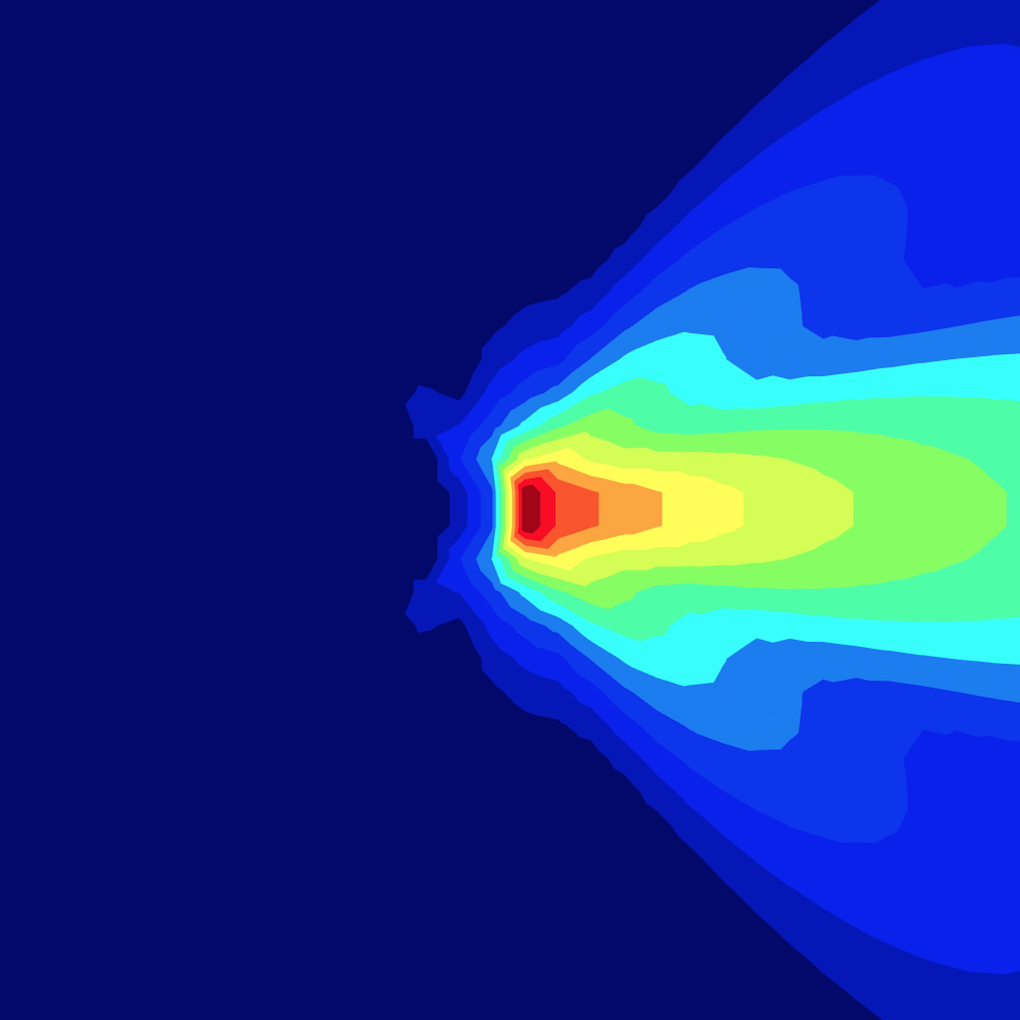
\includegraphics[scale=0.2]{archivos/130} & 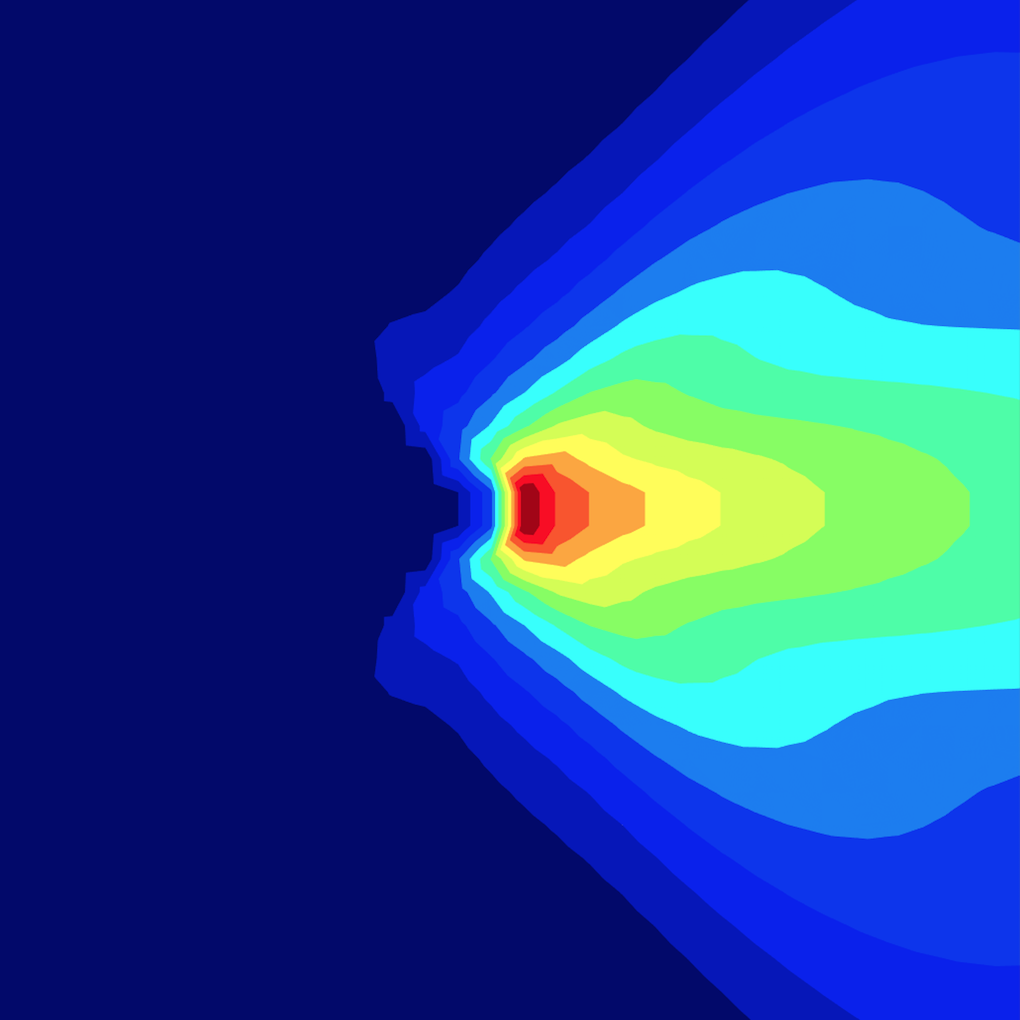
\includegraphics[scale=0.2]{archivos/160} & 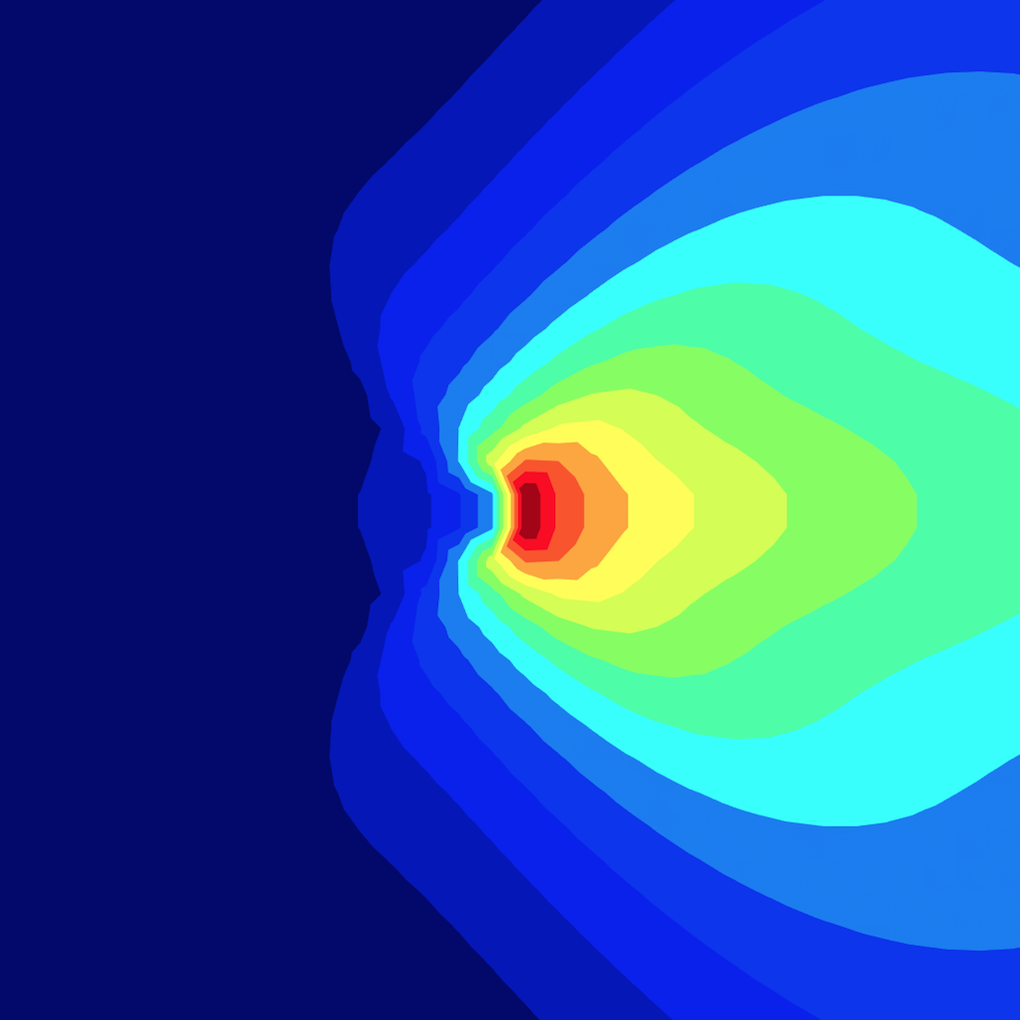
\includegraphics[scale=0.2]{archivos/190} \\
$Dist=1m \; ; \; \phi=30º$  & $Dist=1m \; ; \; \phi=60º$  & $Dist=1m \; ; \; \phi=90º$  \\
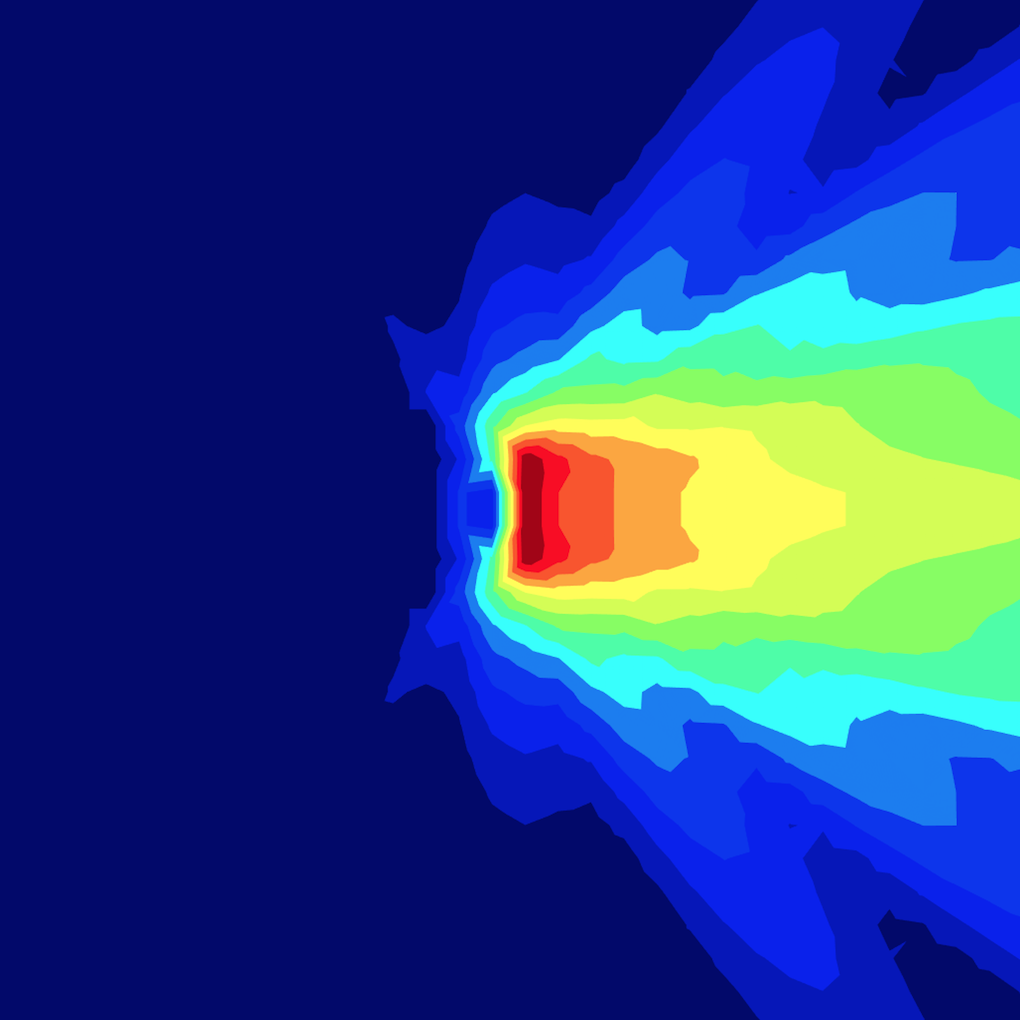
\includegraphics[scale=0.2]{archivos/230} & 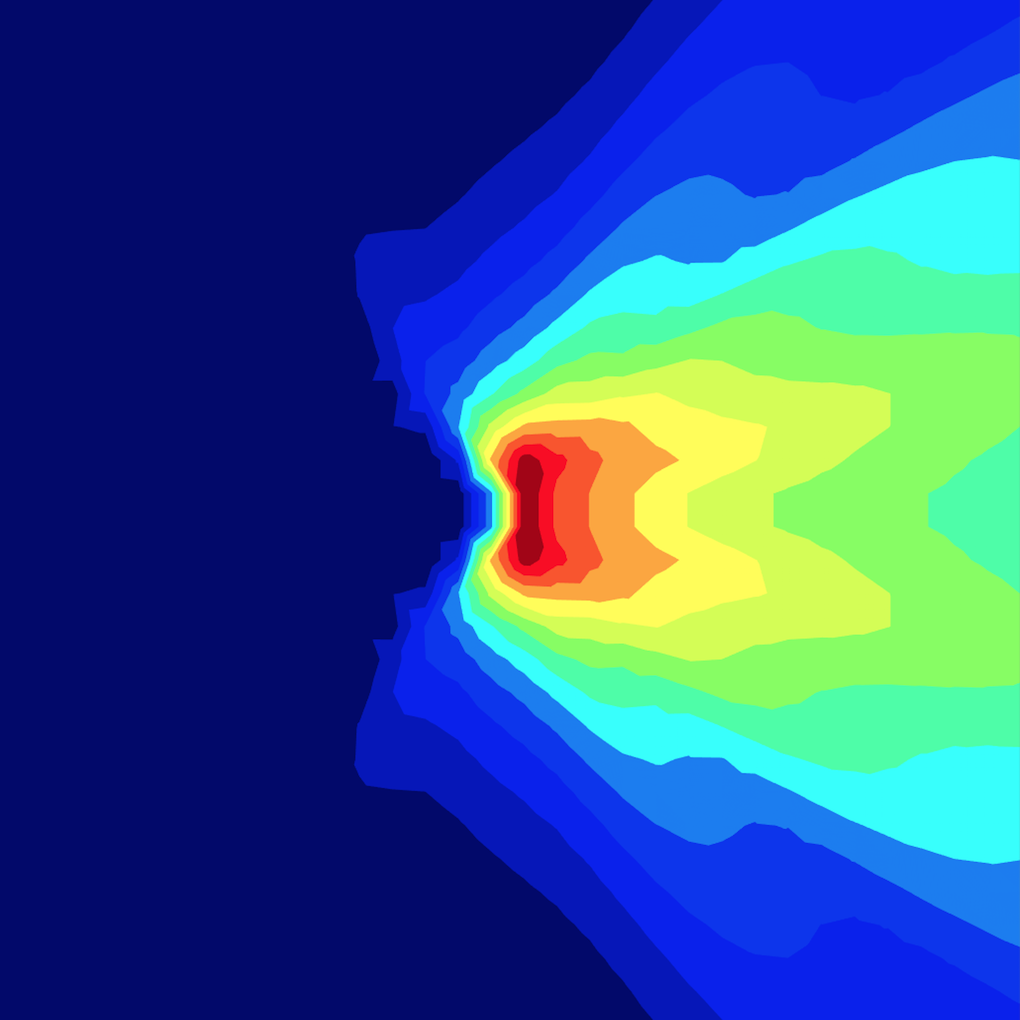
\includegraphics[scale=0.2]{archivos/260} & 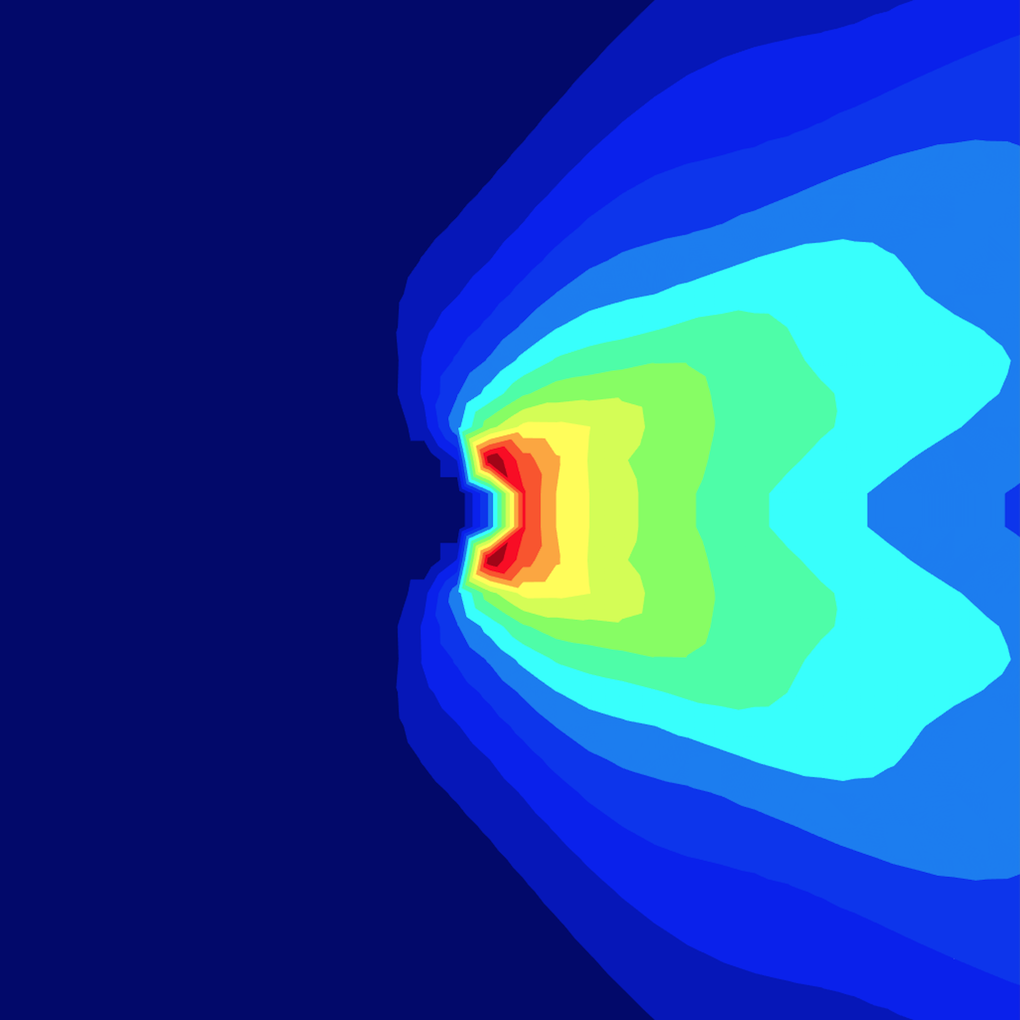
\includegraphics[scale=0.2]{archivos/290} \\
$Dist=2m \; ; \; \phi=30º$  & $Dist=2m \; ; \; \phi=60º$  & $Dist=2m \; ; \; \phi=90º$  \\
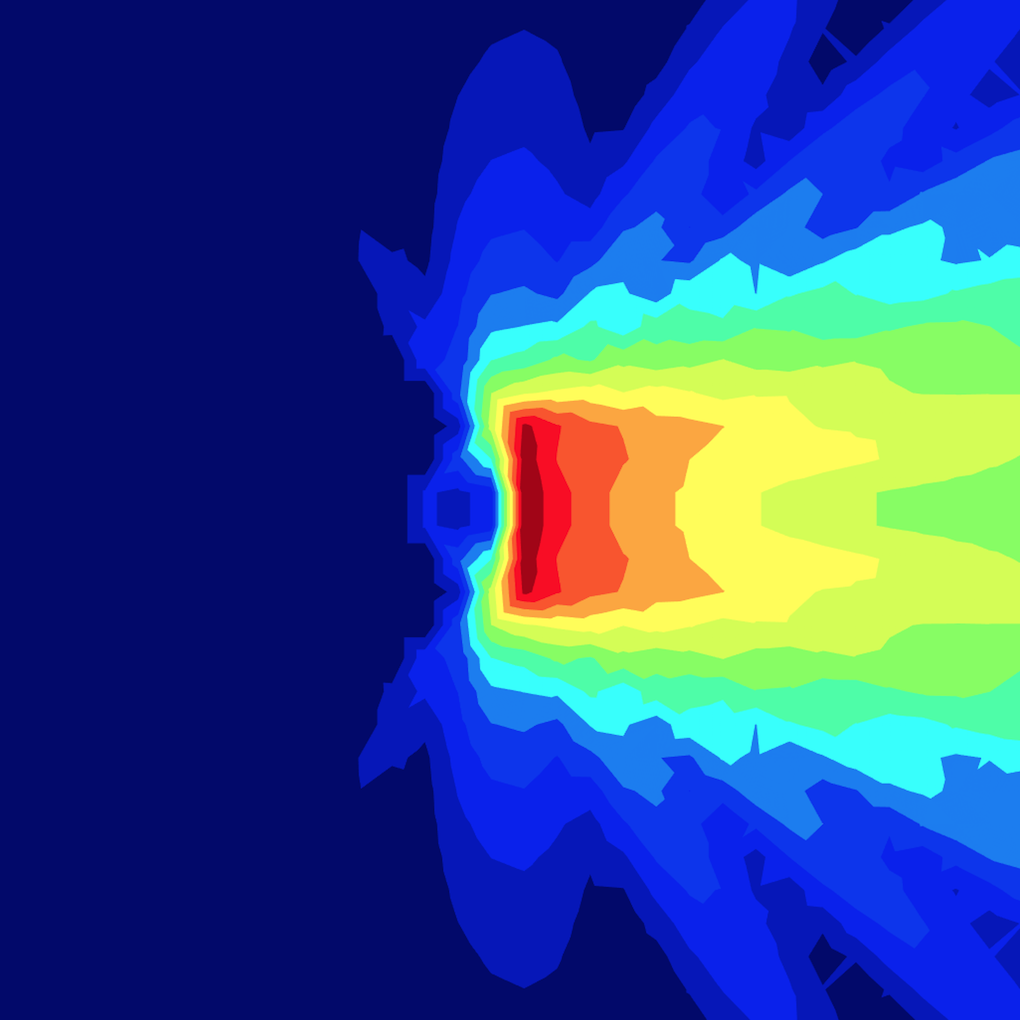
\includegraphics[scale=0.2]{archivos/330} & 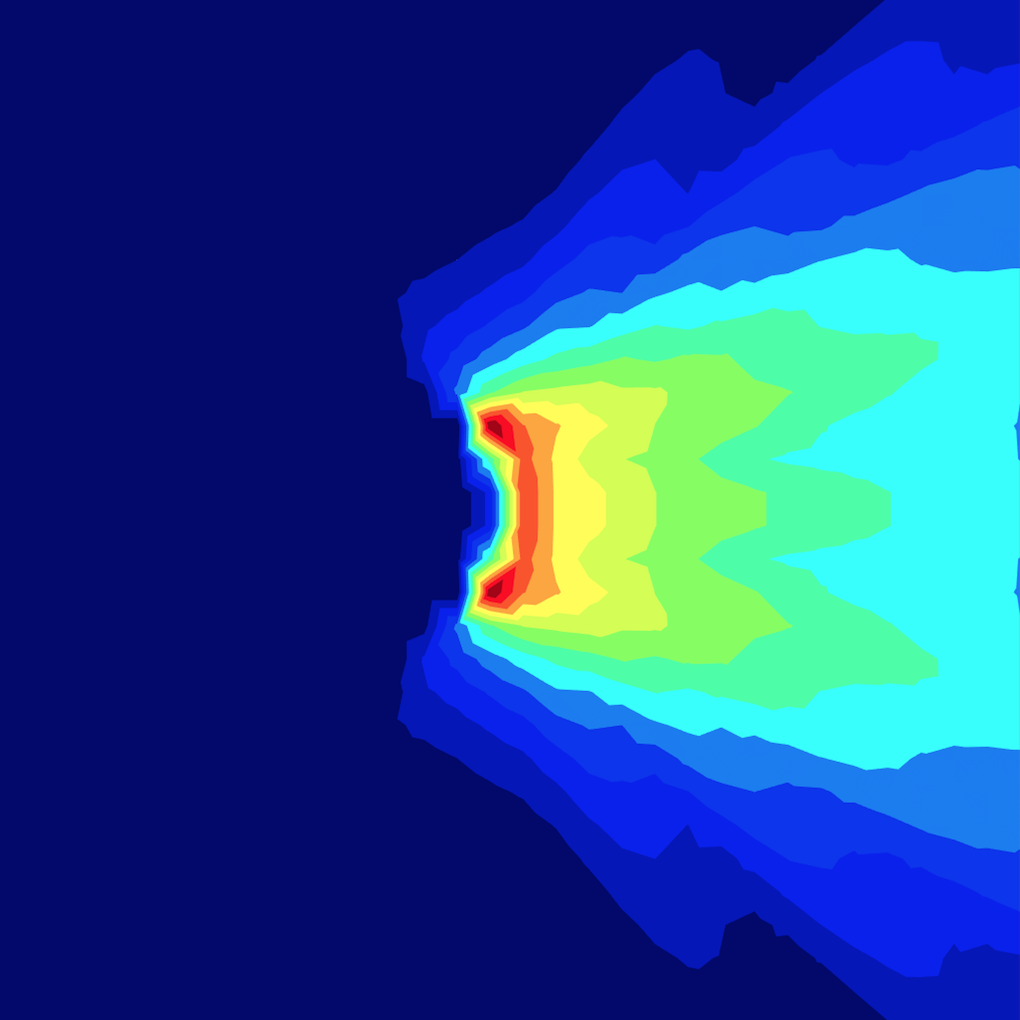
\includegraphics[scale=0.2]{archivos/360} & 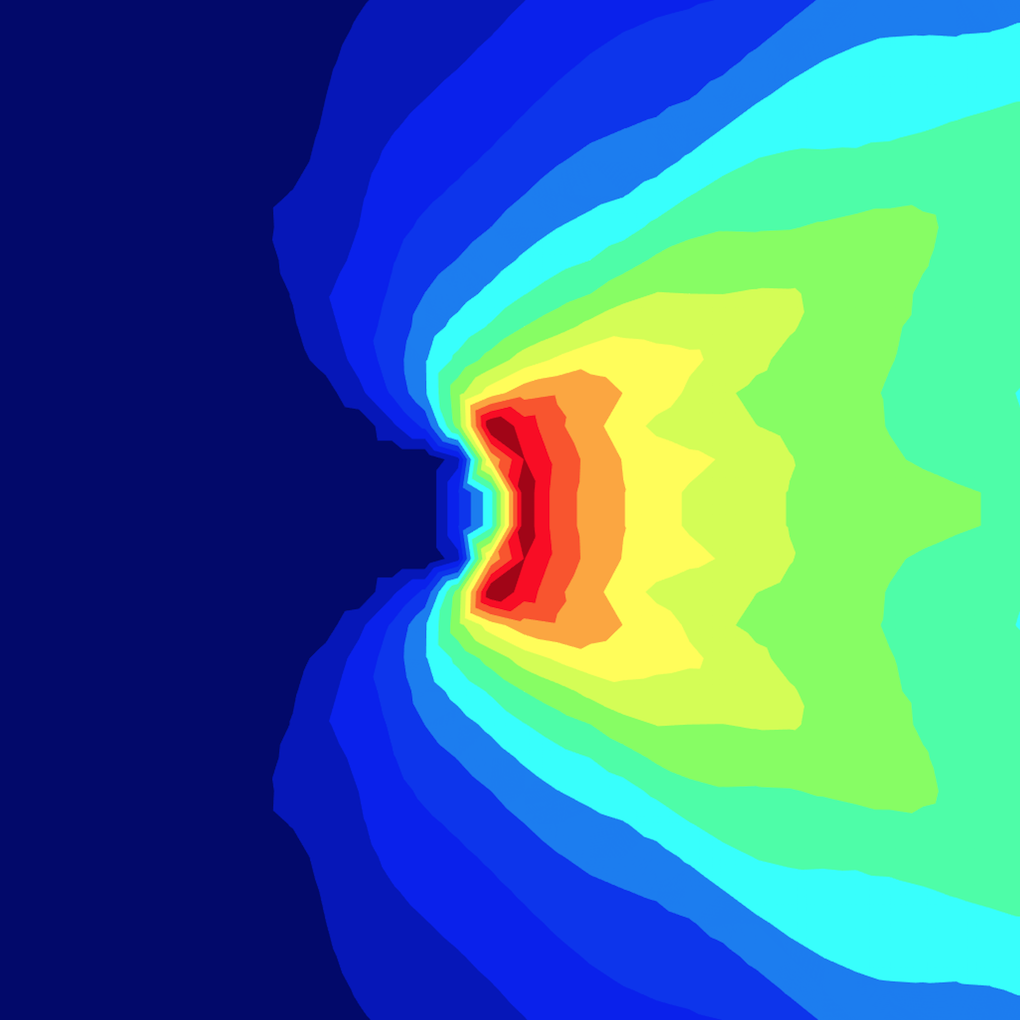
\includegraphics[scale=0.2]{archivos/390} \\
$Dist=3m \; ; \; \phi=30º$  & $Dist=3m \; ; \; \phi=60º$  & $Dist=3m \; ; \; \phi=90º$ \\
\end{tabular}
\caption{Esta es una tabla con múltiples imágenes. Útil cuando se deben mostrar varias juntas.}
\label{multiimagen} % 
\end{table}

Existe también la posibilidad de realizarlo sin tablas, con subfiguras:
\begin{lstlisting}[style=Latex-color]
\begin{figure}[h]
    \centering
    \begin{subfigure}[b]{0.4\textwidth} % Espacio horizontal ocupado por la subfigura
    	\centering
        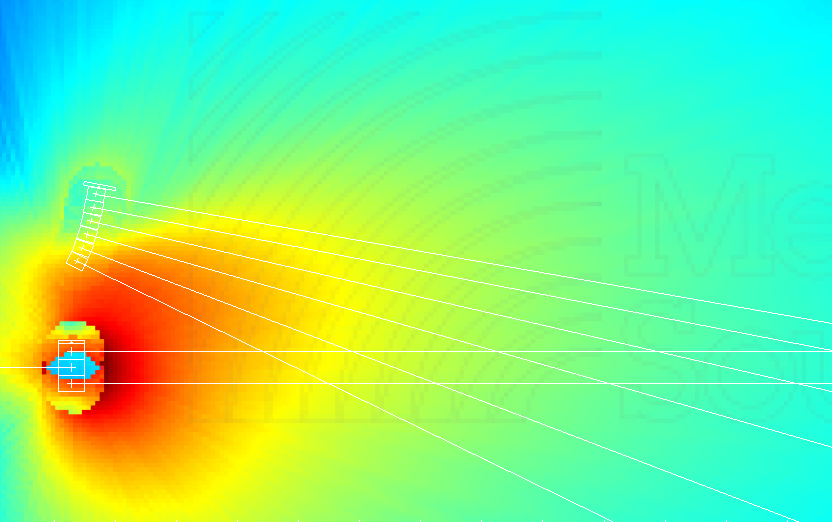
\includegraphics[width=4cm]{archivos/subs-sin} % Tamaño de la imagen
        \caption{Sin procesado.}
        \label{fig:gull}
    \end{subfigure}
    ~ % Añadir el espacio deseado, si se deja la linea en blanco la siguiente subfigura ira en una nueva linea
    \begin{subfigure}[b]{0.4\textwidth} % Espacio horizontal ocupado por la subfigura
    	\centering
        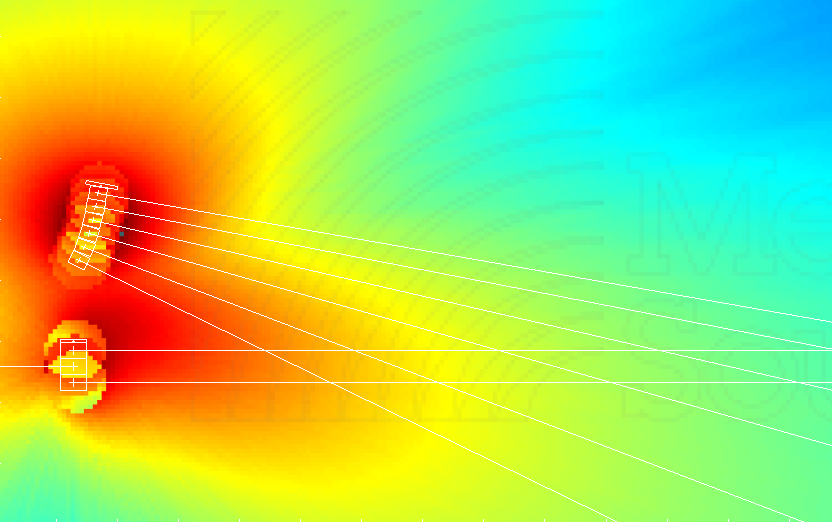
\includegraphics[width=4cm]{archivos/subs-con} % Tamaño de la imagen
        \caption{Con procesado.}
        \label{fig:tiger}
    \end{subfigure}
    \caption{Ejemplo de subfiguras}\label{sistemass}
\end{figure}
\end{lstlisting}
\begin{figure}[h]
    \centering
    \begin{subfigure}[b]{0.4\textwidth}
    	\centering
        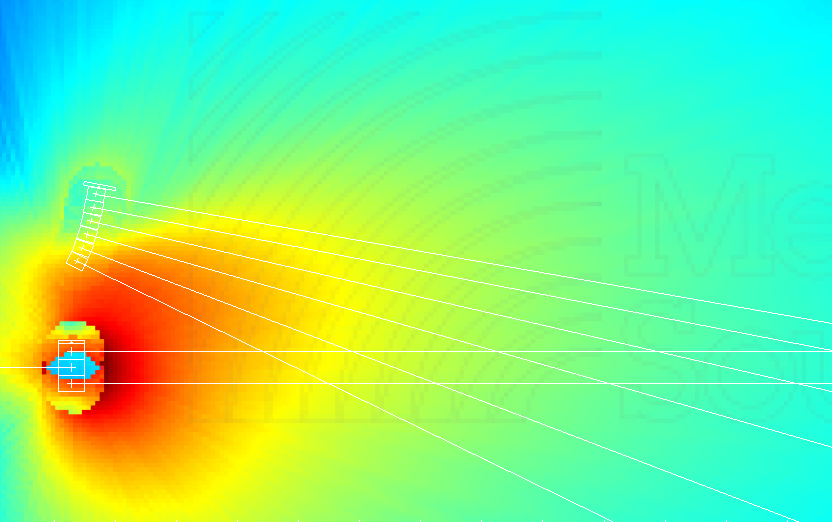
\includegraphics[width=4cm]{archivos/subs-sin}
        \caption{Sin procesado.}
        \label{fig:gull1}
    \end{subfigure}
    ~ % Añadir el espacio deseado, si se deja la linea en blanco la siguiente subfigura ira en una nueva linea
    \begin{subfigure}[b]{0.4\textwidth}
    	\centering
        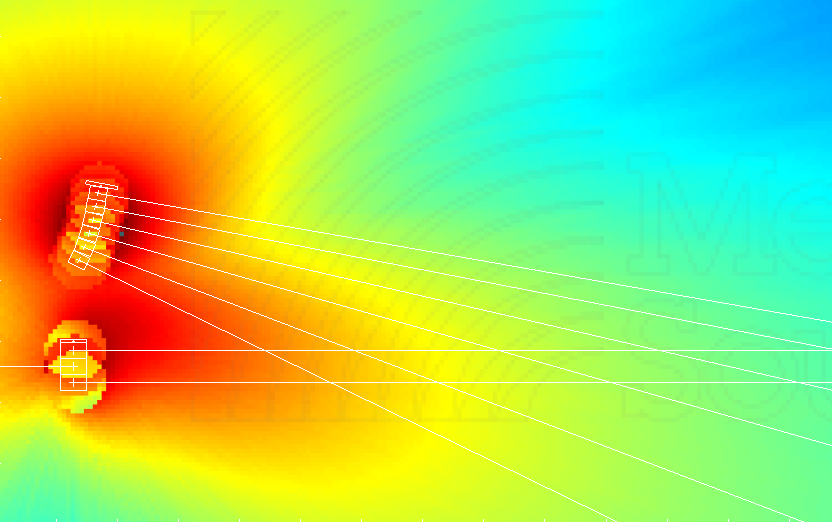
\includegraphics[width=4cm]{archivos/subs-con}
        \caption{Con procesado.}
        \label{fig:tiger1}
    \end{subfigure}
    \caption{Ejemplo de subfiguras}\label{sistemass1}
\end{figure}

\begin{figure}[h]
    \centering
    \begin{subfigure}[b]{\textwidth}
    	\centering
        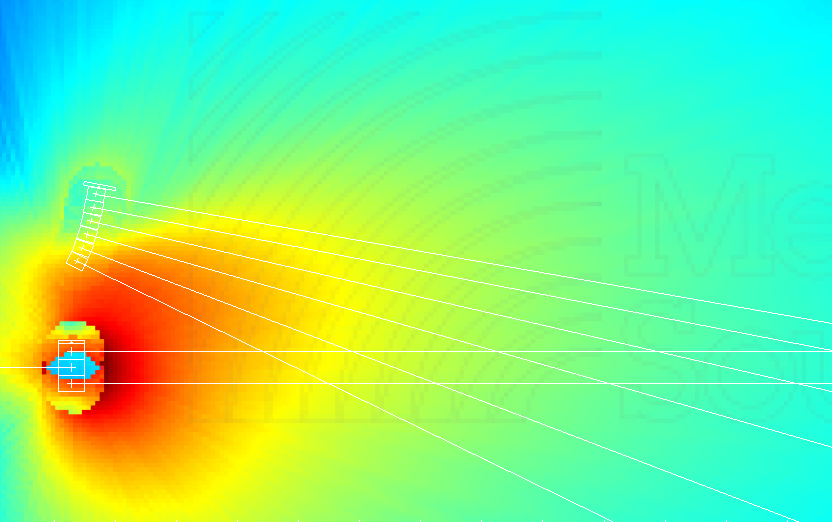
\includegraphics[width=4cm]{archivos/subs-sin}
        \caption{Sin procesado.}
        \label{fig:gull2}
    \end{subfigure}
    
    \begin{subfigure}[b]{\textwidth}
    	\centering
        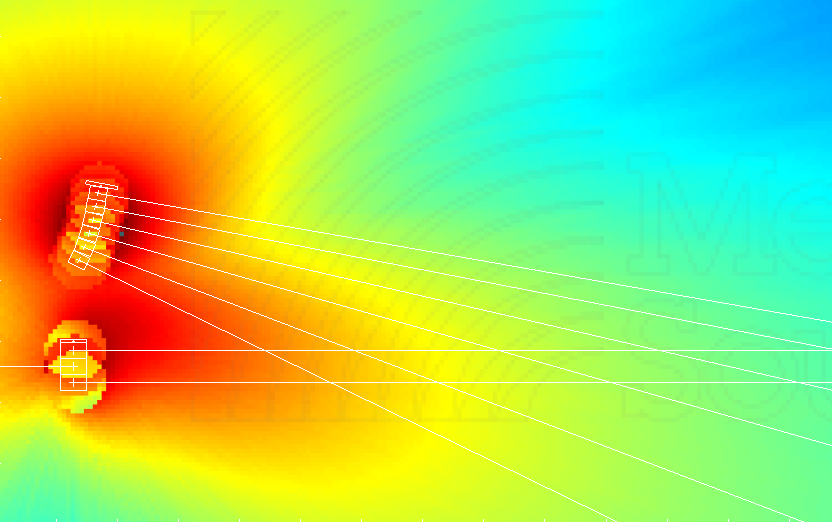
\includegraphics[width=4cm]{archivos/subs-con}
        \caption{Con procesado.}
        \label{fig:tiger2}
    \end{subfigure}
    \caption{Ejemplo de subfiguras vertical}\label{sistemass2}
\end{figure}

Si eliminas la línea '\textbackslash caption' de las subfiguras, tendrás las imágenes sin la información individual, aunque sí con la principal. Y obviamente, si eliminas el de la figura no se mostrará ninguna información.	% Plantilla: Se muestran figuras
%%%%%%%%%%%%%%%%%%%%%%%%%%%%%%%%%%%%%%%%%%%%%%%%%%%%%%%%%%%%%%%%%%%%%%%%
% Plantilla TFG/TFM
% Escuela Politécnica Superior de la Universidad de Alicante
% Realizado por: Jose Manuel Requena Plens
% Contacto: info@jmrplens.com / Telegram:@jmrplens
%%%%%%%%%%%%%%%%%%%%%%%%%%%%%%%%%%%%%%%%%%%%%%%%%%%%%%%%%%%%%%%%%%%%%%%%

\chapter{Desarrollo (Con ejemplos de código)}
\label{desarrollo}

\section{Inserción de código}
A veces tendrás que insertar algún pedazo de código fuente para explicar algo relacionado con él. No sustituyas explicaciones con códigos enormes. Si pones algo de código en tu TFG que sea para demostrar algo o explicar alguna solución.

\LaTeX~te ayuda a escribir código de manera que su presentación tenga las marcas y tabulaciones propias de este tipo de texto. Para ello, debes poner el código que escribas DENTRO de un entorno  que se llama ``listings''.  La plantilla ya tiene una serie de instrucciones para incluir el paquete ``listings'' y añadirle algunos modificadores por lo que no tienes que incluirlo tú. Simplemente, mete tu código en el entorno ``lstlisting'' y ya está. Puedes indicar el lenguaje en el que está escrito el código y así \LaTeX~lo mostrará mejor. 
\\
\par En el archivo \textit{estiloscodigoprogramacion.tex} están definidos algunos lenguajes para mostrarlos con un diseño concreto, se pueden modificar para cambiar el coloreado del código, qué términos se ponen en negrita, etc.
Si se quiere profundizar más en la función ``listings'' se puede consultar su manual en \url{http://osl.ugr.es/CTAN/macros/latex/contrib/listings/listings.pdf}, aunque hay mucha información en foros y blog's que es más fácil de comprender.

\par Veamos un ejemplo en la figura \ref{C_code}:

\begin{lstlisting}[style=Latex-color]
\begin{lstlisting}[style=C, caption={ejemplo código C},label=C_code]
	#include <stdio.h>
	int main(int argc, char* argv[]) {
  	puts("Hola mundo!");
	}
\ end{lstlisting}	
\end{lstlisting}

El resultado será:
\begin{lstlisting}[style=C, caption={ejemplo código C},label=C_code]
#include <stdio.h>
// Comentario
int main(int argc, char* argv[]) {
  puts("Hola mundo!");
}
\end{lstlisting}
\vspace{1em}
\noindent\hrule
\vspace{1em}
Si lo quieres en color, está definido el estilo C-color en el archivo \textit{estiloscodigoprogramacion.tex}, con algunos parámetros para mejorar la visualización:
\begin{lstlisting}[style=Latex-color]
\begin{lstlisting}[style=C-color, caption={ejemplo código C en color},label=C_code-color]
#include <stdio.h>
// Comentario
int main(int argc, char* argv[]) {
  puts("Hola mundo!");
}
\ end{lstlisting}
\end{lstlisting}
\begin{lstlisting}[style=C-color, caption={ejemplo código C en color},label=C_code-color]
	#include <stdio.h>
	// Comentario
	int main(int argc, char* argv[]) {
  	puts("Hola mundo!");
	}
\end{lstlisting}
\vspace{1em}
\noindent\hrule
\vspace{1em}
Por supuesto, puedes mejorar esta presentación utilizando más modificadores. En la sección \ref{usos} se indican algunos detalles.

Otro ejemplo, ahora para mostrar código PHP, sería escribir en tu fichero \LaTeX~lo siguiente:
\begin{lstlisting}[style=Latex-color,numbers=none]
 \begin{lstlisting}[style=PHP, caption={ejemplo código PHP},label=PHP_code]
 /* 
Ejemplo de código en PHP para escribir tu primer programa en este lenguaje
Copia este código en tu ordenador y ejecútalo
*/
<html>
  <head>
    <title>Prueba de PHP</title>
  </head>
  <body>
    <?php echo '<p>Hola Mundo</p>'; ?> //esto lo escribe TODO el mundo
  </body>
</html>
 \ end{lstlisting}
\end{lstlisting}
 
 y el resultado es el siguiente:
 
 \begin{lstlisting}[style=PHP, caption={ejemplo código PHP},label=PHP_code,firstnumber=100]
/* 
Ejemplo de código en PHP para escribir tu primer programa en este lenguaje. Copia este código en tu ordenador y ejecútalo
*/
 <html>
  <head>
    <title>Prueba de PHP</title>
  </head>
  <body>
    <?php echo '<p>Hola Mundo</p>'; ?> //esto lo escribe TODO el mundo
  </body>
</html>
 \end{lstlisting}
 \vspace{1em}
\noindent\hrule
\vspace{1em}
 O también en color: 
 \begin{lstlisting}[style=PHP-color, caption={ejemplo código PHP},label=PHP_code2]
/* 
Ejemplo de código en PHP para escribir tu primer programa en este lenguaje. Copia este código en tu ordenador y ejecútalo
*/
 <html>
  <head>
    <title>Prueba de PHP</title>
  </head>
  <body>
    <?php echo '<p>Hola Mundo</p>'; ?> //esto lo escribe TODO el mundo
  </body>
</html>
 \end{lstlisting}
 
 Observa cómo \LaTeX~ha puesto los comentarios en gris y ajustado el código para que se muestre más claro.
\vspace{1em}
\noindent\hrule
\vspace{1em}
 A continuación se muestran otros ejemplos:
 \begin{lstlisting}[style=Matlab-color, caption={ejemplo código Matlab en color},label=Matlab_code]
%% Code sections are highlighted.
% System command are supported...
!touch testFile.txt
A = [1, 2, 3;... %... as is line continuation.
     4, 5, 6];
fid = fopen('testFile.text', 'w');
for k=1:10
  fprintf(fid, '%6.2f \n', k)
end
x=1; %% this is just a comment, not the start of a section
% Context-sensitive keywords get highlighted correctly...
p = properties(person); %(here, properties is a function)
x = linspace(0,1,101);
y = x(end:-1:1);
% ... even in nonsensical code.
]end()()(((end while {    end    )end ))))end (end
%{
    block comments are supported
%} even
runaway block comments are
\end{lstlisting}

\begin{lstlisting}[style=Matlab, caption={ejemplo código Matlab en blanco y negro},label=Matlab_codebn]
%% Code sections are highlighted.
% System command are supported...
!touch testFile.txt
A = [1, 2, 3;... %... as is line continuation.
     4, 5, 6];
fid = fopen('testFile.text', 'w');
for k=1:10
  fprintf(fid, '%6.2f \n', k)
end
x=1; %% this is just a comment, not the start of a section
% Context-sensitive keywords get highlighted correctly...
p = properties(person); %(here, properties is a function)
x = linspace(0,1,101);
y = x(end:-1:1);
% ... even in nonsensical code.
]end()()(((end while {    end    )end ))))end (end
%{
    block comments are supported
%} even
runaway block comments are
\end{lstlisting}
\newpage
\begin{lstlisting}[style=Python-color, caption={ejemplo código Python en color}]
class Example (object):
    def __init__ (self, account, password):
        """e.g. account  = 'bob@example.com/test'
                password = 'bigbob'
        """

        reg = telepathy.client.ManagerRegistry()
        reg.LoadManagers()

        # get the gabble Connection Manager
        self.cm = cm = reg.GetManager('gabble')

        # get the parameters required to make a Jabber connection
        # begin ex.basics.dbus.language-bindings.python.methods.call
        cm[CONNECTION_MANAGER].RequestConnection('jabber',
            {
                'account':  account,
                'password': password,
            },
            reply_handler = self.request_connection_cb,
            error_handler = self.error_cb)
        # end ex.basics.dbus.language-bindings.python.methods.call
\end{lstlisting}

\begin{lstlisting}[style=Python, caption={ejemplo código Python en blanco y negro}]
class Example (object):
    def __init__ (self, account, password):
        """e.g. account  = 'bob@example.com/test'
                password = 'bigbob'
        """

        reg = telepathy.client.ManagerRegistry()
        reg.LoadManagers()

        # get the gabble Connection Manager
        self.cm = cm = reg.GetManager('gabble')

        # get the parameters required to make a Jabber connection
        # begin ex.basics.dbus.language-bindings.python.methods.call
        cm[CONNECTION_MANAGER].RequestConnection('jabber',
            {
                'account':  account,
                'password': password,
            },
            reply_handler = self.request_connection_cb,
            error_handler = self.error_cb)
        # end ex.basics.dbus.language-bindings.python.methods.call
\end{lstlisting}

\section{Usos y personalización}
\label{usos}

El texto que acompaña al código puedes incluirlo o no, también puedes decidir si el texto va numerado o no. A continuación se muestra como:
\begin{lstlisting}[style=Latex-color]
	% Con esta línea el código no tendrá título
	\begin{lstlisting}[style=Python]
		micodigo
	\ end{lstlisting}
\end{lstlisting}

\begin{lstlisting}[style=Python]
	micodigo
\end{lstlisting}
\vspace{1em}
\noindent\hrule
\vspace{1em}
\begin{lstlisting}[style=Latex-color]
	% Con esta línea el código tendrá el título abajo
	\begin{lstlisting}[style=Python, caption={Ejemplo de título abajo},captionpos=b]
		micodigo
	\ end{lstlisting}
\end{lstlisting}

\begin{lstlisting}[style=Python,caption={Ejemplo de título abajo},captionpos=b]
	micodigo
\end{lstlisting}
\vspace{1em}
\noindent\hrule
\vspace{1em}
\begin{lstlisting}[style=Latex-color]
	% Con esta línea el código tendrá título no numerado
	\begin{lstlisting}[style=Python, title={Ejemplo de título no numerado}]
		micodigo
	\ end{lstlisting}
\end{lstlisting}

\begin{lstlisting}[style=Python,title={Ejemplo de título no numerado}]
	micodigo
\end{lstlisting}
\vspace{1em}
\noindent\hrule
\vspace{1em}
\begin{lstlisting}[style=Latex-color]
	% Con esta línea el código no tendrá las líneas numeradas
\begin{lstlisting}[style=Python,numbers=none, title={Ejemplo de código sin número de líneas}]
	micodigo
	sin
	número
	de
	líneas
\ end{lstlisting}
\end{lstlisting}

\begin{lstlisting}[style=Python,numbers=none,title={Ejemplo de código sin número de líneas}]
		micodigo
		sin
		número
		de
		líneas
\end{lstlisting}

\section{Importar archivos fuente}

Existe la posibilidad de importar un archivo de código en lugar de copiar su contenido y pegarlo en \LaTeX.

Para realizarlo debes escribir:

\begin{lstlisting}[style=Latex-color]
\lstinputlisting[style=C++-color,caption={Archivo C++ importado}]{archivos/ejemplos/holamundo.cpp}	
\end{lstlisting}

Y se importará con el formato establecido entre los '[ ]':
\newpage
\lstinputlisting[style=C++-color,caption={Archivo C++ importado}]{archivos/ejemplos/holamundo.cpp}

A continuación se muestran otros ejemplos

\begin{lstlisting}[style=Latex-color]
\lstinputlisting[style=Python-color,caption={Archivo Py importado},label=importado_py]{archivos/ejemplos/holamundo.py}	
\end{lstlisting}

\lstinputlisting[style=Python-color,caption={Archivo Py importado},label=importado_py2]{archivos/ejemplos/holamundo.py}	

\begin{lstlisting}[style=Latex-color]
\lstinputlisting[style=Matlab-color,caption={Archivo Matlab importado},label=importado_m]{archivos/ejemplos/holamundo.m}	
\end{lstlisting}

\lstinputlisting[style=Matlab-color,caption={Archivo Matlab importado},label=importado_m]{archivos/ejemplos/holamundo.m}


		% Plantilla: Se muestran listados
%%%%%%%%%%%%%%%%%%%%%%%%%%%%%%%%%%%%%%%%%%%%%%%%%%%%%%%%%%%%%%%%%%%%%%%%
% Plantilla TFG/TFM
% Escuela Politécnica Superior de la Universidad de Alicante
% Realizado por: Jose Manuel Requena Plens
% Contacto: info@jmrplens.com / Telegram:@jmrplens
%%%%%%%%%%%%%%%%%%%%%%%%%%%%%%%%%%%%%%%%%%%%%%%%%%%%%%%%%%%%%%%%%%%%%%%%

\chapter{Resultados (Con ejemplos de gráficos)}
\label{resultados}

\section{Diagramas}
Gracias al paquete \textit{Tikz} se pueden incluir multitud de medios gráficos, diagramas, capas sobre imágenes, etc.
Existen múltiples formas de realizarlo, para ello es recomendable consultar la guía de iniciación disponible aquí: \url{http://cremeronline.com/LaTeX/minimaltikz.pdf} y también el manual completo disponible aquí: \url{http://osl.ugr.es/CTAN/graphics/pgf/base/doc/pgfmanual.pdf}.
\\
\par A continuación se muestran algunos ejemplos. Revisa el archivo .tex para ver cómo se utilizan.
\\
\par Imagen a la que se le ha añadido cuadros y texto desde latex:
\begin{figure}[ht]
\centering	
\resizebox{0.6\textwidth}{!}{%
\begin{tikzpicture}[x=39, y=47]%X,Y -> Corrección de coordenadas, según tamaño y posición de la imagen
    \node[anchor=south west,inner sep=0] (image) at (0,0) {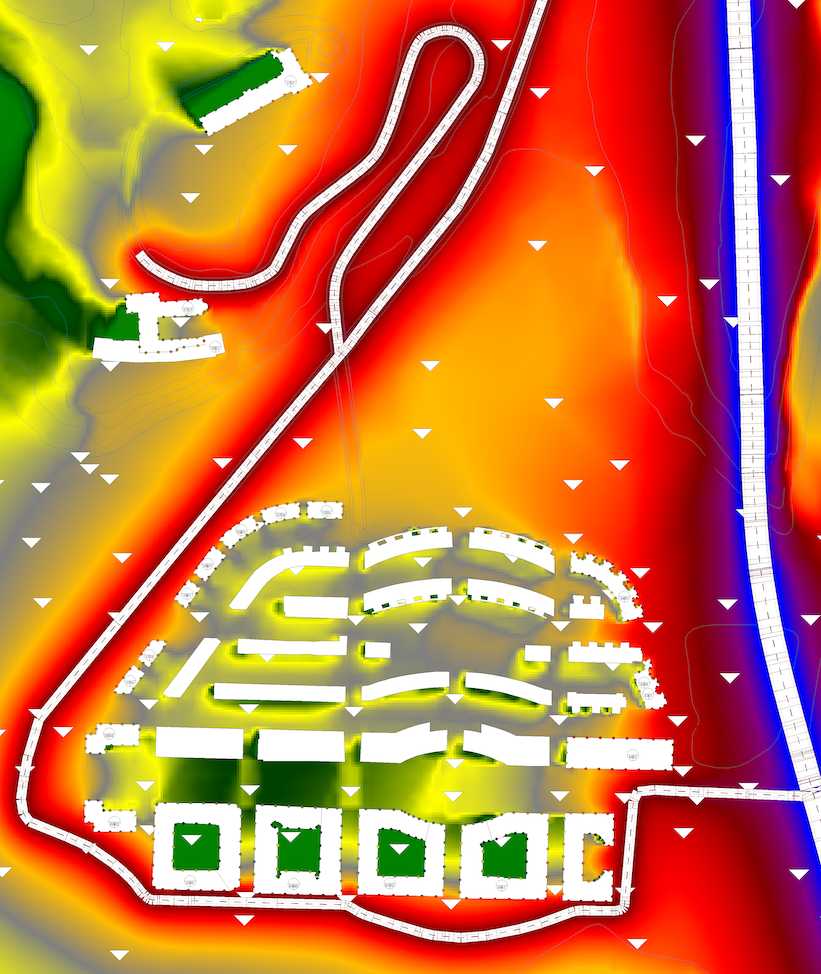
\includegraphics[width=0.9\textwidth]{archivos/mapadia}};
    % Imprimir coordenadas
    \begin{scope}[x={(image.south east)},y={(image.north west)}]
        \draw[help lines,xstep=.1,ystep=.1] (0,0) grid (1,1);
        \foreach \x in {0,1,...,9} { \node [anchor=north] at (\x/10,0) {\x}; }
        \foreach \y in {0,1,...,9} { \node [anchor=east] at (0,\y/10) {\y}; }
    \end{scope}
    % Residencias 1
    \draw[Caja1] (6.8,2) rectangle (8.3,4.5);
    \node[Texto2] at (6.8,2) {\textbf{Residencias 1}};
    % Residencias 2
    \draw[Caja1] (1,0.6) rectangle (7.6,1.8);
    \node[Texto2] at (1,0.6) {\textbf{Residencias 2}};
    % Residencias 3
    \draw[Caja1,rotate around={-45:(2.6,3.6)}] (2.6,3.6) ellipse (1cm and 3.1cm);
    \node[Texto2] at (1.2,2.1) {\textbf{Residencias 3}};
    % Hospital
    \draw[Caja1] (1,6) rectangle (3,7);
    \node[Texto2] at (1,6) {\textbf{Hospital}};
    % Colegio
    \draw[Caja1] (2.3,8.5) rectangle (3.9,9.5);
    \node[Texto2] at (2.3,8.5) {\textbf{Colegio}};
    % Numeros de edificios
    \node[Texto3,font=\tiny] at (7.5,4) {\textbf{1}};
    \node[Texto3,font=\tiny] at (7.9,2.9) {\textbf{2}};
    \node[Texto3,font=\tiny] at (7.7,2.3) {\textbf{3}};
    \node[Texto3,font=\tiny] at (7.2,1.2) {\textbf{4}};
    \node[Texto3,font=\tiny] at (6.2,1.2) {\textbf{5}};
    \node[Texto3,font=\tiny] at (4.9,1.2) {\textbf{6}};
    \node[Texto3,font=\tiny] at (3.6,1.2) {\textbf{7}};
    \node[Texto3,font=\tiny] at (2.4,1.2) {\textbf{8}};
    \node[Texto3,font=\tiny] at (1.5,1.7) {\textbf{9}};
    \node[Texto3,font=\tiny] at (1.5,2.5) {\textbf{10}};
    \node[Texto3,font=\tiny] at (1.5,3) {\textbf{11}};
    \node[Texto3,font=\tiny] at (1.8,3.4) {\textbf{12}};
    \node[Texto3,font=\tiny] at (2.2,3.8) {\textbf{13}};
    \node[Texto3,font=\tiny] at (2.5,4.2) {\textbf{14}};
    \node[Texto3,font=\tiny] at (3,4.5) {\textbf{15}};
    \node[Texto3,font=\tiny] at (3.4,4.8) {\textbf{16}};
    \node[Texto3,font=\tiny] at (4,4.8) {\textbf{17}};
    % Nombres de carreteras
    \node[Texto3] at (9.2,7) {\textbf{A-7}};
    \node[Texto3] at (9,1.8) {\textbf{N-1}};
    \node[Texto3] at (4,8) {\textbf{N-2}};
\end{tikzpicture}
}
\end{figure}

En muchas ocasiones es necesario realizar un diagrama de bloques, más abajo se muestra un ejemplo de ello. En la red hay multitud de ejemplos que pueden ser fácilmente modificables para un fin concreto, como por ejemplo en esta web: \url{http://www.texample.net/tikz/examples/tag/block-diagrams/}.
\begin{figure}[ht]
\centering 
\begin{tikzpicture}[node distance=2cm, auto]
	% Cuadros
	\node (pc) [rectvioleta,text width=3cm] {Ordenador{\\}\small{Software: ARTA} \par};
	\node (sound) [rectamarillo, below of=pc, text width=4cm] {Tarjeta de sonido {\\}Tascam US-144MKII \par};
	\node (nexus) [rectverde, right of=sound,xshift=6cm, text width=8cm] { Amplificador/Adaptador de impedancia{\\}DIY\par };
	\node (acel) [rectnaranja, below of=nexus,text width=3cm,xshift=0cm]{\small Acelerómetro {\\}Brüel {\&} Kjær TYPE 4514B-002 \par};
	\node (micro) [rectnaranja, below of=sound,text width=3cm,xshift=0cm]{\small Micrófono {\\}Behringer ECM8000 \par};
	\node (excit) [rectnaranja, below of=acel,text width=3cm,xshift=2cm]{\small Excitador \par};
	\node(barra) [romborosa, below of=acel,xshift=-3.1cm]{\small Barra \par};
	% Flechas
	\draw[arrow] (pc) -- (sound);
	\draw[arrow] (sound) -- (pc);
	\draw[arrow] (nexus) -- (sound);
	\draw[arrow] (excit) -- (barra.east);
	\draw[arrow] (micro) -- (sound);
	\draw[arrow] (barra.west) -- (0,-6)-- (micro.south);
	\draw[arrow] (barra.west) -- (3.4,-4)--(acel.west);
 	\draw[arrow] (acel) -- (nexus);	
\end{tikzpicture}
\caption{Diagrama realizado en latex con Tikz.}
\label{fig:blockcv}
\end{figure}



\section{Gráficas}

Existen múltiples formas de generar gráficas para latex. Hay disponibles herramientas como GeoGebra que dispone de la utilidad para exportar los gráficos en formato Tkiz. También funciones para Matlab que genera las gráficas que muestra habitualmente pero en código para Tkiz.

\subsection{Línea}
La forma más simple, aunque no sencilla cuando abarca muchos datos es la siguiente:

\begin{lstlisting}[style=Latex-color]
\begin{figure}[ht]
\centering
	\begin{tikzpicture}
  		\begin{axis}
  			[ymin=0,ymax=5, % Límites del eje y
  			xmin=0,xmax=6,  % Límites del eje x
  			ylabel= eje Y, 	% Nombre del eje y
    		xlabel= eje X]  % Nombre del eje x
    		\addplot+[smooth] coordinates % Une los puntos curva suavizada
      		{(0,0) (1,2) (2,3 (4,3))}; % Puntos de la gráfica
  		\end{axis}
	\end{tikzpicture}
\caption{Gráfica sencilla.}
\end{figure}
\end{lstlisting}

El resultado es el siguiente:
\\
\begin{figure}[ht]
\centering
	\begin{tikzpicture}
  		\begin{axis}
  			[ymin=0,ymax=5, 
  			xmin=0,xmax=6,
  			ylabel= eje Y,
    		xlabel= eje X]
    		\addplot+[smooth] coordinates
      		{(0,0) (1,2) (2,3) (4,3)};
  		\end{axis}
	\end{tikzpicture}
\caption{Gráfica sencilla.}
\end{figure}
\FloatBarrier

Otro ejemplo, en este caso las lineas están calculadas directamente en LaTex y después cada una tiene una anotación (el código se encuentra en el archivo archivos/ejemplos/perjudicialesopticacentro.tex):

\begin{figure}[H]
	\centering%
    %%%%%%%%%%%%%%%%%%%%%%%%%%%%%%%%%%%%%%%%%%%%%%%%%%%%%%%%%%%%%%%%%%%%%%%%
% Escuela Politécnica Superior de la Universidad de Alicante
% Realizado por: Jose Manuel Requena Plens
% Contacto: info@jmrplens.com / Telegram:@jmrplens
%%%%%%%%%%%%%%%%%%%%%%%%%%%%%%%%%%%%%%%%%%%%%%%%%%%%%%%%%%%%%%%%%%%%%%%%

\definecolor{mycolor1}{rgb}{1.00000,0.00000,1.00000}%
%
\begin{tikzpicture}

\begin{axis}[%
width=0.5\textwidth,
height=0.3\textwidth,
at={(0\textwidth,0\textwidth)},
scale only axis,
xmin=0,
xmax=24,
xlabel style={font=\color{white!15!black}},
xlabel={Distancia (m)},
ymin=68,
ymax=84,
ytick distance=2,
axis y line=left,
axis x line=bottom,
cycle list name=color list,
ylabel style={font=\color{white!15!black}},
ylabel={Nivel de presión acústica (dB)},
axis background/.style={fill=white},
legend style={legend cell align=left, align=left, draw=white!15!black}
]

% Campos utiles

% 1
\addplot+[ line width=1.5,domain=0.5:9.14, samples=10,every node/.style={xshift=-4pt}]
{10*log10(1.0337e+12 * ( (4*0.0026389378)/(512*(-ln(1-0.1176))) * e^(-(13.82*((x/343)+0.05)*1.195 / 1.24))*1.175))} node [pos=1,pin=0:{\tiny{495 $m^3$}}] {};

% 1.2
\addplot+[ line width=1.5,domain=0.5:10.97, samples=10,every node/.style={xshift=-4pt}]
{10*log10(1.0337e+12 * ( (4*0.0026389378)/(737*(-ln(1-0.1176))) * e^(-(13.82*((x/343)+0.05)*1.309 / 1.24))*1.168))} node [pos=1,pin=0:{\tiny{855 $m^3$}}] {};

% 1.5
\addplot+[ line width=1.5,domain=0.5:13.71, samples=10,every node/.style={xshift=-4pt}]
{10*log10(1.0337e+12 * ( (4*0.0026389378)/(1152*(-ln(1-0.1176))) * e^(-(13.82*((x/343)+0.05)*1.373 / 1.24))*1.101))} node [pos=1,pin=0:{\tiny{1670 $m^3$}}] {};

%% 1.7
\addplot[line width=1.5,color=teal, domain=0.5:15.54, samples=10,every node/.style={xshift=-4pt}]
{10*log10(1.0337e+12 * ( (4*0.0026389378)/(1479*(-ln(1-0.1176))) * e^(-(13.82*((x/343)+0.05)*1.422 / 1.24))*1.074))} node [pos=1,pin=0:{\tiny{2431 $m^3$}}] {};

% 20
\addplot+[ line width=1.5,domain=0.5:18.27, samples=10,every node/.style={xshift=-4pt}]
{10*log10(1.0337e+12 * ( (4*0.0026389378)/(2048*(-ln(1-0.1176))) * e^(-(13.82*((x/343)+0.05)*1.486 / 1.24))*1.045))} node [pos=1,pin=0:{\tiny{3958 $m^3$}}] {};


\end{axis}
\end{tikzpicture}%



%
    \caption{OP/S003}%
\end{figure}%

\subsection{Barras}
Otro ejemplo es la gráfica de barras:
\begin{lstlisting}[style=Latex-color]
\begin{figure}[ht]
\centering
\begin{tikzpicture}
	\begin{axis}[
	    ybar=12pt,
	    ymin=0,ymax=150,
	    xtick=data,
	    enlarge x limits={abs=2cm},
	    symbolic x coords={rubio, moreno},
	    bar width = 20pt,
	    ylabel= número,
	    xlabel= color de pelo,
	        ytick align=outside,
	        ytick pos=left,
	        major x tick style = transparent,
	        legend style={at={(0.04,0.96)},anchor=north west, font=\footnotesize, legend cell align=left,},
	        ]
	    \addplot[ybar,fill=blue, area legend] coordinates {
	        (rubio,20)
	        (moreno,100)};
	    \addplot[ybar,fill=purple, area legend] coordinates {
	        (rubio,110)
	        (moreno,105)};
	 \legend{Chicos, Chicas}
	\end{axis}
\end{tikzpicture}
\caption{Gráfica barras.}
\end{figure}
\end{lstlisting}

El resultado es el siguiente:

\begin{figure}[ht]
\centering
\begin{tikzpicture}
	\begin{axis}[
	    ybar=12pt,
	    ymin=0,ymax=150,
	    xtick=data,
	    enlarge x limits={abs=2cm},
	    symbolic x coords={rubio, moreno},
	    bar width = 20pt,
	    ylabel= número,
	    xlabel= color de pelo,
	        ytick align=outside,
	        ytick pos=left,
	        major x tick style = transparent,
	        legend style={at={(0.04,0.96)},anchor=north west, font=\footnotesize, legend cell align=left,},
	        ]
	    \addplot[ybar,fill=blue, area legend] coordinates {
	        (rubio,20)
	        (moreno,100)};
	    \addplot[ybar,fill=purple, area legend] coordinates {
	        (rubio,110)
	        (moreno,105)};
	 \legend{Chicos, Chicas}
	\end{axis}
\end{tikzpicture}
\caption{Gráfica barras.}
\end{figure}
\FloatBarrier

\subsection{Polar}
Un ejemplo de gráfica polar semicircular (ver archivo archivos/ejemplos/polarnorm.tex):

\begin{figure}[H]
    	\centering%
         {\scalefont{0.8}%
    %%%%%%%%%%%%%%%%%%%%%%%%%%%%%%%%%%%%%%%%%%%%%%%%%%%%%%%%%%%%%%%%%%%%%%%%
% Plantilla TFG/TFM
% Escuela Politécnica Superior de la Universidad de Alicante
% Realizado por: Jose Manuel Requena Plens
% Contacto: info@jmrplens.com / Telegram:@jmrplens
%%%%%%%%%%%%%%%%%%%%%%%%%%%%%%%%%%%%%%%%%%%%%%%%%%%%%%%%%%%%%%%%%%%%%%%%


\begin{tikzpicture}
\begin{polaraxis}[
	width=0.7\textwidth,
	height=0.7\textwidth,
   	ymin=-24,ymax=0,
   	xmin=-90,xmax=90,
   	xtick={-90,-75,...,90},
   	ytick={-24,-18,...,0},
   	minor y tick num=1,
   	ytick style={yshift=-4.63cm},
   	xticklabel=$\pgfmathprintnumber{\tick}^\circ$,
   	xticklabel style={inner xsep=1pt,ellipse,anchor=\tick-90},
   	yticklabel style={xshift=-0.3cm,yshift=-0.3cm},
   	rotate=90,
   	y coord trafo/.code=\pgfmathparse{#1+24},
   	y coord inv trafo/.code=\pgfmathparse{#1-24},
  	ylabel={Atenuación (dBV)},
   	y label style={at={(0.42,-0.3)}},
    every axis legend/.append style={at={(1.2,0)},anchor=north},
   	legend columns=4,
   	cycle list name=color list,
  	grid=both,
]
%%%%
% DATOS
%%%%

% 125 Hz
\addplot+ [no markers, thick] table [row sep=crcr] {
-90	-1.72467814939056\\
-80	-1.39502194748928\\
-70	-1.21429283845364\\
-60	-1.00637477945158\\
-50	-0.840171759843390\\
-40	-0.513117825581858\\
-30	-0.312245425134396\\
-20	-0.174766911961633\\
-10	-0.0693431271095548\\
0	0\\
10	-0.0693431271095548\\
20	-0.174766911961633\\
30	-0.312245425134396\\
40	-0.513117825581858\\
50	-0.840171759843390\\
60	-1.00637477945158\\
70	-1.21429283845364\\
80	-1.39502194748928\\
90	-1.72467814939056\\
};
\addlegendentry{125 Hz}

% 250 Hz
\addplot+ [no markers, thick] table [row sep=crcr] {
-90	-2.93647985014495\\
-80	-2.58924713825609\\
-70	-2.07154743573673\\
-60	-1.58004347746668\\
-50	-1.18692289277002\\
-40	-0.831096645385170\\
-30	-0.520252849633241\\
-20	-0.290340966177958\\
-10	-0.125751595259928\\
0	0\\
10	-0.125751595259928\\
20	-0.290340966177958\\
30	-0.520252849633241\\
40	-0.831096645385170\\
50	-1.18692289277002\\
60	-1.58004347746668\\
70	-2.07154743573673\\
80	-2.58924713825609\\
90	-2.93647985014495\\
};
\addlegendentry{250 Hz}

% 500 Hz
\addplot+ [no markers, thick] table [row sep=crcr] {
-90	-6.09247981547998\\
-80	-4.92970035404602\\
-70	-3.94022779907609\\
-60	-3.04724262203246\\
-50	-2.20250965801318\\
-40	-1.51751670631493\\
-30	-0.901656083415322\\
-20	-0.430295873745550\\
-10	-0.137302043547450\\
0	0\\
10	-0.137302043547450\\
20	-0.430295873745550\\
30	-0.901656083415322\\
40	-1.51751670631493\\
50	-2.20250965801318\\
60	-3.04724262203246\\
70	-3.94022779907609\\
80	-4.92970035404602\\
90	-6.09247981547998\\
};
\addlegendentry{500 Hz}

% 1000 Hz
\addplot+ [no markers, thick] table [row sep=crcr] {
-90	-7.56789211935512\\
-80	-6.62816595706798\\
-70	-5.52277371644042\\
-60	-4.33467545812354\\
-50	-3.13339535257511\\
-40	-2.05909345347580\\
-30	-1.17203420486137\\
-20	-0.523179334693538\\
-10	-0.128596775989607\\
0	0\\
10	-0.128596775989607\\
20	-0.523179334693538\\
30	-1.17203420486137\\
40	-2.05909345347580\\
50	-3.13339535257511\\
60	-4.33467545812354\\
70	-5.52277371644042\\
80	-6.62816595706798\\
90	-7.56789211935512\\
};
\addlegendentry{1 kHz}

% 2000 Hz
\addplot+ [no markers, thick] table [row sep=crcr] {
-90	-14.4940605430080\\
-80	-12.7515170649147\\
-70	-10.9391538310668\\
-60	-9.13813062972114\\
-50	-7.31396133207484\\
-40	-5.44124573776644\\
-30	-3.54658907253479\\
-20	-1.91024948494566\\
-10	-0.704464176648823\\
0	0\\
10	-0.704464176648823\\
20	-1.91024948494566\\
30	-3.54658907253479\\
40	-5.44124573776644\\
50	-7.31396133207484\\
60	-9.13813062972114\\
70	-10.9391538310668\\
80	-12.7515170649147\\
90	-14.4940605430080\\
};
\addlegendentry{2 kHz}

% 4000 Hz
\addplot+ [no markers, thick] table [row sep=crcr] {
-90	-20.8595379753136\\
-80	-19.5111125476763\\
-70	-17.5530334315451\\
-60	-15.1562865020723\\
-50	-12.6153094614475\\
-40	-9.78583047231908\\
-30	-6.34807022561957\\
-20	-3.07890709456410\\
-10	-0.920648439706582\\
0	0\\
10	-0.920648439706582\\
20	-3.07890709456410\\
30	-6.34807022561957\\
40	-9.78583047231908\\
50	-12.6153094614475\\
60	-15.1562865020723\\
70	-17.5530334315451\\
80	-19.5111125476763\\
90	-20.8595379753136\\
};
\addlegendentry{4 kHz}

% 8000 Hz
\addplot+ [no markers, thick] table [row sep=crcr] {
-90	-19.8608838454044\\
-80	-17.8504412710498\\
-70	-14.6995990848335\\
-60	-12.7200970148256\\
-50	-10.7405694231973\\
-40	-8.26676493005069\\
-30	-4.30385837835709\\
-20	-2.28439452050384\\
-10	-1.25666726464311\\
0	0\\
10	-1.25666726464311\\
20	-2.28439452050384\\
30	-4.30385837835709\\
40	-8.26676493005069\\
50	-10.7405694231973\\
60	-12.7200970148256\\
70	-14.6995990848335\\
80	-17.8504412710498\\
90	-19.8608838454044\\
};
\addlegendentry{8 kHz}

% 16000 Hz
\addplot+ [no markers, thick] table [row sep=crcr] {
-90	-13.2702037690998\\
-80	-13.0567210721723\\
-70	-11.6584528874959\\
-60	-10.0279714036086\\
-50	-9.30230549595443\\
-40	-5.30129835593380\\
-30	-5.79648449690136\\
-20	-6.18064845743399\\
-10	-3.22991472126657\\
0	0\\
10	-3.22991472126657\\
20	-6.18064845743399\\
30	-5.79648449690136\\
40	-5.30129835593380\\
50	-9.30230549595443\\
60	-10.0279714036086\\
70	-11.6584528874959\\
80	-13.0567210721723\\
90	-13.2702037690998\\
};
\addlegendentry{16 kHz}


\end{polaraxis}

\end{tikzpicture}%%
    }
    \caption{Directividad normalizada del altavoz (0 dBV en el eje).}\label{norma}
\end{figure}


\section{Importados de MATLAB}
\label{impmatlab}
Gracias a la herramienta \textit{matlab2tikz} (\url{https://es.mathworks.com/matlabcentral/fileexchange/22022-matlab2tikz-matlab2tikz}) se pueden exportar las gráficas de cualquier tipo de Matlab a latex.
Después de incluir los archivos de \textit{matlab2tikz} se debe escribir una llamada después de crear la figura tal que:

\begin{lstlisting}[style=Matlab-color,caption={Ejemplo de llamada a matlab2tikz}]
fig = plot(x,y);
matlab2tikz('figurehandle',fig,'NombreArchivo.tex','height','5cm','width','13.5cm','strict',true,'showHiddenStrings',true,'showInfo',false)
\end{lstlisting}

Y para utilizar el archivo generado por la función en este documento:
\begin{lstlisting}[style=Latex-color]
\begin{figure}[ht]
	\centering
	{\scalefont{0.8}% This file was created by matlab2tikz.
%
\definecolor{mycolor1}{rgb}{0.00000,1.00000,1.00000}%
%
\begin{tikzpicture}

\begin{axis}[%
width=12.837cm,
height=5cm,
at={(0cm,0cm)},
scale only axis,
separate axis lines,
every outer x axis line/.append style={white!15!black},
every x tick label/.append style={font=\color{white!15!black}},
every x tick/.append style={white!15!black},
xmode=log,
xmin=15.625,
xmax=20158.736798318,
xtick={15.75,31.5,63,125,250,500,1000,2000,4000,8000,16000,24000},
xticklabels={{15.75},{31.5},{63},{125},{250},{500},{1000},{2000},{4000},{8000},{16000},{24000}},
xminorticks=true,
minor x tick num={3},
xlabel style={font=\color{white!15!black}},
xlabel={Frecuencia (Hz)},
every outer y axis line/.append style={white!15!black},
every y tick label/.append style={font=\color{white!15!black}},
every y tick/.append style={white!15!black},
ymin=-76.8103540908063,
ymax=7.89608497583378,
ytick={-70,-60,-50,-40,-30,-20,-10,0},
ylabel style={font=\color{white!15!black}},
ylabel={Amplitud (dBV)},
axis background/.style={fill=white},
xmajorgrids,
xminorgrids,
ymajorgrids,
grid style={solid},
minor grid style={dotted},
legend style={at={(0.03,0.97)}, anchor=north west, legend cell align=left, align=left, draw=white!15!black}
]
\addplot [color=blue, line width=0.5pt]
  table[row sep=crcr]{%
15.625	-59.82445\\
16.554110849364	-60.5623842620438\\
17.538469504834	-61.8453599337536\\
18.5813611719175	-63.5771407909652\\
19.6862664046074	-65.4392\\
20.8568727214068	-64.7401066715843\\
22.0970869120796	-63.8280672771138\\
23.4110480761981	-62.4796867506898\\
24.8031414370031	-57.5235393587445\\
26.2780129766786	-57.1510284649747\\
27.8405849418856	-56.1120339592741\\
29.4960722713029	-51.4584375460028\\
31.25	-43.9775628086098\\
33.108221698728	-43.5775399935433\\
35.0769390096679	-50.8056912623702\\
37.162722343835	-54.7762319229848\\
39.3725328092148	-58.1818541033231\\
41.7137454428136	-57.9871674094596\\
44.1941738241592	-60.131686917752\\
46.8220961523963	-56.9321010863531\\
49.6062828740062	-53.6269734128779\\
52.5560259533572	-50.8326803688349\\
55.6811698837712	-47.9044516763833\\
58.9921445426058	-43.4540614843463\\
62.5	-41.0088562276629\\
66.216443397456	-37.8454981965748\\
70.1538780193358	-34.5101536696686\\
74.3254446876701	-32.758999578223\\
78.7450656184296	-31.8221380801992\\
83.4274908856271	-31.4018682790007\\
88.3883476483184	-31.6205768805081\\
93.6441923047926	-32.1910113608511\\
99.2125657480125	-32.146745758715\\
105.112051906714	-32.1162035706091\\
111.362339767542	-32.0351296667358\\
117.984289085212	-31.8593374930549\\
125	-31.6438781217507\\
132.432886794912	-32.7077285823639\\
140.307756038672	-41.2380463075868\\
148.65088937534	-42.3286171523452\\
157.490131236859	-42.9588375664898\\
166.854981771254	-43.3416748711169\\
176.776695296637	-45.6421692384549\\
187.288384609585	-46.2756368008904\\
198.425131496025	-44.1520572452639\\
210.224103813429	-36.7562071223667\\
222.724679535085	-25.3615471609834\\
235.968578170423	-24.5871544187069\\
250	-36.9591372808033\\
264.865773589824	-43.147777613225\\
280.615512077343	-44.1738417685541\\
297.30177875068	-43.3530316256479\\
314.980262473718	-39.6469484745674\\
333.709963542509	-35.7621654522761\\
353.553390593274	-35.9408492154802\\
374.57676921917	-31.3873624257484\\
396.85026299205	-22.2157600934004\\
420.448207626857	-30.3268893562579\\
445.44935907017	-38.661267780467\\
471.937156340847	-41.9608541996203\\
500	-42.4233556402969\\
529.731547179648	-38.0294467540743\\
561.231024154687	-35.2495707063382\\
594.603557501361	-41.0788126861199\\
629.960524947437	-36.9611736331159\\
667.419927085017	-27.8036460694195\\
707.106781186547	-37.4246421028473\\
749.153538438341	-36.6736669360865\\
793.7005259841	-56.6093466744553\\
840.896415253715	-60.6854087092917\\
890.898718140339	-53.7923826138654\\
943.874312681693	-31.965259614882\\
1000	-41.4806385598563\\
1059.4630943593	-49.0691867123825\\
1122.46204830937	-41.5852844720362\\
1189.20711500272	-38.0368734949954\\
1259.92104989487	-49.8662236912185\\
1334.83985417003	-46.0616368809841\\
1414.2135623731	-44.7653335346495\\
1498.30707687668	-51.5065289570559\\
1587.4010519682	-35.6526112530488\\
1681.79283050743	-43.1342117855054\\
1781.79743628068	-46.2182887953753\\
1887.74862536339	-48.8673999243209\\
2000	-26.7690224183847\\
2118.92618871859	-41.3181000867668\\
2244.92409661875	-33.7917238250563\\
2378.41423000544	-32.5463108508702\\
2519.84209978975	-41.4721274862615\\
2669.67970834007	-48.2641692316123\\
2828.42712474619	-47.4314835648184\\
2996.61415375336	-25.3484775993174\\
3174.8021039364	-23.0465733116748\\
3363.58566101486	-43.6874762505469\\
3563.59487256136	-50.1366159423142\\
3775.49725072677	-44.9838149162718\\
4000	-41.201339624147\\
4237.85237743718	-43.8424573289536\\
4489.84819323749	-44.6017637320515\\
4756.82846001088	-52.7088030381003\\
5039.68419957949	-46.9012281486801\\
5339.35941668014	-41.0810782256828\\
5656.85424949238	-41.8854684412556\\
5993.22830750673	-52.2321725759016\\
6349.6042078728	-50.8166988416389\\
6727.17132202972	-52.2123476191788\\
7127.18974512272	-54.6853592109235\\
7550.99450145355	-52.9011604035292\\
8000	-52.9404553936464\\
8475.70475487436	-56.0951609030491\\
8979.69638647498	-61.1026839941301\\
9513.65692002177	-63.3820382977075\\
10079.368399159	-63.3021538084351\\
10678.7188333603	-66.9975797930797\\
11313.7084989848	-68.2808725877187\\
11986.4566150135	-68.7092813281996\\
12699.2084157456	-68.6816428164156\\
13454.3426440594	-68.3295378979568\\
14254.3794902454	-68.2956064680681\\
15101.9890029071	-67.832346962215\\
16000	-66.1488584556794\\
16951.4095097487	-64.5515563892345\\
17959.39277295	-66.2310858769382\\
19027.3138400435	-66.6868616467929\\
20158.736798318	-66.206951771162\\
};
\addlegendentry{MaterialAzul}

\addplot [color=red, line width=0.5pt]
  table[row sep=crcr]{%
15.625	-59.19615\\
16.554110849364	-60.4758401197422\\
17.538469504834	-61.901396505329\\
18.5813611719175	-62.0797319785541\\
19.6862664046074	-62.6988\\
20.8568727214068	-62.6165353275886\\
22.0970869120796	-60.6368804056736\\
23.4110480761981	-58.7628282862501\\
24.8031414370031	-53.5412438017337\\
26.2780129766786	-51.6384009922331\\
27.8405849418856	-53.5071809202347\\
29.4960722713029	-49.7199983161259\\
31.25	-40.8687363671337\\
33.108221698728	-42.305478953612\\
35.0769390096679	-52.8127397529563\\
37.162722343835	-55.5615931008179\\
39.3725328092148	-54.7062248399483\\
41.7137454428136	-54.1865533882828\\
44.1941738241592	-53.9687472439094\\
46.8220961523963	-52.3746981661219\\
49.6062828740062	-50.175536919246\\
52.5560259533572	-47.2757670280218\\
55.6811698837712	-42.9136417155744\\
58.9921445426058	-39.4577835838755\\
62.5	-35.977781131089\\
66.216443397456	-32.0287595831997\\
70.1538780193358	-26.859138430704\\
74.3254446876701	-23.5138223410267\\
78.7450656184296	-24.6789065147145\\
83.4274908856271	-29.2914472283602\\
88.3883476483184	-35.5456855246057\\
93.6441923047926	-38.4196962749671\\
99.2125657480125	-38.7208351109208\\
105.112051906714	-38.3560680143838\\
111.362339767542	-38.0129601333831\\
117.984289085212	-37.9586922428017\\
125	-38.2746442985451\\
132.432886794912	-38.5680827068538\\
140.307756038672	-38.9487275790866\\
148.65088937534	-39.9418082905037\\
157.490131236859	-40.8370996613296\\
166.854981771254	-42.2221732181026\\
176.776695296637	-43.0799629198218\\
187.288384609585	-45.0639834460553\\
198.425131496025	-42.3955435739198\\
210.224103813429	-32.9664436186507\\
222.724679535085	-21.014020510176\\
235.968578170423	-22.1207001985688\\
250	-34.3804918874655\\
264.865773589824	-42.1589405956387\\
280.615512077343	-43.9955479985442\\
297.30177875068	-42.2526062402211\\
314.980262473718	-37.6102060538754\\
333.709963542509	-27.7307065397205\\
353.553390593274	-36.3476292630841\\
374.57676921917	-35.3285325552507\\
396.85026299205	-23.909551502887\\
420.448207626857	-38.4192944329836\\
445.44935907017	-45.1775867907933\\
471.937156340847	-48.0365164882642\\
500	-50.0129423561998\\
529.731547179648	-44.9703926258222\\
561.231024154687	-38.2735269338767\\
594.603557501361	-45.0415844154744\\
629.960524947437	-36.8302928772219\\
667.419927085017	-29.4340532872101\\
707.106781186547	-38.7307713465337\\
749.153538438341	-39.3964196430224\\
793.7005259841	-61.3440115615457\\
840.896415253715	-59.3244862211819\\
890.898718140339	-54.9145405450293\\
943.874312681693	-37.7865556153937\\
1000	-46.79124761546\\
1059.4630943593	-51.3497729083625\\
1122.46204830937	-37.153598550838\\
1189.20711500272	-37.5507639581768\\
1259.92104989487	-56.9338074452588\\
1334.83985417003	-47.9012681154996\\
1414.2135623731	-52.9553016631441\\
1498.30707687668	-55.1738616862925\\
1587.4010519682	-37.5057700354591\\
1681.79283050743	-46.6066693513474\\
1781.79743628068	-46.6896979706392\\
1887.74862536339	-47.7032390735606\\
2000	-26.0320439894176\\
2118.92618871859	-41.3137465050699\\
2244.92409661875	-30.8298541081918\\
2378.41423000544	-44.496254678482\\
2519.84209978975	-48.3751258261709\\
2669.67970834007	-44.3805239761309\\
2828.42712474619	-40.8912353753558\\
2996.61415375336	-32.3339101743683\\
3174.8021039364	-25.1344010767185\\
3363.58566101486	-38.9887687971321\\
3563.59487256136	-47.9894796761595\\
3775.49725072677	-45.4799526214346\\
4000	-43.8434545595259\\
4237.85237743718	-35.5920294193788\\
4489.84819323749	-32.819844689661\\
4756.82846001088	-42.3539734847047\\
5039.68419957949	-36.1213846668969\\
5339.35941668014	-39.2326411780269\\
5656.85424949238	-47.2292598354812\\
5993.22830750673	-50.2601819195157\\
6349.6042078728	-56.9575923846714\\
6727.17132202972	-53.6911046049363\\
7127.18974512272	-65.9629427801802\\
7550.99450145355	-66.4643543317632\\
8000	-67.2789827829873\\
8475.70475487436	-65.4968201055031\\
8979.69638647498	-67.7538648896841\\
9513.65692002177	-68.9515236625436\\
10079.368399159	-69.609644625656\\
10678.7188333603	-69.4946963076361\\
11313.7084989848	-68.9235995478426\\
11986.4566150135	-69.0920877977121\\
12699.2084157456	-69.0788594566697\\
13454.3426440594	-68.7506219152814\\
14254.3794902454	-68.0952602567396\\
15101.9890029071	-67.7220558117344\\
16000	-67.2968401658589\\
16951.4095097487	-66.2507837637718\\
17959.39277295	-66.1952921165776\\
19027.3138400435	-66.2845535682028\\
20158.736798318	-66.2431030573677\\
};
\addlegendentry{MaterialVerdeFino}

\addplot [color=black, line width=0.5pt]
  table[row sep=crcr]{%
15.625	-59.0501\\
16.554110849364	-60.5481459724334\\
17.538469504834	-62.8737034867959\\
18.5813611719175	-63.0653491134085\\
19.6862664046074	-63.2439\\
20.8568727214068	-62.647923280359\\
22.0970869120796	-59.7296877694629\\
23.4110480761981	-58.2107719822048\\
24.8031414370031	-55.2728350225112\\
26.2780129766786	-54.1500091439273\\
27.8405849418856	-56.0570014986231\\
29.4960722713029	-49.0103259775126\\
31.25	-49.0100345661345\\
33.108221698728	-59.6650430567775\\
35.0769390096679	-64.0110522942114\\
37.162722343835	-53.9521428678289\\
39.3725328092148	-48.2086200564461\\
41.7137454428136	-42.712594474368\\
44.1941738241592	-41.2714765087534\\
46.8220961523963	-41.7987201570495\\
49.6062828740062	-42.0507436945294\\
52.5560259533572	-44.982722192644\\
55.6811698837712	-49.9507907604182\\
58.9921445426058	-48.0643265760432\\
62.5	-45.1242785513276\\
66.216443397456	-43.6464175968642\\
70.1538780193358	-43.1252659616118\\
74.3254446876701	-42.8959424161612\\
78.7450656184296	-44.1868508520227\\
83.4274908856271	-46.5601173245115\\
88.3883476483184	-49.3568449622491\\
93.6441923047926	-52.0515121074992\\
99.2125657480125	-53.6834617815862\\
105.112051906714	-54.5590280069015\\
111.362339767542	-55.0262358707017\\
117.984289085212	-55.2811465539582\\
125	-56.5186733537943\\
132.432886794912	-57.8704431925443\\
140.307756038672	-57.9177569490739\\
148.65088937534	-55.8568407526673\\
157.490131236859	-55.3255067194691\\
166.854981771254	-57.1235281279484\\
176.776695296637	-59.7153653919227\\
187.288384609585	-55.0446832882348\\
198.425131496025	-44.6850934873909\\
210.224103813429	-31.9768034452654\\
222.724679535085	-27.8451073069786\\
235.968578170423	-31.0866597302841\\
250	-48.5008216163439\\
264.865773589824	-57.4858808267551\\
280.615512077343	-62.4896852938823\\
297.30177875068	-61.4258686006565\\
314.980262473718	-44.3408329903174\\
333.709963542509	-30.0072398949372\\
353.553390593274	-37.3436080312732\\
374.57676921917	-35.2872068103096\\
396.85026299205	-42.0617640773635\\
420.448207626857	-54.0018459158019\\
445.44935907017	-56.9814413980227\\
471.937156340847	-56.1957360933461\\
500	-55.2472162010321\\
529.731547179648	-46.7204322842484\\
561.231024154687	-49.6382092063127\\
594.603557501361	-48.8202129999924\\
629.960524947437	-41.9134070439017\\
667.419927085017	-34.2658048087529\\
707.106781186547	-41.3477365160178\\
749.153538438341	-40.3949844671083\\
793.7005259841	-60.7225116106643\\
840.896415253715	-70.8103540908063\\
890.898718140339	-61.5425686950677\\
943.874312681693	-41.2653288040076\\
1000	-55.1412465569446\\
1059.4630943593	-65.0993335283221\\
1122.46204830937	-48.7310378648667\\
1189.20711500272	-44.1999544789567\\
1259.92104989487	-55.8276465112632\\
1334.83985417003	-45.7030741073327\\
1414.2135623731	-50.4275766639819\\
1498.30707687668	-56.0995867094959\\
1587.4010519682	-42.7288687592806\\
1681.79283050743	-52.9406454617406\\
1781.79743628068	-51.2092369894416\\
1887.74862536339	-51.2107739581227\\
2000	-30.8976239663764\\
2118.92618871859	-42.7957999734761\\
2244.92409661875	-39.867639055906\\
2378.41423000544	-40.622428502866\\
2519.84209978975	-46.297109640538\\
2669.67970834007	-51.6510753146547\\
2828.42712474619	-56.1684424549805\\
2996.61415375336	-43.3239161711086\\
3174.8021039364	-31.563333108932\\
3363.58566101486	-49.8237940579162\\
3563.59487256136	-52.7698764192602\\
3775.49725072677	-51.2740685144341\\
4000	-55.4509748853548\\
4237.85237743718	-60.3517496524667\\
4489.84819323749	-58.4394780093032\\
4756.82846001088	-62.1432337016279\\
5039.68419957949	-57.5645773082218\\
5339.35941668014	-64.9344581438538\\
5656.85424949238	-61.7344247927045\\
5993.22830750673	-60.4913901744954\\
6349.6042078728	-66.250132868323\\
6727.17132202972	-67.1462149783166\\
7127.18974512272	-69.2770440952632\\
7550.99450145355	-70.3858798182754\\
8000	-70.1773540679127\\
8475.70475487436	-70.3814839627002\\
8979.69638647498	-70.5496860924335\\
9513.65692002177	-70.0105465696835\\
10079.368399159	-70.178826585874\\
10678.7188333603	-69.5630650672476\\
11313.7084989848	-69.0340966967485\\
11986.4566150135	-69.1596385340084\\
12699.2084157456	-68.9411167962604\\
13454.3426440594	-68.691230739146\\
14254.3794902454	-68.0981739116805\\
15101.9890029071	-66.7728745251338\\
16000	-67.20043767062\\
16951.4095097487	-65.1044221489216\\
17959.39277295	-65.596322314587\\
19027.3138400435	-66.2803507242832\\
20158.736798318	-66.1272732833845\\
};
\addlegendentry{MaterialVerdeGordo}

\addplot [color=mycolor1, line width=0.5pt]
  table[row sep=crcr]{%
15.625	-57.0491\\
16.554110849364	-57.6577400860243\\
17.538469504834	-60.1577461651464\\
18.5813611719175	-64.4723155301311\\
19.6862664046074	-66.15515\\
20.8568727214068	-65.4508565703522\\
22.0970869120796	-64.5352879365434\\
23.4110480761981	-62.5722791910146\\
24.8031414370031	-59.8217365780248\\
26.2780129766786	-58.4778394106456\\
27.8405849418856	-56.1016081859342\\
29.4960722713029	-53.1960678901614\\
31.25	-42.1319921685267\\
33.108221698728	-43.4553452207726\\
35.0769390096679	-53.2600454559127\\
37.162722343835	-58.2230527846992\\
39.3725328092148	-62.3138206894883\\
41.7137454428136	-61.4729842893297\\
44.1941738241592	-62.3404413664062\\
46.8220961523963	-59.7713655312374\\
49.6062828740062	-55.9978810660399\\
52.5560259533572	-53.0931025874956\\
55.6811698837712	-48.4879111005475\\
58.9921445426058	-44.6737822644256\\
62.5	-41.2483734494907\\
66.216443397456	-37.5659885888276\\
70.1538780193358	-33.3763408930803\\
74.3254446876701	-31.1730867960601\\
78.7450656184296	-31.1760198533411\\
83.4274908856271	-32.1942100727774\\
88.3883476483184	-33.660597259321\\
93.6441923047926	-35.3320865133628\\
99.2125657480125	-36.7688395629296\\
105.112051906714	-38.0742321196065\\
111.362339767542	-39.1857007549765\\
117.984289085212	-40.2216604012084\\
125	-40.9752709135297\\
132.432886794912	-41.4911631794347\\
140.307756038672	-42.0845009497682\\
148.65088937534	-41.9652476231725\\
157.490131236859	-42.4395475230036\\
166.854981771254	-41.5726934826067\\
176.776695296637	-39.1186549394196\\
187.288384609585	-39.4337070045907\\
198.425131496025	-38.2507499398096\\
210.224103813429	-27.9397795564285\\
222.724679535085	-16.1766474272004\\
235.968578170423	-29.72031524715\\
250	-28.3627651969203\\
264.865773589824	-30.0450446666323\\
280.615512077343	-34.0390110745634\\
297.30177875068	-32.1223470220443\\
314.980262473718	-17.3811846319238\\
333.709963542509	-26.6764650376163\\
353.553390593274	-27.5511784985874\\
374.57676921917	-19.4478252698716\\
396.85026299205	-29.001264295923\\
420.448207626857	-32.8992924354827\\
445.44935907017	-34.6005912785462\\
471.937156340847	-33.6948405249946\\
500	-35.3790180734319\\
529.731547179648	-32.3280895557714\\
561.231024154687	-23.916767635231\\
594.603557501361	-20.0421927166081\\
629.960524947437	-18.3399010991622\\
667.419927085017	-11.0761845904328\\
707.106781186547	-12.2156347315298\\
749.153538438341	-28.2241666522327\\
793.7005259841	-32.5356063174604\\
840.896415253715	-35.3276266753434\\
890.898718140339	-45.7523322001687\\
943.874312681693	-35.4801475828069\\
1000	-37.9131864983456\\
1059.4630943593	-36.5408696190504\\
1122.46204830937	-26.9090614647777\\
1189.20711500272	-26.5554164163196\\
1259.92104989487	-18.2348810829384\\
1334.83985417003	-14.0723172842119\\
1414.2135623731	-12.7848786602511\\
1498.30707687668	-21.5440462957906\\
1587.4010519682	-31.5417666251209\\
1681.79283050743	-34.7005769511542\\
1781.79743628068	-23.7476801011984\\
1887.74862536339	-21.876286190819\\
2000	-5.02239335516242\\
2118.92618871859	-11.0211823642914\\
2244.92409661875	-5.21109808728585\\
2378.41423000544	-11.2948092845673\\
2519.84209978975	-10.6972799671187\\
2669.67970834007	-17.2733306879063\\
2828.42712474619	-8.8542246222065\\
2996.61415375336	-11.6599052832243\\
3174.8021039364	-5.63762732056441\\
3363.58566101486	1.89608497583378\\
3563.59487256136	-4.44752681282801\\
3775.49725072677	-15.2836256859219\\
4000	-18.1092239316893\\
4237.85237743718	-23.0457911756979\\
4489.84819323749	-10.3136636223751\\
4756.82846001088	-2.47118821728687\\
5039.68419957949	-22.9008564436342\\
5339.35941668014	-18.808699198178\\
5656.85424949238	-22.4030769288758\\
5993.22830750673	-23.7492487981603\\
6349.6042078728	-29.4910947963741\\
6727.17132202972	-28.6389901928041\\
7127.18974512272	-44.0019622979657\\
7550.99450145355	-45.3416258722268\\
8000	-41.5004841172652\\
8475.70475487436	-41.8544902557376\\
8979.69638647498	-46.3081962019953\\
9513.65692002177	-35.7206561393855\\
10079.368399159	-47.505258507613\\
10678.7188333603	-48.250954042689\\
11313.7084989848	-44.2800890053478\\
11986.4566150135	-49.6738256154224\\
12699.2084157456	-53.4390035491901\\
13454.3426440594	-52.0083953186444\\
14254.3794902454	-57.2428357619752\\
15101.9890029071	-54.2281517571219\\
16000	-62.3933852733234\\
16951.4095097487	-62.4823163951875\\
17959.39277295	-61.3655852903141\\
19027.3138400435	-63.9771653522834\\
20158.736798318	-65.800940990071\\
};
\addlegendentry{SinMaterial}

\end{axis}
\end{tikzpicture}% }
	\caption{Ejemplo de gráfica obtenida con matlab2tikz.}
\end{figure}
\end{lstlisting}

\begin{figure}[ht]
	\centering
	{\scalefont{0.8}% This file was created by matlab2tikz.
%
\definecolor{mycolor1}{rgb}{0.00000,1.00000,1.00000}%
%
\begin{tikzpicture}

\begin{axis}[%
width=12.837cm,
height=5cm,
at={(0cm,0cm)},
scale only axis,
separate axis lines,
every outer x axis line/.append style={white!15!black},
every x tick label/.append style={font=\color{white!15!black}},
every x tick/.append style={white!15!black},
xmode=log,
xmin=15.625,
xmax=20158.736798318,
xtick={15.75,31.5,63,125,250,500,1000,2000,4000,8000,16000,24000},
xticklabels={{15.75},{31.5},{63},{125},{250},{500},{1000},{2000},{4000},{8000},{16000},{24000}},
xminorticks=true,
minor x tick num={3},
xlabel style={font=\color{white!15!black}},
xlabel={Frecuencia (Hz)},
every outer y axis line/.append style={white!15!black},
every y tick label/.append style={font=\color{white!15!black}},
every y tick/.append style={white!15!black},
ymin=-76.8103540908063,
ymax=7.89608497583378,
ytick={-70,-60,-50,-40,-30,-20,-10,0},
ylabel style={font=\color{white!15!black}},
ylabel={Amplitud (dBV)},
axis background/.style={fill=white},
xmajorgrids,
xminorgrids,
ymajorgrids,
grid style={solid},
minor grid style={dotted},
legend style={at={(0.03,0.97)}, anchor=north west, legend cell align=left, align=left, draw=white!15!black}
]
\addplot [color=blue, line width=0.5pt]
  table[row sep=crcr]{%
15.625	-59.82445\\
16.554110849364	-60.5623842620438\\
17.538469504834	-61.8453599337536\\
18.5813611719175	-63.5771407909652\\
19.6862664046074	-65.4392\\
20.8568727214068	-64.7401066715843\\
22.0970869120796	-63.8280672771138\\
23.4110480761981	-62.4796867506898\\
24.8031414370031	-57.5235393587445\\
26.2780129766786	-57.1510284649747\\
27.8405849418856	-56.1120339592741\\
29.4960722713029	-51.4584375460028\\
31.25	-43.9775628086098\\
33.108221698728	-43.5775399935433\\
35.0769390096679	-50.8056912623702\\
37.162722343835	-54.7762319229848\\
39.3725328092148	-58.1818541033231\\
41.7137454428136	-57.9871674094596\\
44.1941738241592	-60.131686917752\\
46.8220961523963	-56.9321010863531\\
49.6062828740062	-53.6269734128779\\
52.5560259533572	-50.8326803688349\\
55.6811698837712	-47.9044516763833\\
58.9921445426058	-43.4540614843463\\
62.5	-41.0088562276629\\
66.216443397456	-37.8454981965748\\
70.1538780193358	-34.5101536696686\\
74.3254446876701	-32.758999578223\\
78.7450656184296	-31.8221380801992\\
83.4274908856271	-31.4018682790007\\
88.3883476483184	-31.6205768805081\\
93.6441923047926	-32.1910113608511\\
99.2125657480125	-32.146745758715\\
105.112051906714	-32.1162035706091\\
111.362339767542	-32.0351296667358\\
117.984289085212	-31.8593374930549\\
125	-31.6438781217507\\
132.432886794912	-32.7077285823639\\
140.307756038672	-41.2380463075868\\
148.65088937534	-42.3286171523452\\
157.490131236859	-42.9588375664898\\
166.854981771254	-43.3416748711169\\
176.776695296637	-45.6421692384549\\
187.288384609585	-46.2756368008904\\
198.425131496025	-44.1520572452639\\
210.224103813429	-36.7562071223667\\
222.724679535085	-25.3615471609834\\
235.968578170423	-24.5871544187069\\
250	-36.9591372808033\\
264.865773589824	-43.147777613225\\
280.615512077343	-44.1738417685541\\
297.30177875068	-43.3530316256479\\
314.980262473718	-39.6469484745674\\
333.709963542509	-35.7621654522761\\
353.553390593274	-35.9408492154802\\
374.57676921917	-31.3873624257484\\
396.85026299205	-22.2157600934004\\
420.448207626857	-30.3268893562579\\
445.44935907017	-38.661267780467\\
471.937156340847	-41.9608541996203\\
500	-42.4233556402969\\
529.731547179648	-38.0294467540743\\
561.231024154687	-35.2495707063382\\
594.603557501361	-41.0788126861199\\
629.960524947437	-36.9611736331159\\
667.419927085017	-27.8036460694195\\
707.106781186547	-37.4246421028473\\
749.153538438341	-36.6736669360865\\
793.7005259841	-56.6093466744553\\
840.896415253715	-60.6854087092917\\
890.898718140339	-53.7923826138654\\
943.874312681693	-31.965259614882\\
1000	-41.4806385598563\\
1059.4630943593	-49.0691867123825\\
1122.46204830937	-41.5852844720362\\
1189.20711500272	-38.0368734949954\\
1259.92104989487	-49.8662236912185\\
1334.83985417003	-46.0616368809841\\
1414.2135623731	-44.7653335346495\\
1498.30707687668	-51.5065289570559\\
1587.4010519682	-35.6526112530488\\
1681.79283050743	-43.1342117855054\\
1781.79743628068	-46.2182887953753\\
1887.74862536339	-48.8673999243209\\
2000	-26.7690224183847\\
2118.92618871859	-41.3181000867668\\
2244.92409661875	-33.7917238250563\\
2378.41423000544	-32.5463108508702\\
2519.84209978975	-41.4721274862615\\
2669.67970834007	-48.2641692316123\\
2828.42712474619	-47.4314835648184\\
2996.61415375336	-25.3484775993174\\
3174.8021039364	-23.0465733116748\\
3363.58566101486	-43.6874762505469\\
3563.59487256136	-50.1366159423142\\
3775.49725072677	-44.9838149162718\\
4000	-41.201339624147\\
4237.85237743718	-43.8424573289536\\
4489.84819323749	-44.6017637320515\\
4756.82846001088	-52.7088030381003\\
5039.68419957949	-46.9012281486801\\
5339.35941668014	-41.0810782256828\\
5656.85424949238	-41.8854684412556\\
5993.22830750673	-52.2321725759016\\
6349.6042078728	-50.8166988416389\\
6727.17132202972	-52.2123476191788\\
7127.18974512272	-54.6853592109235\\
7550.99450145355	-52.9011604035292\\
8000	-52.9404553936464\\
8475.70475487436	-56.0951609030491\\
8979.69638647498	-61.1026839941301\\
9513.65692002177	-63.3820382977075\\
10079.368399159	-63.3021538084351\\
10678.7188333603	-66.9975797930797\\
11313.7084989848	-68.2808725877187\\
11986.4566150135	-68.7092813281996\\
12699.2084157456	-68.6816428164156\\
13454.3426440594	-68.3295378979568\\
14254.3794902454	-68.2956064680681\\
15101.9890029071	-67.832346962215\\
16000	-66.1488584556794\\
16951.4095097487	-64.5515563892345\\
17959.39277295	-66.2310858769382\\
19027.3138400435	-66.6868616467929\\
20158.736798318	-66.206951771162\\
};
\addlegendentry{MaterialAzul}

\addplot [color=red, line width=0.5pt]
  table[row sep=crcr]{%
15.625	-59.19615\\
16.554110849364	-60.4758401197422\\
17.538469504834	-61.901396505329\\
18.5813611719175	-62.0797319785541\\
19.6862664046074	-62.6988\\
20.8568727214068	-62.6165353275886\\
22.0970869120796	-60.6368804056736\\
23.4110480761981	-58.7628282862501\\
24.8031414370031	-53.5412438017337\\
26.2780129766786	-51.6384009922331\\
27.8405849418856	-53.5071809202347\\
29.4960722713029	-49.7199983161259\\
31.25	-40.8687363671337\\
33.108221698728	-42.305478953612\\
35.0769390096679	-52.8127397529563\\
37.162722343835	-55.5615931008179\\
39.3725328092148	-54.7062248399483\\
41.7137454428136	-54.1865533882828\\
44.1941738241592	-53.9687472439094\\
46.8220961523963	-52.3746981661219\\
49.6062828740062	-50.175536919246\\
52.5560259533572	-47.2757670280218\\
55.6811698837712	-42.9136417155744\\
58.9921445426058	-39.4577835838755\\
62.5	-35.977781131089\\
66.216443397456	-32.0287595831997\\
70.1538780193358	-26.859138430704\\
74.3254446876701	-23.5138223410267\\
78.7450656184296	-24.6789065147145\\
83.4274908856271	-29.2914472283602\\
88.3883476483184	-35.5456855246057\\
93.6441923047926	-38.4196962749671\\
99.2125657480125	-38.7208351109208\\
105.112051906714	-38.3560680143838\\
111.362339767542	-38.0129601333831\\
117.984289085212	-37.9586922428017\\
125	-38.2746442985451\\
132.432886794912	-38.5680827068538\\
140.307756038672	-38.9487275790866\\
148.65088937534	-39.9418082905037\\
157.490131236859	-40.8370996613296\\
166.854981771254	-42.2221732181026\\
176.776695296637	-43.0799629198218\\
187.288384609585	-45.0639834460553\\
198.425131496025	-42.3955435739198\\
210.224103813429	-32.9664436186507\\
222.724679535085	-21.014020510176\\
235.968578170423	-22.1207001985688\\
250	-34.3804918874655\\
264.865773589824	-42.1589405956387\\
280.615512077343	-43.9955479985442\\
297.30177875068	-42.2526062402211\\
314.980262473718	-37.6102060538754\\
333.709963542509	-27.7307065397205\\
353.553390593274	-36.3476292630841\\
374.57676921917	-35.3285325552507\\
396.85026299205	-23.909551502887\\
420.448207626857	-38.4192944329836\\
445.44935907017	-45.1775867907933\\
471.937156340847	-48.0365164882642\\
500	-50.0129423561998\\
529.731547179648	-44.9703926258222\\
561.231024154687	-38.2735269338767\\
594.603557501361	-45.0415844154744\\
629.960524947437	-36.8302928772219\\
667.419927085017	-29.4340532872101\\
707.106781186547	-38.7307713465337\\
749.153538438341	-39.3964196430224\\
793.7005259841	-61.3440115615457\\
840.896415253715	-59.3244862211819\\
890.898718140339	-54.9145405450293\\
943.874312681693	-37.7865556153937\\
1000	-46.79124761546\\
1059.4630943593	-51.3497729083625\\
1122.46204830937	-37.153598550838\\
1189.20711500272	-37.5507639581768\\
1259.92104989487	-56.9338074452588\\
1334.83985417003	-47.9012681154996\\
1414.2135623731	-52.9553016631441\\
1498.30707687668	-55.1738616862925\\
1587.4010519682	-37.5057700354591\\
1681.79283050743	-46.6066693513474\\
1781.79743628068	-46.6896979706392\\
1887.74862536339	-47.7032390735606\\
2000	-26.0320439894176\\
2118.92618871859	-41.3137465050699\\
2244.92409661875	-30.8298541081918\\
2378.41423000544	-44.496254678482\\
2519.84209978975	-48.3751258261709\\
2669.67970834007	-44.3805239761309\\
2828.42712474619	-40.8912353753558\\
2996.61415375336	-32.3339101743683\\
3174.8021039364	-25.1344010767185\\
3363.58566101486	-38.9887687971321\\
3563.59487256136	-47.9894796761595\\
3775.49725072677	-45.4799526214346\\
4000	-43.8434545595259\\
4237.85237743718	-35.5920294193788\\
4489.84819323749	-32.819844689661\\
4756.82846001088	-42.3539734847047\\
5039.68419957949	-36.1213846668969\\
5339.35941668014	-39.2326411780269\\
5656.85424949238	-47.2292598354812\\
5993.22830750673	-50.2601819195157\\
6349.6042078728	-56.9575923846714\\
6727.17132202972	-53.6911046049363\\
7127.18974512272	-65.9629427801802\\
7550.99450145355	-66.4643543317632\\
8000	-67.2789827829873\\
8475.70475487436	-65.4968201055031\\
8979.69638647498	-67.7538648896841\\
9513.65692002177	-68.9515236625436\\
10079.368399159	-69.609644625656\\
10678.7188333603	-69.4946963076361\\
11313.7084989848	-68.9235995478426\\
11986.4566150135	-69.0920877977121\\
12699.2084157456	-69.0788594566697\\
13454.3426440594	-68.7506219152814\\
14254.3794902454	-68.0952602567396\\
15101.9890029071	-67.7220558117344\\
16000	-67.2968401658589\\
16951.4095097487	-66.2507837637718\\
17959.39277295	-66.1952921165776\\
19027.3138400435	-66.2845535682028\\
20158.736798318	-66.2431030573677\\
};
\addlegendentry{MaterialVerdeFino}

\addplot [color=black, line width=0.5pt]
  table[row sep=crcr]{%
15.625	-59.0501\\
16.554110849364	-60.5481459724334\\
17.538469504834	-62.8737034867959\\
18.5813611719175	-63.0653491134085\\
19.6862664046074	-63.2439\\
20.8568727214068	-62.647923280359\\
22.0970869120796	-59.7296877694629\\
23.4110480761981	-58.2107719822048\\
24.8031414370031	-55.2728350225112\\
26.2780129766786	-54.1500091439273\\
27.8405849418856	-56.0570014986231\\
29.4960722713029	-49.0103259775126\\
31.25	-49.0100345661345\\
33.108221698728	-59.6650430567775\\
35.0769390096679	-64.0110522942114\\
37.162722343835	-53.9521428678289\\
39.3725328092148	-48.2086200564461\\
41.7137454428136	-42.712594474368\\
44.1941738241592	-41.2714765087534\\
46.8220961523963	-41.7987201570495\\
49.6062828740062	-42.0507436945294\\
52.5560259533572	-44.982722192644\\
55.6811698837712	-49.9507907604182\\
58.9921445426058	-48.0643265760432\\
62.5	-45.1242785513276\\
66.216443397456	-43.6464175968642\\
70.1538780193358	-43.1252659616118\\
74.3254446876701	-42.8959424161612\\
78.7450656184296	-44.1868508520227\\
83.4274908856271	-46.5601173245115\\
88.3883476483184	-49.3568449622491\\
93.6441923047926	-52.0515121074992\\
99.2125657480125	-53.6834617815862\\
105.112051906714	-54.5590280069015\\
111.362339767542	-55.0262358707017\\
117.984289085212	-55.2811465539582\\
125	-56.5186733537943\\
132.432886794912	-57.8704431925443\\
140.307756038672	-57.9177569490739\\
148.65088937534	-55.8568407526673\\
157.490131236859	-55.3255067194691\\
166.854981771254	-57.1235281279484\\
176.776695296637	-59.7153653919227\\
187.288384609585	-55.0446832882348\\
198.425131496025	-44.6850934873909\\
210.224103813429	-31.9768034452654\\
222.724679535085	-27.8451073069786\\
235.968578170423	-31.0866597302841\\
250	-48.5008216163439\\
264.865773589824	-57.4858808267551\\
280.615512077343	-62.4896852938823\\
297.30177875068	-61.4258686006565\\
314.980262473718	-44.3408329903174\\
333.709963542509	-30.0072398949372\\
353.553390593274	-37.3436080312732\\
374.57676921917	-35.2872068103096\\
396.85026299205	-42.0617640773635\\
420.448207626857	-54.0018459158019\\
445.44935907017	-56.9814413980227\\
471.937156340847	-56.1957360933461\\
500	-55.2472162010321\\
529.731547179648	-46.7204322842484\\
561.231024154687	-49.6382092063127\\
594.603557501361	-48.8202129999924\\
629.960524947437	-41.9134070439017\\
667.419927085017	-34.2658048087529\\
707.106781186547	-41.3477365160178\\
749.153538438341	-40.3949844671083\\
793.7005259841	-60.7225116106643\\
840.896415253715	-70.8103540908063\\
890.898718140339	-61.5425686950677\\
943.874312681693	-41.2653288040076\\
1000	-55.1412465569446\\
1059.4630943593	-65.0993335283221\\
1122.46204830937	-48.7310378648667\\
1189.20711500272	-44.1999544789567\\
1259.92104989487	-55.8276465112632\\
1334.83985417003	-45.7030741073327\\
1414.2135623731	-50.4275766639819\\
1498.30707687668	-56.0995867094959\\
1587.4010519682	-42.7288687592806\\
1681.79283050743	-52.9406454617406\\
1781.79743628068	-51.2092369894416\\
1887.74862536339	-51.2107739581227\\
2000	-30.8976239663764\\
2118.92618871859	-42.7957999734761\\
2244.92409661875	-39.867639055906\\
2378.41423000544	-40.622428502866\\
2519.84209978975	-46.297109640538\\
2669.67970834007	-51.6510753146547\\
2828.42712474619	-56.1684424549805\\
2996.61415375336	-43.3239161711086\\
3174.8021039364	-31.563333108932\\
3363.58566101486	-49.8237940579162\\
3563.59487256136	-52.7698764192602\\
3775.49725072677	-51.2740685144341\\
4000	-55.4509748853548\\
4237.85237743718	-60.3517496524667\\
4489.84819323749	-58.4394780093032\\
4756.82846001088	-62.1432337016279\\
5039.68419957949	-57.5645773082218\\
5339.35941668014	-64.9344581438538\\
5656.85424949238	-61.7344247927045\\
5993.22830750673	-60.4913901744954\\
6349.6042078728	-66.250132868323\\
6727.17132202972	-67.1462149783166\\
7127.18974512272	-69.2770440952632\\
7550.99450145355	-70.3858798182754\\
8000	-70.1773540679127\\
8475.70475487436	-70.3814839627002\\
8979.69638647498	-70.5496860924335\\
9513.65692002177	-70.0105465696835\\
10079.368399159	-70.178826585874\\
10678.7188333603	-69.5630650672476\\
11313.7084989848	-69.0340966967485\\
11986.4566150135	-69.1596385340084\\
12699.2084157456	-68.9411167962604\\
13454.3426440594	-68.691230739146\\
14254.3794902454	-68.0981739116805\\
15101.9890029071	-66.7728745251338\\
16000	-67.20043767062\\
16951.4095097487	-65.1044221489216\\
17959.39277295	-65.596322314587\\
19027.3138400435	-66.2803507242832\\
20158.736798318	-66.1272732833845\\
};
\addlegendentry{MaterialVerdeGordo}

\addplot [color=mycolor1, line width=0.5pt]
  table[row sep=crcr]{%
15.625	-57.0491\\
16.554110849364	-57.6577400860243\\
17.538469504834	-60.1577461651464\\
18.5813611719175	-64.4723155301311\\
19.6862664046074	-66.15515\\
20.8568727214068	-65.4508565703522\\
22.0970869120796	-64.5352879365434\\
23.4110480761981	-62.5722791910146\\
24.8031414370031	-59.8217365780248\\
26.2780129766786	-58.4778394106456\\
27.8405849418856	-56.1016081859342\\
29.4960722713029	-53.1960678901614\\
31.25	-42.1319921685267\\
33.108221698728	-43.4553452207726\\
35.0769390096679	-53.2600454559127\\
37.162722343835	-58.2230527846992\\
39.3725328092148	-62.3138206894883\\
41.7137454428136	-61.4729842893297\\
44.1941738241592	-62.3404413664062\\
46.8220961523963	-59.7713655312374\\
49.6062828740062	-55.9978810660399\\
52.5560259533572	-53.0931025874956\\
55.6811698837712	-48.4879111005475\\
58.9921445426058	-44.6737822644256\\
62.5	-41.2483734494907\\
66.216443397456	-37.5659885888276\\
70.1538780193358	-33.3763408930803\\
74.3254446876701	-31.1730867960601\\
78.7450656184296	-31.1760198533411\\
83.4274908856271	-32.1942100727774\\
88.3883476483184	-33.660597259321\\
93.6441923047926	-35.3320865133628\\
99.2125657480125	-36.7688395629296\\
105.112051906714	-38.0742321196065\\
111.362339767542	-39.1857007549765\\
117.984289085212	-40.2216604012084\\
125	-40.9752709135297\\
132.432886794912	-41.4911631794347\\
140.307756038672	-42.0845009497682\\
148.65088937534	-41.9652476231725\\
157.490131236859	-42.4395475230036\\
166.854981771254	-41.5726934826067\\
176.776695296637	-39.1186549394196\\
187.288384609585	-39.4337070045907\\
198.425131496025	-38.2507499398096\\
210.224103813429	-27.9397795564285\\
222.724679535085	-16.1766474272004\\
235.968578170423	-29.72031524715\\
250	-28.3627651969203\\
264.865773589824	-30.0450446666323\\
280.615512077343	-34.0390110745634\\
297.30177875068	-32.1223470220443\\
314.980262473718	-17.3811846319238\\
333.709963542509	-26.6764650376163\\
353.553390593274	-27.5511784985874\\
374.57676921917	-19.4478252698716\\
396.85026299205	-29.001264295923\\
420.448207626857	-32.8992924354827\\
445.44935907017	-34.6005912785462\\
471.937156340847	-33.6948405249946\\
500	-35.3790180734319\\
529.731547179648	-32.3280895557714\\
561.231024154687	-23.916767635231\\
594.603557501361	-20.0421927166081\\
629.960524947437	-18.3399010991622\\
667.419927085017	-11.0761845904328\\
707.106781186547	-12.2156347315298\\
749.153538438341	-28.2241666522327\\
793.7005259841	-32.5356063174604\\
840.896415253715	-35.3276266753434\\
890.898718140339	-45.7523322001687\\
943.874312681693	-35.4801475828069\\
1000	-37.9131864983456\\
1059.4630943593	-36.5408696190504\\
1122.46204830937	-26.9090614647777\\
1189.20711500272	-26.5554164163196\\
1259.92104989487	-18.2348810829384\\
1334.83985417003	-14.0723172842119\\
1414.2135623731	-12.7848786602511\\
1498.30707687668	-21.5440462957906\\
1587.4010519682	-31.5417666251209\\
1681.79283050743	-34.7005769511542\\
1781.79743628068	-23.7476801011984\\
1887.74862536339	-21.876286190819\\
2000	-5.02239335516242\\
2118.92618871859	-11.0211823642914\\
2244.92409661875	-5.21109808728585\\
2378.41423000544	-11.2948092845673\\
2519.84209978975	-10.6972799671187\\
2669.67970834007	-17.2733306879063\\
2828.42712474619	-8.8542246222065\\
2996.61415375336	-11.6599052832243\\
3174.8021039364	-5.63762732056441\\
3363.58566101486	1.89608497583378\\
3563.59487256136	-4.44752681282801\\
3775.49725072677	-15.2836256859219\\
4000	-18.1092239316893\\
4237.85237743718	-23.0457911756979\\
4489.84819323749	-10.3136636223751\\
4756.82846001088	-2.47118821728687\\
5039.68419957949	-22.9008564436342\\
5339.35941668014	-18.808699198178\\
5656.85424949238	-22.4030769288758\\
5993.22830750673	-23.7492487981603\\
6349.6042078728	-29.4910947963741\\
6727.17132202972	-28.6389901928041\\
7127.18974512272	-44.0019622979657\\
7550.99450145355	-45.3416258722268\\
8000	-41.5004841172652\\
8475.70475487436	-41.8544902557376\\
8979.69638647498	-46.3081962019953\\
9513.65692002177	-35.7206561393855\\
10079.368399159	-47.505258507613\\
10678.7188333603	-48.250954042689\\
11313.7084989848	-44.2800890053478\\
11986.4566150135	-49.6738256154224\\
12699.2084157456	-53.4390035491901\\
13454.3426440594	-52.0083953186444\\
14254.3794902454	-57.2428357619752\\
15101.9890029071	-54.2281517571219\\
16000	-62.3933852733234\\
16951.4095097487	-62.4823163951875\\
17959.39277295	-61.3655852903141\\
19027.3138400435	-63.9771653522834\\
20158.736798318	-65.800940990071\\
};
\addlegendentry{SinMaterial}

\end{axis}
\end{tikzpicture}% }
	\caption{Ejemplo de gráfica obtenida con matlab2tikz.}
\end{figure}
\FloatBarrier
Ejemplo de una gráfica 3D generada en Matlab y exportada por \textit{matlab2tikz}:
\begin{figure}[ht]
		\centering
		{\scalefont{0.8}% This file was created by matlab2tikz.
%
\begin{tikzpicture}

\begin{axis}[%
width=12.837cm,
height=5cm,
at={(0cm,0cm)},
scale only axis,
xmin=2,
xmax=117,
tick align=outside,
xlabel style={font=\bfseries\color{white!15!black}},
xlabel={Longitud barra (cm)},
ymin=45,
ymax=75,
zmin=-1746624.83590174,
zmax=1840864.28413928,
zlabel style={font=\bfseries\color{white!15!black}},
zlabel={Amplitud Aceleración},
view={-4.4}{21.6},
axis background/.style={fill=white},
title style={font=\bfseries},
title={3314 Hz},
axis x line*=bottom,
axis y line*=left,
axis z line*=left,
xmajorgrids,
xminorgrids,
ymajorgrids,
yminorgrids,
zmajorgrids,
zminorgrids
]

\addplot3[%
surf,
shader=interp, colormap={mymap}{[1pt] rgb(0pt)=(0.2081,0.1663,0.5292); rgb(1pt)=(0.211624,0.189781,0.577676); rgb(2pt)=(0.212252,0.213771,0.626971); rgb(3pt)=(0.2081,0.2386,0.677086); rgb(4pt)=(0.195905,0.264457,0.7279); rgb(5pt)=(0.170729,0.291938,0.779248); rgb(6pt)=(0.125271,0.324243,0.830271); rgb(7pt)=(0.0591333,0.359833,0.868333); rgb(8pt)=(0.0116952,0.38751,0.881957); rgb(9pt)=(0.00595714,0.408614,0.882843); rgb(10pt)=(0.0165143,0.4266,0.878633); rgb(11pt)=(0.0328524,0.443043,0.871957); rgb(12pt)=(0.0498143,0.458571,0.864057); rgb(13pt)=(0.0629333,0.47369,0.855438); rgb(14pt)=(0.0722667,0.488667,0.8467); rgb(15pt)=(0.0779429,0.503986,0.838371); rgb(16pt)=(0.0793476,0.520024,0.831181); rgb(17pt)=(0.0749429,0.537543,0.826271); rgb(18pt)=(0.0640571,0.556986,0.823957); rgb(19pt)=(0.0487714,0.577224,0.822829); rgb(20pt)=(0.0343429,0.596581,0.819852); rgb(21pt)=(0.0265,0.6137,0.8135); rgb(22pt)=(0.0238905,0.628662,0.803762); rgb(23pt)=(0.0230905,0.641786,0.791267); rgb(24pt)=(0.0227714,0.653486,0.776757); rgb(25pt)=(0.0266619,0.664195,0.760719); rgb(26pt)=(0.0383714,0.674271,0.743552); rgb(27pt)=(0.0589714,0.683757,0.725386); rgb(28pt)=(0.0843,0.692833,0.706167); rgb(29pt)=(0.113295,0.7015,0.685857); rgb(30pt)=(0.145271,0.709757,0.664629); rgb(31pt)=(0.180133,0.717657,0.642433); rgb(32pt)=(0.217829,0.725043,0.619262); rgb(33pt)=(0.258643,0.731714,0.595429); rgb(34pt)=(0.302171,0.737605,0.571186); rgb(35pt)=(0.348167,0.742433,0.547267); rgb(36pt)=(0.395257,0.7459,0.524443); rgb(37pt)=(0.44201,0.748081,0.503314); rgb(38pt)=(0.487124,0.749062,0.483976); rgb(39pt)=(0.530029,0.749114,0.466114); rgb(40pt)=(0.570857,0.748519,0.44939); rgb(41pt)=(0.609852,0.747314,0.433686); rgb(42pt)=(0.6473,0.7456,0.4188); rgb(43pt)=(0.683419,0.743476,0.404433); rgb(44pt)=(0.71841,0.741133,0.390476); rgb(45pt)=(0.752486,0.7384,0.376814); rgb(46pt)=(0.785843,0.735567,0.363271); rgb(47pt)=(0.818505,0.732733,0.34979); rgb(48pt)=(0.850657,0.7299,0.336029); rgb(49pt)=(0.882433,0.727433,0.3217); rgb(50pt)=(0.913933,0.725786,0.306276); rgb(51pt)=(0.944957,0.726114,0.288643); rgb(52pt)=(0.973895,0.731395,0.266648); rgb(53pt)=(0.993771,0.745457,0.240348); rgb(54pt)=(0.999043,0.765314,0.216414); rgb(55pt)=(0.995533,0.786057,0.196652); rgb(56pt)=(0.988,0.8066,0.179367); rgb(57pt)=(0.978857,0.827143,0.163314); rgb(58pt)=(0.9697,0.848138,0.147452); rgb(59pt)=(0.962586,0.870514,0.1309); rgb(60pt)=(0.958871,0.8949,0.113243); rgb(61pt)=(0.959824,0.921833,0.0948381); rgb(62pt)=(0.9661,0.951443,0.0755333); rgb(63pt)=(0.9763,0.9831,0.0538)}, mesh/rows=36]
table[row sep=crcr, point meta=\thisrow{c}] {%
%
x	y	z	c\\
3.25	58	-377706.369151453	-377706.369151453\\
3.25	63	-377706.369151453	-377706.369151453\\
6.5	58	-230431.381425917	-230431.381425917\\
6.5	63	-230431.381425917	-230431.381425917\\
9.75	58	258349.215869406	258349.215869406\\
9.75	63	258349.215869406	258349.215869406\\
13	58	262718.854373274	262718.854373274\\
13	63	262718.854373274	262718.854373274\\
16.25	58	-1238047.75100296	-1238047.75100296\\
16.25	63	-1238047.75100296	-1238047.75100296\\
19.5	58	-87882.5621233947	-87882.5621233947\\
19.5	63	-87882.5621233947	-87882.5621233947\\
22.75	58	-1434433.86481331	-1434433.86481331\\
22.75	63	-1434433.86481331	-1434433.86481331\\
26	58	-770785.637285279	-770785.637285279\\
26	63	-770785.637285279	-770785.637285279\\
29.25	58	257013.808469518	257013.808469518\\
29.25	63	257013.808469518	257013.808469518\\
32.5	58	1447897.99761056	1447897.99761056\\
32.5	63	1447897.99761056	1447897.99761056\\
35.75	58	-253344.951826411	-253344.951826411\\
35.75	63	-253344.951826411	-253344.951826411\\
39	58	-745665.726331658	-745665.726331658\\
39	63	-745665.726331658	-745665.726331658\\
42.25	58	2436.90522679345	2436.90522679345\\
42.25	63	2436.90522679345	2436.90522679345\\
45.5	58	210611.069676038	210611.069676038\\
45.5	63	210611.069676038	210611.069676038\\
48.75	58	363093.687032838	363093.687032838\\
48.75	63	363093.687032838	363093.687032838\\
52	58	-802070.859501838	-802070.859501838\\
52	63	-802070.859501838	-802070.859501838\\
55.25	58	-1694271.47583777	-1694271.47583777\\
55.25	63	-1694271.47583777	-1694271.47583777\\
58.5	58	-708672.837375235	-708672.837375235\\
58.5	63	-708672.837375235	-708672.837375235\\
61.75	58	137376.729444642	137376.729444642\\
61.75	63	137376.729444642	137376.729444642\\
65	58	1234281.46585062	1234281.46585062\\
65	63	1234281.46585062	1234281.46585062\\
68.25	58	168819.043376029	168819.043376029\\
68.25	63	168819.043376029	168819.043376029\\
71.5	58	-652534.146281432	-652534.146281432\\
71.5	63	-652534.146281432	-652534.146281432\\
74.75	58	-1457959.12897457	-1457959.12897457\\
74.75	63	-1457959.12897457	-1457959.12897457\\
78	58	-571946.842412846	-571946.842412846\\
78	63	-571946.842412846	-571946.842412846\\
81.25	58	1282474.6072148	1282474.6072148\\
81.25	63	1282474.6072148	1282474.6072148\\
84.5	58	507023.26100252	507023.26100252\\
84.5	63	507023.26100252	507023.26100252\\
87.75	58	118565.742381999	118565.742381999\\
87.75	63	118565.742381999	118565.742381999\\
91	58	-366008.703157271	-366008.703157271\\
91	63	-366008.703157271	-366008.703157271\\
94.25	58	-116758.240902097	-116758.240902097\\
94.25	63	-116758.240902097	-116758.240902097\\
97.5	58	263920.433730999	263920.433730999\\
97.5	63	263920.433730999	263920.433730999\\
100.75	58	240119.798961667	240119.798961667\\
100.75	63	240119.798961667	240119.798961667\\
104	58	-286810.23527537	-286810.23527537\\
104	63	-286810.23527537	-286810.23527537\\
107.25	58	-578084.353191073	-578084.353191073\\
107.25	63	-578084.353191073	-578084.353191073\\
110.5	58	-179084.129442558	-179084.129442558\\
110.5	63	-179084.129442558	-179084.129442558\\
113.75	58	1162466.28463221	1162466.28463221\\
113.75	63	1162466.28463221	1162466.28463221\\
117	58	0	0\\
117	63	0	0\\
};
\end{axis}
\end{tikzpicture}% }
		\caption{Amplitud de la aceleración en el modo número 8.}
\end{figure}
\FloatBarrier

\section{Ejemplo avanzado}

El potencial del paquete \textit{Tikz} es muy alto, se pueden realizar muchísimas cosas. En la red se facilitan muchos ejemplos para poder ver el funcionamiento y aprender. Existen hilos donde la gente publica sus mejores diseños de \textit{Tikz} como en \url{https://tex.stackexchange.com/questions/158668/nice-scientific-pictures-show-off} o páginas donde facilitan muchas plantillas como \url{http://www.texample.net/tikz/examples/all/}.
\par Un ejemplo de lo que se puede llegar a conseguir es el siguiente:
% Vector Styles
\tikzset{
  load/.style   = {ultra thick,-latex},
  stress/.style = {-latex},
  dim/.style    = {latex-latex},
  axis/.style   = {-latex,black!55},
}

% Drawing View
\tikzset{dimetric2/.style={
  x={(0.935cm,-0.118cm)},
  y={(0.354cm, 0.312cm)},
  z={(0.000cm, 0.943cm)},
}}
\begin{figure}[ht]
\centering
  \begin{tikzpicture}
    \node (origin) at (0,0) {}; % shift relative baseline
    \coordinate (O) at (2,3);
    \draw[fill=gray!10] (O) circle (1);
    \draw[fill=white] (O) circle (0.75) node[below,yshift=-1.125cm] {Corte trasversal};
    \draw[dim] (O) ++(-0.75,0) -- ++(1.5,0) node[midway,above] {$d_i$};
    \draw[dim] (O) ++(-1,1.25) -- ++(2,0) node[midway,above] {$d_o$}; 
    \foreach \x in {-1,1} {
      \draw (O) ++(\x,0.25) -- ++(0,1.25);
    }
  \end{tikzpicture}
  \begin{tikzpicture}[dimetric2]
        \coordinate (O) at (0,0,0);
        \draw[axis] (O) -- ++(6,0,0) node[right] {$x$};
        \draw[axis] (O) -- ++(0,6,0) node[above right] {$y$};
        \draw[axis] (O) -- ++(0,0,6) node[above] {$z$};
        \draw[fill=gray!50] (0,0,-0.5) circle (0.5); 
        \fill[fill=gray!50] (-0.46,-0.2,-0.5) -- (0.46,0.2,-0.5) -- (0.46,0.2,0) -- (-0.46,-0.2,0) -- cycle;
        \draw[fill=gray!20] (O) circle (0.5);
    \draw (0.46,0.2,-0.5) -- ++(0,0,0.5) node[below right,pos=0.0] {Soporte fijo};
    \draw (-0.46,-0.2,-0.5) -- ++(0,0,0.5);
    \draw[fill=gray!10] (O) circle (0.2);
    \fill[fill=gray!10] (-0.175,-0.1,0) -- (0.175,0.1,0) -- ++(0,0,4) -- (-0.175,-0.1,4) -- cycle;
    \draw (-0.175,-0.1,0) -- ++(0,0,4);
    \draw (0.175,0.1,0) -- ++(0,0,4) node[right,midway] {Poste de acero};
    \draw (4,0,3.95) -- ++(0,0,-1);
    \foreach \z in {0.5,0.75,...,5} {
      \draw[-latex] (-2*\z/5-0.2,0,\z) -- (-0.2,0,\z);
    }
    \draw[load] (0,0,4) -- ++(0,0,-1.25) node[right,xshift=0.1cm] {$F_{z1}$};
    \draw[fill=gray!20] (-0.25,-0.25,5) -- (4,-0.25,5) -- (4,+0.25,5) -- (-0.25,+0.25,5) -- cycle; 
    \draw[fill=gray!50] (+4.00,-0.25,4) -- (4,+0.25,4) -- (4,+0.25,5) -- (+4.00,-0.25,5) -- cycle; 
    \draw[fill=gray!10] (-0.25,-0.25,4) -- (4,-0.25,4) -- (4,-0.25,5) -- (-0.25,-0.25,5) -- cycle; 
    \draw (4.05,0,4) -- ++(1,0,0);
    \draw (4.05,0,5) -- ++(1,0,0);
    \draw[dim] (4.5,0,0) -- ++(0,0,4) node[midway,right] {$h_1$};
    \draw[dim] (4.5,0,4) -- ++(0,0,1) node[midway,right] {$h_2$};
    \draw[dim] (0,0,3.4) -- ++(4,0,0) node[midway,below] {$b_2$};
    \coordinate (P) at (2,-0.25,4.5);
    \draw (P) -- ++(0,0,0.25);
    \draw (P) -- ++(0.25,0,0);
    \draw[dim] (2.125,-0.25,4.5) -- ++(0,0,-0.5) node[midway,right] {$z_1$};
    \draw[dim] (2,-0.25,4.625) -- ++(-2,0,0) node[midway,below] {$x_1$};
    \draw[load] (2,-2.45,4.5) -- ++(0,2.2,0) node[pos=0.0,right,xshift=0.08cm] {$F_{y1}$};
    \draw[axis,dashed,-] (O) -- (0,0,5);
    \draw (0,0,5.5) -- ++(4,0,0) node[midway,above] {$w_{z}$};
    \foreach \x in {0,0.25,...,4} {
      \draw[-latex] (\x,0,5.5) -- ++(0,0,-0.5);
    }
    \draw (-0.2,0,0) -- ++(-2,0,5) node[above,xshift=0.5cm] {$w_{x}=\frac{z}{h_1+h_2} w_0$};
  \end{tikzpicture}
\caption{Señal realizada con Tikz, sin imágenes.}
\label{senyal}
\end{figure}
\FloatBarrier
		% Plantilla: Se muestran gráficas
%%%%%%%%%%%%%%%%%%%%%%%%%%%%%%%%%%%%%%%%%%%%%%%%%%%%%%%%%%%%%%%%%%%%%%%%
% Plantilla TFG/TFM
% Escuela Politécnica Superior de la Universidad de Alicante
% Realizado por: Jose Manuel Requena Plens
% Contacto: info@jmrplens.com / Telegram:@jmrplens
%%%%%%%%%%%%%%%%%%%%%%%%%%%%%%%%%%%%%%%%%%%%%%%%%%%%%%%%%%%%%%%%%%%%%%%%

\chapter{Conclusiones (Con ejemplos de matemáticas)}
\label{conclusiones}

\section{Matemáticas}

En \LaTeX~se pueden mostrar ecuaciones de varias formas, cada una de ellas para un fin concreto.
\par Antes de ver algunas de estas formas hay que conocer cómo se escriben fórmulas matemáticas en \LaTeX. Una fuente de información completa es la siguiente: \url{https://en.wikibooks.org/wiki/LaTeX/Mathematics}. También existen herramientas online que permiten realizar ecuaciones mediante interfaz gráfica como \url{http://www.hostmath.com/}, \url{https://www.mathcha.io/editor} o \url{https://www.latex4technics.com/}
\vspace{1em}
\noindent\hrule
\vspace{1em}
Para mostrar una ecuación numerada se debe utilizar:
\begin{lstlisting}[style=Latex-color,label=latex_code1]
\begin{equation}
	\nabla\times{\mathbf H}=\left[\frac{1}{r}\frac{\partial}{\partial r}(rH_\theta)-\frac{1}{r}\frac{\partial H_r}{\partial\theta}\right]{\hat{\mathbf z}}
	\label{ecuacion}
\end{equation}
\end{lstlisting}
\begin{equation}
  \nabla\times{\mathbf H}=\left[\frac{1}{r}\frac{\partial}{\partial
        r}(rH_\theta)-\frac{1}{r}\frac{\partial
        H_r}{\partial\theta}\right]{\hat{\mathbf z}}
        \label{ecuacion}
\end{equation}
\vspace{1em}
\noindent\hrule
\vspace{1em}
Si es necesario agrupar varias ecuaciones en un mismo índice se puede escribir del siguiente modo:

\begin{lstlisting}[style=Latex-color,label=latex_code2]
\begin{subequations}
	\begin{eqnarray}
    	{\mathbf E}&=&E_z(r,\theta)\hat{\mathbf z}\label{ecu1} \\ % Salto de línea
    	{\mathbf H}&=&H_r(r,\theta))\hat{ \mathbf r}+H_\theta(r,\theta)\hat{\bm \theta}\label{ecu2}
	\end{eqnarray}
\end{subequations}
% Se incluye '&' entre la igualdad para centrar las ecuaciones desde el '='.
\end{lstlisting}

\begin{subequations}
  \begin{eqnarray}
    {\mathbf E}&=&E_z(r,\theta)\hat{\mathbf z}\label{ecu1} \\
    {\mathbf H}&=&H_r(r,\theta))\hat{ \mathbf r}+H_\theta(r,\theta)\hat{\bm
      \theta}\label{ecu2}
  \end{eqnarray}
\end{subequations}
\vspace{1em}
\noindent\hrule
\vspace{1em}
Otras dos formas que son las habituales en muchos lugares para incluir ecuaciones son:
\begin{lstlisting}[style=Latex-color,label=latex_code]

Ejemplo de fórmula en línea con el texto $\int_{a}^{b} f(x)dx = F(b) - F(a)$, esta ecuación quedará dentro del texto.

Esta otra, al utilizar dos '\$', se generará en una línea nueva $$\int_{a}^{b} f(x)dx = F(b) - F(a)$$
	
\end{lstlisting}

Ejemplo de fórmula en línea con el texto $\int_{a}^{b} f(x)dx = F(b) - F(a)$, esta ecuación quedará dentro del texto.

Esta otra, al utilizar dos '\$', se generará en una línea nueva $$\int_{a}^{b} f(x)dx = F(b) - F(a)$$
\vspace{1em}
\noindent\hrule
\vspace{1em}
También se puede añadir información adicional a una ecuación con la función \textit{condiciones} creada para esta plantilla:

\begin{lstlisting}[style=Latex-color]
\begin{equation}
	\underset{z=z_0}{\mathrm{Res}}(f(z))=\frac{1}{(m-1)!}\lim_{z \rightarrow z_0}\left[\frac{\text{d}^{m-1}}{\text{d}z^{m-1}} \left[\left(z-z_0\right)^m f(z) \right] \right]
\end{equation}

\begin{condiciones}[donde:]
% Excepto 'Descripción y valor' el resto no es necesario el símbolo $ para texto matemático.
% Item	&	Relación	& Descripción o valor 	
	m 	&	\rightarrow 	& Es la multiplicidad del polo $z_0$	\\
	z_0 &	\rightarrow 	& Es la parte que se iguala a 0 con el polo. \\
	f(z)&	\rightarrow 	& Es la función contenida en la integral.
\end{condiciones}
\end{lstlisting}

\begin{equation}
	\underset{z=z_0}{\mathrm{Res}}(f(z))=\frac{1}{(m-1)!}\lim_{z \rightarrow z_0}\left[\frac{\text{d}^{m-1}}{\text{d}z^{m-1}} \left[\left(z-z_0\right)^m f(z) \right] \right]
	\label{ecucon}
\end{equation}

\begin{condiciones}[donde:]
% Excepto 'Descripción y valor' el resto no es necesario el símbolo $ para texto matemático.
% Item	&	Relación	& Descripción o valor 	
	m 	&	\rightarrow 	& Es la multiplicidad del polo $z_0$	\\
	z_0 &	\rightarrow 	& Es la parte que se iguala a 0 con el polo. \\
	f(z)&	\rightarrow 	& Es la función contenida en la integral.
\end{condiciones}

\vspace{1em}
\noindent\hrule
\vspace{1em}
Si lo que deseas es una ecuación alineada a la izquierda o derecha puedes hacerlo con lo siguiente (el '\&' simple es utilizado para alinear las ecuaciones desde ese punto, los iguales):

\begin{lstlisting}[style=Latex-color]
% Alineado a la izquierda al incluir al final el doble '&&'
\begin{flalign}
	y_{h_1}=&\begin{bmatrix}6\cos(\sqrt{6} x) \\ -\sqrt{6}\sin(\sqrt{6}x)\end{bmatrix}e^x &&\\
	y_{h_2}=&\begin{bmatrix}6\sin(\sqrt{6} x) \\ \sqrt{6}cos(\sqrt{6}x)\end{bmatrix}e^x &&
\end{flalign}

% Alineado a la derecha al incluir al inicio el doble '&&'
\begin{flalign}
&&	y_{h_1}=&\begin{bmatrix}6\cos(\sqrt{6} x) \\ -\sqrt{6}\sin(\sqrt{6}x)\end{bmatrix}e^x\\
&&	y_{h_2}=&\begin{bmatrix}6\sin(\sqrt{6} x) \\ \sqrt{6}cos(\sqrt{6}x)\end{bmatrix}e^x 
\end{flalign}
\end{lstlisting}

% Alineado a la izquierda al incluir al final el doble '&&'
\begin{flalign}
	y_{h_1}=&\begin{bmatrix}6\cos(\sqrt{6} x) \\ -\sqrt{6}\sin(\sqrt{6}x)\end{bmatrix}e^x &&\\
	y_{h_2}=&\begin{bmatrix}6\sin(\sqrt{6} x) \\ \sqrt{6}cos(\sqrt{6}x)\end{bmatrix}e^x &&
	\label{ecuacion2}
\end{flalign}

% Alineado a la derecha al incluir al inicio el doble '&&'
\begin{flalign}
&&	y_{h_1}=&\begin{bmatrix}6\cos(\sqrt{6} x) \\ -\sqrt{6}\sin(\sqrt{6}x)\end{bmatrix}e^x\\
&&	y_{h_2}=&\begin{bmatrix}6\sin(\sqrt{6} x) \\ \sqrt{6}cos(\sqrt{6}x)\end{bmatrix}e^x 
\end{flalign}
\\[1cm]
Tanto con la función utilizada en (\ref{ecuacion},\ref{ecucon}), como en (\ref{ecu1},\ref{ecu2}) y en las anteriores, si se les incluye un '*' después de 'equation', 'subequation' o 'flalign', se elimina la numeración de las ecuaciones pero manteniendo el resto de características.
	% Plantilla: Se muestran matemáticas

%%%%
% CONTENIDO. BIBLIOGRAFÍA.
%%%%
\nocite{*} %incluye TODOS los documentos de la base de datos bibliográfica sean o no citados en el texto
\bibliography{bibliografia/bibliografia} % Archivo que contiene la bibliografía
\bibliographystyle{apacite}

%%%%
% CONTENIDO. LISTA DE ACRÓNIMOS. Comenta las líneas si no lo deseas incluir.
%%%%
% Incluye el listado de acrónimos utilizados en el trabajo. 
\printglossary[style=modsuper,type=\acronymtype,title={Lista de Acrónimos y Abreviaturas}]
% Añade el resto de acrónimos si así se desea. Si no elimina el comando siguiente
\glsaddallunused 

%%%%
% CONTENIDO. Anexos - Añade o elimina según tus necesidades
%%%%
\appendix % Inicio de los apéndices
%%%%%%%%%%%%%%%%%%%%%%%%%%%%%%%%%%%%%%%%%%%%%%%%%%%%%%%%%%%%%%%%%%%%%%%%
% Plantilla TFG/TFM
% Escuela Politécnica Superior de la Universidad de Alicante
% Realizado por: Jose Manuel Requena Plens
% Contacto: info@jmrplens.com / Telegram:@jmrplens
%%%%%%%%%%%%%%%%%%%%%%%%%%%%%%%%%%%%%%%%%%%%%%%%%%%%%%%%%%%%%%%%%%%%%%%%

\chapter{Anexo I}
Aquí vendría el anexo I 
%%%%%%%%%%%%%%%%%%%%%%%%%%%%%%%%%%%%%%%%%%%%%%%%%%%%%%%%%%%%%%%%%%%%%%%%
% Plantilla TFG/TFM
% Escuela Politécnica Superior de la Universidad de Alicante
% Realizado por: Jose Manuel Requena Plens
% Contacto: info@jmrplens.com / Telegram:@jmrplens
%%%%%%%%%%%%%%%%%%%%%%%%%%%%%%%%%%%%%%%%%%%%%%%%%%%%%%%%%%%%%%%%%%%%%%%%


% Ejemplo de páginas en horizontal y vertical

\chapter{Páginas horizontales}
Aquí se muestra cómo incluir páginas en horizontal.

Esta página está en vertical\\
\clearpage % Nueva página

\begin{landscape} % Inicia modo horizontal
	

Esta página está en horizontal\\
\clearpage % Nueva página

Esta página también está en horizontal\\

\end{landscape} % Finaliza modo horizontal
\clearpage % Nueva página


Esta página está de nuevo en vertical\\




%%%%%%%%%%%%%%%%%%%%%%%%%%%%%%%%%%%%%%%%%%%%%%%%%%%%%%%%%%%%%%%%%%%%%%%%
% Plantilla TFG/TFM
% Escuela Politécnica Superior de la Universidad de Alicante
% Realizado por: Jose Manuel Requena Plens
% Contacto: info@jmrplens.com / Telegram:@jmrplens
%%%%%%%%%%%%%%%%%%%%%%%%%%%%%%%%%%%%%%%%%%%%%%%%%%%%%%%%%%%%%%%%%%%%%%%%

% Ejemplo de inclusión de páginas de un PDF

\chapter{Importar PDF}

A continuación se muestra una página importada de un PDF externo. Observar los comentarios en el código de este anexo para más información. También puedes leer el manual con todas las opciones en \url{http://osl.ugr.es/CTAN/macros/latex/contrib/pdfpages/pdfpages.pdf}.

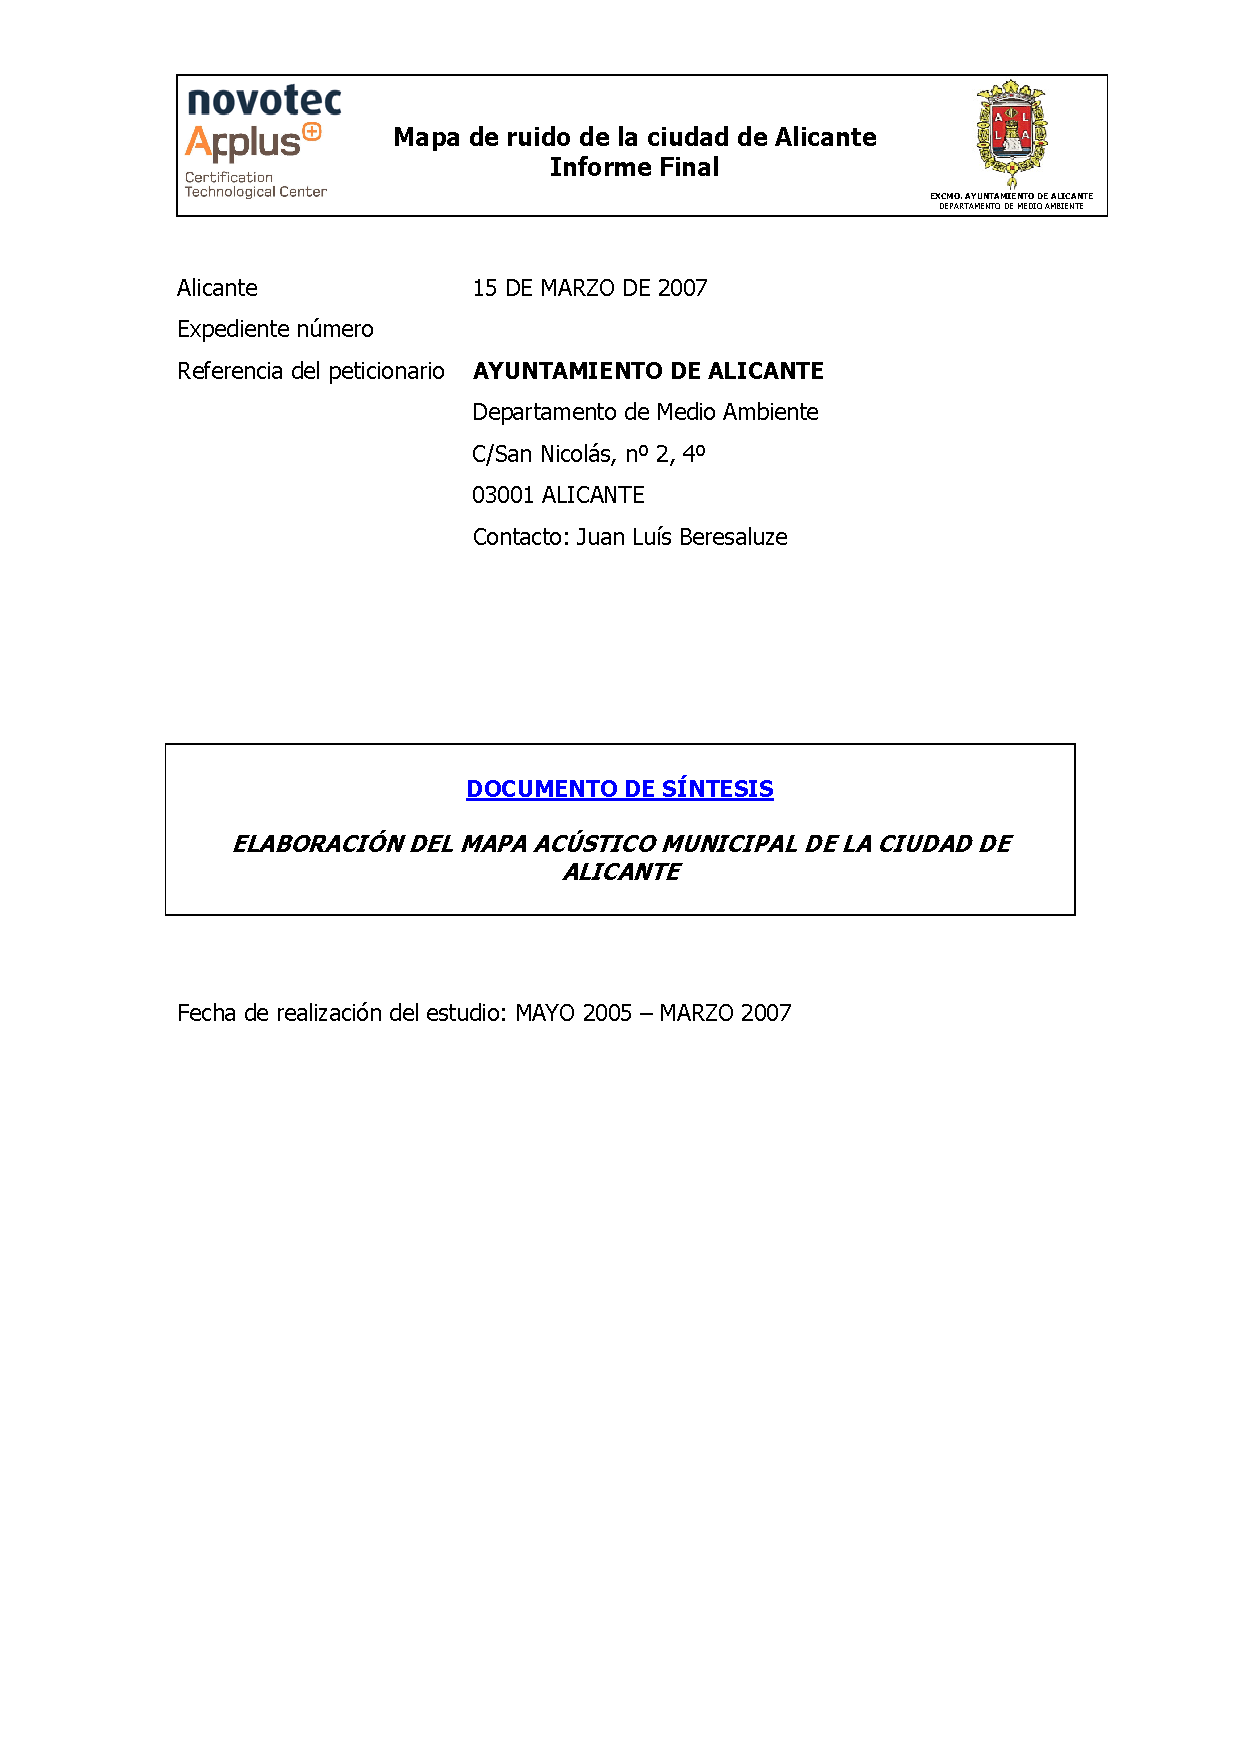
\includepdf[pages={1}]{archivos/ES_a_DF7_Agg_Alicante.pdf}

% Para incluir una página:
% [pages={0}] % Donde '0' es el número de la pagina del PDF que se quiere incluir

% Para incluir varias páginas consecutivas
% [pages={1-4}] % Con estos valores importa de la página 1 a la 4.

% Para incluir varias páginas salteadas
% [pages={1,4,7,10}] % Incluye las páginas 1,4,7 y 10

% Para incluir todo el documento PDF
% [pages=-]

% Si ademas de pages=... se incluye landscape, se importa en horizontal
% [pages{1},landscape]

\end{document}
